% MBS Master's Degree Dissertation - TU Faculty of Management
% Topic: VALUE RELEVANCE OF ACCOUNTING INFORMATION BEFORE AND AFTER THE BANKING CONSOLIDATION WAVE: EVIDENCE FROM NEPALESE COMMERCIAL BANKS
% Candidate: Asmita Subedi | Triveni International College
% Format source: Master's Degree Dissertation Guidelines 2019, Office of the Dean, FOM, TU
% Engine: xelatex + bibtex
%
% ARCHITECTURE (2026-10-29, config phase): this file is assembly ONLY.
% All packages, formatting, notation macros, and float layouts live in
% config/ (see config/preamble.tex). To change how the thesis looks,
% edit config/. To change what it says, edit chapters/, front/, or
% appendices/. This file must never again contain a \usepackage, a
% margin/font/spacing value, a heading format, or a page-style definition.
\documentclass[12pt,a4paper,oneside]{report}

% ============================================================================
% TU FOM MBS dissertation — configuration: packages and format.
%
% This file is the preamble that used to live inside main.tex. It was moved
% here verbatim on 2026-10-29 (config phase). No value was changed in the
% move, except for the one addition marked NEW below.
%
% RULE: this file holds packages and formatting only. It holds no chapter
% text, no table data, and no front-matter wording. To change how the
% thesis looks, edit this file (or macros.tex / floats.tex). To change
% what the thesis says, edit a file under chapters/, front/, or
% appendices/ — never this file.
%
% Load order matters and is preserved exactly: fontspec/geometry first,
% content packages in the middle, apacite settings after apacite, and
% hyperref last. Do not reorder without checking the compile log.
% ============================================================================

\usepackage{fontspec}
\setmainfont{Times New Roman}

% Strict TU FOM Dissertation Guidelines 2019 (Page 21):
% Top: 2.54 cm, Bottom: 2.54 cm, Right: 2.54 cm, Left: 3.18 cm (for binding).
\usepackage[top=2.54cm,bottom=2.54cm,right=2.54cm,left=3.18cm]{geometry}

\usepackage{setspace}
\setstretch{1.5}                % true 1.5 line spacing for text per FOM 2019
\setlength{\parindent}{0pt}    % paragraphs start flush left
\setlength{\parskip}{10pt}     % standard paragraph separation
\usepackage{enumitem}           % single pitch lists without extra item gap
\setlist{itemsep=0pt,topsep=0pt,parsep=0pt}
% Main-content loop Round 2: extra line-breaking stretch so long
% unbreakable words do not stick into the margin. No wording changed.
\setlength{\emergencystretch}{2em}

\usepackage{titlesec}
\usepackage{titletoc}
\usepackage{fancyhdr}
\usepackage{graphicx}
\usepackage{booktabs}
\usepackage{array}
\usepackage{longtable}
% NEW (2026-10-29, config phase): loaded for the thesistable environment
% in floats.tex. Not yet used by any chapter, so it changes no output.
\usepackage{threeparttable}
\usepackage{etoolbox}
\AtBeginEnvironment{tabular}{\singlespacing}
\AtBeginEnvironment{longtable}{\singlespacing}
% FOM 2019 p. 20 lists quotations among the single-spaced elements.
\AtBeginEnvironment{quote}{\singlespacing}
\usepackage{needspace}
\usepackage{amsmath}
\usepackage{unicode-math}
\setmathfont{TeX Gyre Termes Math}
\usepackage{tikz}
\usetikzlibrary{shapes,arrows,positioning}

% APA sixth edition referencing (FOM Guidelines 2019 p. 13 & Appendix C)
\usepackage[natbibapa]{apacite}
\bibliographystyle{apacite}
\setlength{\bibhang}{36pt}
\setlength{\bibsep}{6pt}

\usepackage{caption}
\captionsetup{font={normalsize,bf},justification=justified,singlelinecheck=false}
\usepackage{hyperref}
\hypersetup{colorlinks=true,linkcolor=black,citecolor=black,urlcolor=black}

% TU-strict preliminary headings (FOM Guidelines 2019 p. 9)
\renewcommand{\contentsname}{Table of Contents}
\renewcommand{\listtablename}{List of Tables}
\renewcommand{\listfigurename}{List of Figures}

% Format Chapter headings matching TU FOM convention:
% "CHAPTER I", newline, "INTRODUCTION" (14pt bold centered)
\titleformat{\chapter}[display]
  {\normalfont\large\bfseries\centering\setstretch{1}}
  {\MakeUppercase{\chaptertitlename\ \thechapter}}
  {6pt}
  {\MakeUppercase}
% Chapter numbers display in Roman (the thesis prose convention:
% Chapter I..V), while section, table, figure, and equation numbers
% stay Arabic. \thechapter itself is Roman, so the dependent
% counters are pinned to \arabic{chapter} explicitly; a bare
% \thechapter change alone would renumber them to IV.1, Table IV.1.
\renewcommand{\thechapter}{\Roman{chapter}}
\renewcommand{\thesection}{\arabic{chapter}.\arabic{section}}
\renewcommand{\thetable}{\arabic{chapter}.\arabic{table}}
\renewcommand{\thefigure}{\arabic{chapter}.\arabic{figure}}
\renewcommand{\theequation}{\arabic{chapter}.\arabic{equation}}
\titlespacing*{\chapter}{0pt}{10pt}{20pt}

% Section and subsection headings (12pt bold)
\titleformat{\section}
  {\normalfont\normalsize\bfseries\setstretch{1}}
  {\thesection}{0.5em}{}
\titlespacing*{\section}{0pt}{14pt}{4pt}

% Main-content loop Round 2: \sloppy in the subsection before-code so a
% long subsection title wraps instead of sticking into the margin
% (4.3.2 title overflowed 16.17 pt before this; no page-count change).
\titleformat{\subsection}
  {\normalfont\normalsize\bfseries\setstretch{1}}
  {\thesubsection}{0.5em}{\sloppy}
\titlespacing*{\subsection}{0pt}{10pt}{2pt}

\titleformat{\subsubsection}
  {\normalfont\normalsize\bfseries\setstretch{1}}
  {\thesubsubsection}{0.5em}{}
\titlespacing*{\subsubsection}{0pt}{8pt}{2pt}

% TOC formatting (12pt Times New Roman, single spaced per FOM p. 20)
\titlecontents{chapter}
  [0em]
  {\addvspace{8pt}\normalfont\normalsize\bfseries}
  {\MakeUppercase{\chaptername\ \thecontentslabel:\ }}
  {}
  {\enspace\titlerule*[0.5pc]{.}\contentspage}

\titlecontents{section}
  [2.0em]
  {\addvspace{3pt}\normalfont\normalsize}
  {\contentslabel[\thecontentslabel]{2.0em}}
  {\hspace*{-2.0em}}
  {\enspace\titlerule*[0.5pc]{.}\contentspage}

\titlecontents{subsection}
  [4.2em]
  {\addvspace{1pt}\normalfont\normalsize}
  {\contentslabel[\thecontentslabel]{2.6em}}
  {\hspace*{-2.6em}}
  {\enspace\titlerule*[0.5pc]{.}\contentspage}

\setcounter{secnumdepth}{3}
\setcounter{tocdepth}{2}

% Page numbering per FOM 2019 p. 21:
% Front matter: lower case Roman numerals bottom centre (ii, iii, iv...).
% Main body: Arabic numerals (1, 2, 3...) at top right corner.
\fancypagestyle{frontmatter}{
  \fancyhf{}
  \fancyfoot[C]{\thepage}
  \renewcommand{\headrulewidth}{0pt}
}

% Plain style during front matter: Roman numerals bottom center (FOM 2019 p. 21)
\fancypagestyle{plain}{
  \fancyhf{}
  \fancyfoot[C]{\thepage}
  \renewcommand{\headrulewidth}{0pt}
}

\fancypagestyle{mainbody}{
  \fancyhf{}
  \fancyhead[R]{\thepage}
  \renewcommand{\headrulewidth}{0pt}
  \setlength{\headheight}{15pt}
}

% ============================================================================
% Shared assembly commands (NEW, 2026-10-29, config phase).
% These replace three blocks that used to be written out inline in main.tex.
% Each command does exactly what its old inline block did, at the same
% point in main.tex, so the output does not change.
% ============================================================================

% One front-matter list (Contents / Tables / Figures), single-spaced,
% on its own page, as in the old main.tex.
% Front-matter list pages (TOC, LOT, LOF): single-spaced, and each
% registers itself in the TOC, like the reference thesis does for its
% preliminary pages. #1 is the TOC entry text, #2 the list command.
% The entry is written after the \clearpage so it records this page.
\newcommand{\thesisFrontList}[2]{%
  \clearpage
  \addcontentsline{toc}{chapter}{#1}
  \begingroup
  \singlespacing
  \setlength{\parskip}{0pt}
  #2
  \endgroup
}

% Main-body chapter-start page style: Arabic numerals top right
% (FOM p. 21). Old main.tex redefined plain at this point; this command
% is called at exactly that point instead.
\newcommand{\thesisMainbodyPlain}{%
  \fancypagestyle{plain}{
    \fancyhf{}
    \fancyhead[R]{\thepage}
    \renewcommand{\headrulewidth}{0pt}
    \setlength{\headheight}{15pt}
  }%
}

% Appendix chapter headings. Old main.tex redefined \titleformat just
% before the appendices; this command is called at exactly that point.
\newcommand{\thesisAppendixHeadings}{%
  % TOC entries for appendices must read APPENDIX, not CHAPTER: the
  % TOC is typeset before \appendix runs, when \chaptername is still
  % "Chapter". This line lands in the .toc file ahead of the appendix
  % entries, so from the next pass on they render as APPENDIX A/B/C.
  \addtocontents{toc}{\protect\renewcommand{\protect\chaptername}{Appendix}}%
  \titleformat{\chapter}[display]
    {\normalfont\large\bfseries\centering\setstretch{1}}
    {\MakeUppercase{Appendix\ \thechapter}}
    {6pt}
    {\MakeUppercase}%
  % \appendix has already set \thechapter to \Alph, so restoring the
  % chapter-based counter forms gives Appendix tables/figures A.1,
  % not 6.1 (the \arabic{chapter} forms above would give 6.1 here).
  \renewcommand{\thesection}{\thechapter.\arabic{section}}%
  \renewcommand{\thetable}{\thechapter.\arabic{table}}%
  \renewcommand{\thefigure}{\thechapter.\arabic{figure}}%
  \renewcommand{\theequation}{\thechapter.\arabic{equation}}%
}

% References (APA 6th edition, single spaced with hanging indent
% per FOM p. 20). Old main.tex wrote this block out inline.
\newcommand{\thesisBibliography}{%
  \phantomsection
  \addcontentsline{toc}{chapter}{References}
  \begingroup
  \singlespacing
  \urlstyle{APACsame}
  \bibliography{references}
  \endgroup
}

% ============================================================================
% TU FOM MBS dissertation — notation macros.
%
% STATUS (2026-10-29, config phase): DEFINED, NOT YET USED IN CHAPTERS.
% Chapters still use the inline forms. That is deliberate: defining a
% macro changes nothing, while converting chapters is a separate phase
% with its own replacement checklist and diff gate. Do not mix the two.
%
% RULE: name a command for what a symbol means, not how it looks.
% Each definition below expands to exactly the inline form currently
% used in the chapters, so the first converted version of a chapter
% must render identically. A notation restyle is a separate, approved
% decision after conversion, never bundled into it.
% ============================================================================

% Market price per share at the reporting deadline.
\newcommand{\MPSRD}{\ensuremath{\mathit{MPS}^{RD}}}
% Consolidation period indicator (Post = 1 for FY 2079/80-2081/82).
\newcommand{\Post}{\ensuremath{\mathit{Post}_t}}
% Two-way fixed effects.
\newcommand{\bankFE}{\ensuremath{\mu_i}}
\newcommand{\yearFE}{\ensuremath{\lambda_t}}
% Pre-consolidation slopes (Model 1, and Model 2 baseline).
\newcommand{\betaE}{\ensuremath{\beta_E}}
\newcommand{\betaB}{\ensuremath{\beta_B}}
% Regime-shift (interaction) coefficients (Model 2).
\newcommand{\deltaE}{\ensuremath{\delta_E}}
\newcommand{\deltaB}{\ensuremath{\delta_B}}
% Variable names, upright in maths contexts.
\newcommand{\EPS}{\ensuremath{\mathrm{EPS}}}
\newcommand{\BVPS}{\ensuremath{\mathrm{BVPS}}}
\newcommand{\ROA}{\ensuremath{\mathrm{ROA}}}
\newcommand{\DPS}{\ensuremath{\mathrm{DPS}}}
% Units and labels.
\newcommand{\NPR}{NPR}
\newcommand{\FY}[1]{FY #1}

% ============================================================================
% TU FOM MBS dissertation — table and figure environments.
%
% STATUS (2026-10-29, config phase): DEFINED, NOT YET USED IN CHAPTERS.
% Chapters still build tables and figures inline. That is deliberate:
% converting floats is a separate phase with its own LOT/LOF gate.
% Do not convert a table or figure here and in a chapter at the same
% time; one phase, one gate.
%
% RULE: a chapter supplies caption, label, header row, and data rows.
% Everything else — centring, size, caption style, booktabs rules,
% and note layout — comes from here, so a layout change is one edit
% in this file, not fourteen edits across chapters.
% ============================================================================

% One standard thesis table: float + centring + \small + booktabs +
% a note that stays attached to the table (threeparttable).
% Usage:
%   \begin{thesistable}
%     \caption{...}\label{...}
%     \begin{tabular}{...} ... \end{tabular}
%     \tablenote{...}
%   \end{thesistable}
\newenvironment{thesistable}[1][!htbp]{%
  \begin{table}[#1]\centering\small\begin{threeparttable}%
}{%
  \end{threeparttable}\end{table}%
}

% Table note, in the style currently used in chapters: footnotesize,
% italic "Note." lead-in, attached to the table width.
\newcommand{\tablenote}[1]{%
  \begin{tablenotes}\footnotesize\item[]\textit{Note.} #1\end{tablenotes}%
}

% One standard thesis figure. Default width 0.88\textwidth is the
% current converter default and the most common width in the thesis.
% Pass a different width only where a figure genuinely needs it, and
% say why in a comment at the call site.
% Usage: \thesisfigure[0.72\textwidth]{figures/F2_correlation_heatmap.pdf}{Caption}{fig:label}
\newcommand{\thesisfigure}[4][0.88\textwidth]{%
  \begin{figure}[!htbp]\centering\includegraphics[width=#1]{#2}\caption{#3}\label{#4}\end{figure}%
}

% ============================================================================
% TU FOM MBS dissertation — metadata: single source of truth.
%
% RULE: values that appear in more than one place (title page, and any
% prose that names the candidate or campus) are defined here and read
% from here. Change a value here, and every page that uses it changes
% together. This file holds values only — no formatting, no packages.
%
% VALUES ARE UNCHANGED (2026-10-29, config phase). They are copied
% character-for-character from front/titlepage.tex as it stood before
% this file existed. In particular, the submitting name below is the
% title-page value as written; correcting it, if it ever needs
% correcting, is a one-line change here, subject to normal approval.
% ============================================================================

\newcommand{\thesistitle}{VALUE RELEVANCE OF ACCOUNTING INFORMATION BEFORE AND AFTER THE BANKING CONSOLIDATION WAVE: EVIDENCE FROM NEPALESE COMMERCIAL BANKS}
\newcommand{\thesisauthor}{Asmita Subedi}
\newcommand{\thesisroll}{67514/24}
\newcommand{\thesisregistration}{7-2-48-1060-2018}
\newcommand{\thesiscampus}{Triveni International College}
\newcommand{\thesisdate}{October, 2026}
\newcommand{\thesisdegree}{Master's Degree}
\newcommand{\thesisfaculty}{Faculty of Management}


\begin{document}

% =============================================================================
% PREFATORY SECTION (FOM Guidelines Appendix B)
% =============================================================================

% Title page: counted as page i, unnumbered. Roman numbering starts
% here (not after) so the Title Page TOC entry records page i.
\pagenumbering{roman}
\begin{titlepage}
\addcontentsline{toc}{chapter}{Title Page}
\thispagestyle{empty}
\singlespacing
\setlength{\parskip}{0pt}
\begin{center}

\vspace*{0.5cm}

{\fontsize{16}{20}\selectfont\bfseries \thesistitle\par}

\vspace{2.5cm}

{\fontsize{13}{16}\selectfont A Dissertation submitted to the Office of the Dean, Faculty of Management in partial fulfilment of the requirements for the Master's Degree\par}

\vspace{2.5cm}

{\fontsize{13}{16}\selectfont by\par}

\vspace{0.8cm}

{\fontsize{13}{16}\selectfont\bfseries \thesisauthor\par}
\vspace{0.3cm}
{\fontsize{12}{15}\selectfont Roll No: \thesisroll\par}
{\fontsize{12}{15}\selectfont Registration No: \thesisregistration\par}
{\fontsize{12}{15}\selectfont Campus: \thesiscampus\par}

\vfill

{\fontsize{12}{15}\selectfont Pokhara, Nepal\par}
{\fontsize{12}{15}\selectfont \thesisdate\par}

\end{center}
\end{titlepage}



% Front matter pagination continues at ii (bottom center)
\pagestyle{frontmatter}
\setcounter{page}{2}

% Certification of Authorship
\clearpage
\addcontentsline{toc}{chapter}{Certification of Authorship}
\thispagestyle{plain}
\frontPageTitle{Certification of Authorship}

\vspace{1.5cm}

\setstretch{1.5}
I hereby corroborate that I have researched and submitted the final draft of dissertation entitled \textbf{``VALUE RELEVANCE OF ACCOUNTING INFORMATION BEFORE AND AFTER THE BANKING CONSOLIDATION WAVE: EVIDENCE FROM NEPALESE COMMERCIAL BANKS''}. The work of this dissertation has not been submitted previously for the purpose of conferral of any degrees nor it has been proposed and presented as part of requirements for any other academic purposes.

The assistance and cooperation that I have received during this research work has been acknowledged. In addition, I declare that all information sources and literature used are cited in the reference section of the dissertation.

\vspace{3.5cm}

\begin{flushleft}
\fomSignatureFont
\textbf{Asmita Subedi}\\
Signature:\\
Date of submission:
\end{flushleft}



% Report of Research Committee
\clearpage
\addcontentsline{toc}{chapter}{Report of Research Committee}
\thispagestyle{plain}
\begin{center}
{\fontsize{14}{18}\selectfont\bfseries Report of Research Committee\par}
\end{center}

\vspace{1.5cm}

% NOTE (visual-reference pass): this page follows FOM 2019 Appendix B
% p. 25 exactly, as a filled-in form. The sentence keeps a dotted blank
% for the supervisor's name (unknown, never invented); the two
% supervisor blocks and the bordered date boxes are the template's own
% layout, including the second block's Name/Signature/Position order.
\setstretch{1.5}
Ms.~Asmita Subedi has defended research proposal entitled \textbf{``VALUE RELEVANCE OF ACCOUNTING INFORMATION BEFORE AND AFTER THE BANKING CONSOLIDATION WAVE: EVIDENCE FROM NEPALESE COMMERCIAL BANKS''} successfully. The research committee has registered the dissertation for further progress. It is recommended to carry out the work as per suggestions and guidance of supervisor \makebox[5cm]{\dotfill} and submit the thesis for evaluation and viva voce examination.

\vspace{2.5cm}

\singlespacing
\noindent
% Column math (text width 433 pt): left 0.46 = 199 pt holds the longest
% left label (head, 180 pt); box parbox 0.46 = 199 pt holds the longest
% box label (defended date, 193 pt) on one line. \null\dotfill (not
% bare \dotfill) is required inside the boxes: a bare \dotfill at the
% start of a line after \\ is discarded and renders nothing. The
% blocks are side-by-side [t] parboxes (not a tabular): a tabular
% p-column put each box level with its block's LAST line instead of
% its first, while [t] parboxes align the box label with the block's
% first line, as in the template.
{\setlength{\fboxsep}{8pt}
\parbox[t]{0.46\textwidth}{Name of Supervisor \dotfill\\Position: \dotfill\\Signature: \dotfill}\hspace{0.02\textwidth}\parbox[t]{0.52\textwidth}{\fbox{\parbox[t]{0.46\textwidth}{\textbf{Dissertation Proposal Defended Date:}\\[0.4cm]\null\dotfill}}}
\par\vspace{2.0cm}
\noindent\parbox[t]{0.46\textwidth}{Name of Supervisor \dotfill\\Signature: \dotfill\\Position: \dotfill}\hspace{0.02\textwidth}\parbox[t]{0.52\textwidth}{\fbox{\parbox[t]{0.46\textwidth}{\textbf{Dissertation Submitted Date:}\\[0.4cm]\null\dotfill}}}
\par\vspace{2.0cm}
\noindent\parbox[t]{0.46\textwidth}{Name of head of Research committee \dotfill\\Signature: \dotfill}\hspace{0.02\textwidth}\parbox[t]{0.52\textwidth}{\fbox{\parbox[t]{0.46\textwidth}{\textbf{Dissertation Viva Voce Date:}\\[0.4cm]\null\dotfill}}}}


% Approval Sheet
\clearpage
\thispagestyle{plain}
\begin{center}
{\fontsize{14}{18}\selectfont\bfseries Approval Sheet\par}
\end{center}

\vspace{1.5cm}

\setstretch{1.5}
We have examined the dissertation entitled \textbf{``VALUE RELEVANCE OF ACCOUNTING INFORMATION BEFORE AND AFTER THE BANKING CONSOLIDATION WAVE: EVIDENCE FROM NEPALESE COMMERCIAL BANKS''} presented by \textbf{Asmita Subedi} for the degree of \textbf{Master of Business Studies (MBS)}. We hereby certify that the dissertation is acceptable for the award of degree.

\vspace{2.5cm}

\singlespacing
\noindent
\begin{tabular}{@{}p{0.48\textwidth}@{\hspace{0.04\textwidth}}p{0.48\textwidth}@{}}
\underline{\hspace{6.5cm}} & \underline{\hspace{6.5cm}} \\
\textbf{Dissertation Supervisor} & \textbf{Internal Examiner} \\
Signature & Signature \\[2.0cm]

\underline{\hspace{6.5cm}} & \underline{\hspace{6.5cm}} \\
\textbf{External Examiner} & \textbf{Chairperson, Research Committee} \\
Signature & Signature \\
\end{tabular}

\vspace{2.0cm}

\noindent
\textbf{Date:} \underline{\hspace{5cm}}



% Acknowledgements
\clearpage
\thispagestyle{plain}
\begin{center}
{\fontsize{14}{18}\selectfont\bfseries Acknowledgements\par}
\end{center}

\vspace{1.0cm}

\setstretch{1.5}
This master's dissertation represents the culmination of rigorous academic inquiry conducted in partial fulfillment of the requirements for the degree of Master of Business Studies (MBS) under the Faculty of Management, Tribhuvan University. The completion of this study has been made possible through the invaluable guidance, constructive critique, and generous encouragement of numerous individuals and institutions.

First and foremost, I express my deepest intellectual gratitude and profound appreciation to my respected dissertation supervisor, whose scholarly insight, methodological rigor, and continuous guidance shaped the trajectory of this research. The constructive feedback provided throughout the stages of econometric formulation, data verification, and empirical interpretation has been instrumental in ensuring academic precision and adherence to standard research methodologies.

I extend my sincere thanks to the Head of the Research Committee and esteemed faculty members of Triveni International College for their administrative facilitation, intellectual support, and critical evaluation during the proposal defense and research colloquia. Their valuable feedback during the formative phases of this work enriched the analytical framework.

I am profoundly indebted to the regulatory authorities—Nepal Rastra Bank (NRB) and the Securities Board of Nepal (SEBON)—as well as the Nepal Stock Exchange (NEPSE) for maintaining publicly accessible regulatory reports, macroeconomic bulletins, and historical trading archives. Special acknowledgement is due to the executive managements and investor relations departments of the sampled commercial banks—Global IME Bank Limited, Himalayan Bank Limited, Kumari Bank Limited, Nepal Investment Mega Bank Limited, and NMB Bank Limited—for making their comprehensive audited annual financial statements and corporate disclosures publicly available. I also express gratitude to financial information aggregators (ShareSansar, Merolagani, and FinancialNotices) for archiving historical secondary market trading data.

Finally, I convey my heartfelt gratitude to my family and friends for their enduring patience, moral encouragement, and unconditional support throughout the demanding period of my graduate studies. Their faith in my academic pursuits has been my constant source of strength.

\vspace{1.5cm}

\begin{flushright}
\singlespacing
\textbf{Asmita Subedi}\\
Triveni International College\\
Tribhuvan University
\end{flushright}



% Table of Contents (single-spaced per FOM p. 20)
\thesisFrontList{Table of Contents}{\tableofcontents}

% List of Tables
\thesisFrontList{List of Tables}{\listoftables}

% List of Figures
\thesisFrontList{List of Figures}{\listoffigures}

% List of Abbreviations
\clearpage
\thispagestyle{plain}
\begin{center}
{\fontsize{14}{18}\selectfont\bfseries List of Abbreviations\par}
\end{center}

\vspace{0.8cm}

\begingroup
\singlespacing
\setlength{\parskip}{0pt}
\begin{longtable}{@{}p{0.25\textwidth}p{0.70\textwidth}@{}}
\textbf{Abbreviation} & \textbf{Full Description} \\
\midrule
\endfirsthead
\textbf{Abbreviation} & \textbf{Full Description} \\
\midrule
\endhead
AGM & Annual General Meeting \\
AQR & Asset Quality Review \\
ASB & Accounting Standards Board (Nepal) \\
BAFIA & Banks and Financial Institutions Act \\
BFI & Banking and Financial Institution \\
BS & Bikram Sambat \\
BVPS & Book Value per Share \\
CBS & Core Banking Software \\
CCyB & Counter-Cyclical Capital Buffer \\
df & Degrees of Freedom \\
DPS & Dividend per Share \\
EPS & Earnings per Share \\
ESG & Environmental, Social, and Governance \\
FE & Fixed Effects \\
FOM & Faculty of Management \\
FY & Fiscal Year \\
GBIME & Global IME Bank Limited \\
HBL & Himalayan Bank Limited \\
HC3 & Heteroskedasticity-Consistent Covariance Estimator (MacKinnon \& White) \\
ICAN & Institute of Chartered Accountants of Nepal \\
KBL & Kumari Bank Limited \\
LM & Lagrange Multiplier \\
LTP & Last Traded Price \\
MBS & Master of Business Studies \\
MIS & Management Information Systems \\
MPS & Market Price per Share \\
$MPS^{RD}$ & Market Price per Share at Statutory Reporting Deadline \\
NAV & Net Asset Value \\
NEPSE & Nepal Stock Exchange Limited \\
NFRS & Nepal Financial Reporting Standards \\
NIB & Nepal Investment Bank Limited \\
NIMB & Nepal Investment Mega Bank Limited \\
NMB & NMB Bank Limited \\
NPL & Non-Performing Loan \\
NRB & Nepal Rastra Bank (Central Bank of Nepal) \\
OLS & Ordinary Least Squares \\
PAT & Profit After Tax \\
PEAD & Post-Earnings Announcement Drift \\
P/E & Price-to-Earnings Ratio \\
PPA & Purchase Price Allocation \\
RIV & Residual Income Valuation (Ohlson Framework) \\
ROA & Return on Assets \\
ROE & Return on Equity \\
SD & Standard Deviation \\
SE & Standard Error \\
SEBON & Securities Board of Nepal \\
SGM & Special General Meeting \\
TOC & Table of Contents \\
TU & Tribhuvan University \\
VIF & Variance Inflation Factor \\
\bottomrule
\end{longtable}
\endgroup



% Abstract
\clearpage
\thispagestyle{plain}
\begin{center}
{\fontsize{14}{18}\selectfont\bfseries Abstract\par}
\end{center}

\vspace{0.1cm}

\setstretch{1.5}
\setlength{\parskip}{3pt}
This dissertation investigates the value relevance of financial accounting information—specifically earnings per share (EPS) and book value per share (BVPS)—among prominent Nepalese commercial banks, and evaluates whether these valuation relationships underwent a structural regime shift following the commercial banking consolidation wave of early 2023. Grounded in the residual income valuation (RIV) framework of Ohlson (1995) and clean-surplus accounting theory, the study resolves critical methodological limitations in prior Nepalese literature by eliminating circular price-to-earnings (P/E) regressors, removing look-ahead bias via post-reporting-deadline prices under Section 59(2) of BAFIA ($MPS^{RD}$), and correcting for small-cluster downward bias. A longitudinal panel of five commercial banking series is examined across six fiscal years (FY 2076/77–2081/82, $N = 28$ clean bank-years under a 5-day freshness rule). Econometric estimation employs two-way fixed effects panel regressions with MacKinnon-White HC3 robust standard errors evaluated on Student's $t$ residual degrees of freedom.

In the baseline specification (Model 1), both earnings ($\hat{\beta}_E = 2.095, p = 0.616$) and book value ($\hat{\beta}_B = 0.219, p = 0.908$) exhibit positive but statistically insignificant slopes ($R^2 = 0.948$), showing that common fiscal-year fixed effects absorb macro-temporal price movements. In the regime shift specification (Model 2), pre-consolidation pricing was driven primarily by earnings on point estimates ($\hat{\beta}_E = 5.577, p = 0.140$), but post-consolidation interactions compressed implied slopes to $2.453$ for EPS and $-1.658$ for BVPS. The baseline joint Wald test fails to reject structural stability at the 5\% level ($F(2, 14) = 2.954, p = 0.085$). However, purging the entity-timing asymmetry in Specification R6 ($N = 23$) yields a statistically significant joint test at 5\% ($F(2, 10) = 5.82, p = 0.021$). The evidence demonstrates that the empirical regime shift is sensitivity-dependent rather than conclusive in the baseline, with post-merger credit provisioning and capital dilution coinciding with compressed multiples rather than book-value substitution. The study provides targeted policy implications for regulatory asset quality reviews, trading halt limits, and centralized electronic corporate filings.

\vspace{0.2cm}

\noindent
\textbf{Keywords:} Value Relevance, Commercial Banks, Bank Consolidation, Ohlson Model, Two-Way Fixed Effects.



% =============================================================================
% MAIN BODY OF THE DISSERTATION (Chapters I - V)
% =============================================================================

\clearpage
\pagestyle{mainbody}
\pagenumbering{arabic}
\setcounter{page}{1}

% Override plain style for main body chapter start pages: Arabic numerals top right (FOM p. 21)
\thesisMainbodyPlain

% Chapter I: Introduction
\chapter{Introduction}
\label{ch:introduction}

\section{Background of the Study}
\label{sec:background}

A central question in financial economics and accounting valuation is whether the empirical relationship between published financial statement numbers and equity market prices remains stable across structural corporate reorganizations. At its theoretical core, the valuation of common equity connects secondary market share prices to investors' expectations regarding a firm's future economic earning power, cash-flow generation capability, and net asset backing, conditioned upon the public and private information available in the marketplace \citep{beaver1968,fama1970}. Among competing valuation architectures, the residual income valuation (RIV) framework pioneered by \citet{ohlson1995} and \citet{feltham1995} provides an analytically rigorous and mathematically closed foundation linking financial accounting numbers directly to equity share prices. Anchored in the clean-surplus relation---which dictates that the change in book value of equity equals contemporaneous net income minus net dividends---the Ohlson framework establishes that a firm's equity market value can be expressed as the sum of its currently recognized book value of equity and the discounted present value of expected future residual income (abnormal earnings). Under linear information dynamics, this theoretical formulation demonstrates that market prices can be represented as a linear function of contemporaneous earnings per share (EPS) and book value per share (BVPS). In this framework, BVPS serves as an accounting proxy for the cumulative historical net assets contributed by shareholders and retained from past earnings, whereas EPS captures current operational profitability and serves as the baseline indicator of the firm's forward-looking earning capacity \citep{collins1997}.

Empirical studies investigating the association between equity prices and published accounting fundamentals---collectively recognized as the accounting value-relevance literature---have provided extensive documentation across developed, emerging, and frontier equity markets \citep{almumani2014,malhotra2013,sharma2011}. In frontier and developing market environments, however, the informational capacity of equity markets is frequently challenged by structural friction, regulatory evolution, asymmetric information, illiquidity, and corporate restructuring. The Nepalese capital market presents a distinct and compelling setting for examining the empirical validity and temporal stability of accounting value relevance. The organized secondary securities market in Nepal originated with the establishment of the Securities Exchange Centre in 1976 (2033 BS), which operated under the Securities Exchange Act, 1983. In 1993, a major financial-sector reform initiative restructured the Centre into the Nepal Stock Exchange (NEPSE) Limited as the nation's sole organized stock exchange, concurrently establishing the Securities Board of Nepal (SEBON) as the apex statutory securities market regulator. Floor trading on NEPSE officially commenced on 13 January 1994 (29 Poush 2050 BS) \citep{nepse2017}. Since its inception, NEPSE has been heavily dominated by the banking and financial institutions (BFIs) sector, with Class 'A' commercial banks constituting a major component of aggregate market capitalization, total annual trading turnover, and public equity ownership \citep{pradhan2016,timalsina2026}.

Nepal's commercial banking sector has experienced profound structural, regulatory, and institutional transformations over the past two decades. Following the financial liberalization policies initiated in the late 1980s, the number of licensed commercial banks expanded rapidly, reaching an apex of 32 licensed commercial banks alongside dozens of development banks and finance companies by fiscal year 2011/12 according to Nepal Rastra Bank institutional records \citep{adhikari2023,nrb2011}. Recognizing that severe institutional proliferation was outstripping supervisory capacity, inducing cutthroat lending competition, and creating systemic vulnerability, Nepal Rastra Bank (NRB)---the central bank and banking regulator---embarked on an aggressive, multi-phase consolidation drive. In 2011 (2068 BS), NRB introduced the \textit{Bank and Financial Institutions Merger and Acquisition Bylaws}, providing the initial regulatory architecture for voluntary corporate combinations \citep{nrb2011}. Subsequently, in its Monetary Policy for FY 2015/16 (2072/73 BS), NRB executed a historic fourfold capital expansion mandate, requiring all Class 'A' commercial banks to increase their minimum paid-up equity capital from NPR 2.0 billion to NPR 8.0 billion within a two-year regulatory window \citep{nrb2015}. Although banks initially satisfied this capital mandate primarily through bonus share capitalization and rights offerings, the persistent pressure for systemic consolidation culminated in the major banking consolidation wave of 2022--2023 (2079 BS). Supported by regulatory incentives and moral suasion, prominent commercial banks executed large-scale horizontal amalgamations and statutory acquisitions. By mid-October 2023 (Asoj 2080 BS), successive corporate consolidations reduced the commercial bank population to exactly 20 licensed institutions \citep{nrb2023list}.

A central theoretical and empirical issue in financial accounting is whether the valuation relationship between accounting fundamentals and equity market prices remains stable across major corporate reorganizations and structural transitions. As demonstrated in international M\&A literature, large-scale corporate mergers fundamentally restructure the corporate reporting entity: they alter the financial scale of the institution, introduce substantial post-merger integration costs, require accounting harmonization across legacy loan and deposit portfolios, generate non-recurring organizational adjustments, and expand the aggregate share capital base \citep{kwon2020}. Under such restructuring, reported accounting earnings can experience temporary impairment in transitoriness, volatility, and noise, potentially leading equity investors to discount earnings and rely more heavily on balance-sheet equity (book value) as a valuation anchor \citep{collins1997}. In Nepal, four of the country's most prominent commercial banking series---Global IME Bank Limited (GBIME), Himalayan Bank Limited (HBL), Kumari Bank Limited (KBL), and Nepal Investment Mega Bank Limited (NIMB)---commenced joint operations following amalgamations between January and February 2023 (Poush--Falgun 2079 BS). Concurrently, established peer institution NMB Bank Limited (NMB) maintained operational continuity without participating in the early-2023 consolidation wave, thereby providing a contemporaneous benchmark series. Although NMB had previously acquired Kanchan Development Bank Limited in August 2020 (adding approximately NPR 0.56 billion beyond its 13\% bonus share distribution to its share capital in FY 2077/78), it did not undergo horizontal amalgamation during the 2022--2023 consolidation wave, remaining structurally stable throughout the focal restructuring divide.

Despite the profound economic and corporate restructuring induced by the 2023 consolidation wave, empirical research on Nepalese commercial banking valuation reviewed in Chapter II has predominantly focused on static, sample-average regressions spanning multi-year historical periods without explicitly evaluating whether the fundamental accounting-price relationships shifted across the consolidation divide \citep{bhattarai2014,chaudhari2025,chhetri2023,gurungdahal2025,joshi2023,pant2024,timalsina2026}. Furthermore, conventional literature has routinely suffered from methodological shortcomings, notably the circular inclusion of price-derived valuation ratios such as Price-to-Earnings (P/E) as explanatory regressors predicting market prices, and the reliance on fiscal-year-end (Ashadh-end) pricing dates that precede the public disclosure of audited financial accounts. This dissertation directly addresses these theoretical, institutional, and empirical gaps by evaluating the value relevance of accounting information (EPS and BVPS) before and after Nepal's 2023 banking consolidation wave across a longitudinal panel of five commercial bank series over a six-year period (FY 2076/77 to FY 2081/82), using a standardized post-reporting-deadline pricing window grounded in Section 59(2) of the Banks and Financial Institutions Act, 2017 \citep{bafia2017}.

Previewing the empirical findings, the baseline two-way fixed-effects model yields positive but statistically insignificant slopes for both accounting fundamentals: earnings per share ($\hat{\beta}_E = 2.095$, HC3 $t = 0.51$, $p = 0.616$, with $16$ residual degrees of freedom) and book value per share ($\hat{\beta}_B = 0.219$, HC3 $t = 0.12$, $p = 0.908$). In the interaction specification (Model~2, with $14$ residual degrees of freedom), the pre-consolidation earnings slope is economically substantial but not statistically significant ($\hat{\beta}_E = 5.577$, $p = 0.140$), while the pre-consolidation book value slope is negligible ($\hat{\beta}_B = 0.100$, $p = 0.940$). The estimated post-consolidation shift parameters---$\hat{\delta}_E = -3.124$ ($p = 0.448$) and $\hat{\delta}_B = -1.758$ ($p = 0.175$)---imply compressed post-consolidation slopes of $\hat{\beta}_E + \hat{\delta}_E = 2.453$ for earnings and $\hat{\beta}_B + \hat{\delta}_B = -1.658$ for book value, but neither individual shift attains significance. The joint Wald test of structural change indicates parameter shift across regimes at the 10\% level ($F(2, 14) = 2.954, p = 0.085$), with structural instability confirmed at the 5\% level when the FY 2078/79 entity-timing mismatch is excluded ($F(2, 10) = 5.818, p = 0.021$).

\section{Problem Statement}
\label{sec:problem_statement}

The valuation behavior of commercial bank equities in emerging capital markets is governed by a complex interplay between institutional regulation, financial disclosure credibility, corporate scale, and investor sentiment. In Nepal, empirical investigations examining the association between accounting indicators and equity share prices have documented extensive but divergent findings. Prior studies have evaluated diverse financial measures, including earnings per share, book value per share, dividend per share, return on assets, return on equity, and price-earnings ratios, yet their reported empirical conclusions diverge sharply regarding coefficient magnitudes, directional signs, and statistical significance.

For instance, regarding operating profitability, \citet{chhetri2023} examined 13 commercial banks over 2012--2022 using pooled ordinary least squares (OLS) and reported a statistically significant positive association between return on assets (ROA) and market share price (MPS). Conversely, \citet{chaudhari2025} investigated ten commercial banks over 2014/15--2023/24 and documented a statistically significant \textit{negative} relationship between ROA and share prices, while \citet{gyawali2022} found a positive but statistically insignificant ROA coefficient across ten banks observed between 2017 and 2021. For book value per share, \citet{joshi2023} reported a strong, positive, statistically significant association with market price among seven commercial banks over 2012/13--2021/22, whereas \citet{pant2024} documented an insignificant negative coefficient for BVPS across seven commercial banks observed through FY 2023/24. Similarly, while \citet{bhandari2026} identified EPS as the predominant determinant of equity valuation across listed commercial banks, \citet{chhetri2023} and \citet{giri2024} found bivariate or multivariate EPS coefficients to be statistically negligible or secondary to dividend and net worth measures.

These empirical discrepancies stem fundamentally from differences in sample composition, observation periods, econometric specifications, and variable measurement timing. However, beyond empirical divergence across static studies, the existing literature reveals four critical conceptual and methodological problems that motivate the present dissertation:

\begin{enumerate}[label=\textbf{\arabic*.}]
\item \textbf{The Absence of Consolidation Regime Shift Analysis:}
Published Nepalese studies reviewed in this dissertation predominantly employ pooled OLS or static panel regression designs that estimate unconditional, full-sample average coefficients across their entire observation spans \citep{bhattarai2014,chaudhari2025,gurungdahal2025,timalsina2026}. These static models implicitly assume parameter stationarity---that the valuation multiple attached to a rupee of earnings or book value remains identical throughout the sample period. However, between January and February 2023, four prominent commercial banking mergers in recent Nepalese history commenced joint operations: Global IME Bank absorbed Bank of Kathmandu (9 January 2023); Himalayan Bank acquired Civil Bank (24 February 2023); Kumari Bank absorbed NCC Bank (1 January 2023); and Nepal Investment Bank amalgamated with Mega Bank Nepal to form NIMB (11 January 2023) \citep{gbime2022agm,hbl2023report,kumari2022sgm,nimb2023report}. These amalgamations fundamentally transformed the capital scale, loan portfolios, branch networks, and risk profiles of the surviving entities. International research demonstrates that structural corporate combinations alter the financial reporting environment, temporarily increasing earnings volatility while shifting investor attention toward balance-sheet net worth \citep{kwon2020}. No empirical study identified in the literature reviewed in Chapter II has formally evaluated whether the valuation coefficients of EPS and BVPS shifted between the pre-consolidation (FY 2076/77--2078/79) and post-consolidation (FY 2079/80--2081/82) periods using an explicit regime-interaction econometric framework.

\item \textbf{Econometric Endogeneity from Price-Derived Explanatory Variables:}
A common practice across studies reviewed in Chapter II is the inclusion of the price-earnings (P/E) ratio alongside fundamental accounting variables in regression models where Market Price per Share (MPS) serves as the dependent variable \citep{bhattarai2014,chhetri2023,giri2024,gurungdahal2025,joshi2023,pant2024}. Because the P/E ratio is algebraically defined as $\text{P/E} = \text{MPS} / \text{EPS}$, specifying a model of the form $\text{MPS}_{it} = \beta_0 + \beta_1 \text{EPS}_{it} + \beta_2 \text{P/E}_{it} + \dots$ embeds the dependent variable directly within the numerator of one of its own explanatory regressors. This introduces mechanical endogeneity, circular causality, and spurious correlation that severely distort the estimated coefficients and invalidate standard hypothesis testing. A methodologically defensible accounting valuation study must strictly exclude price-derived multiples and focus exclusively on fundamental accounting variables that are determined independently of secondary market trading prices.

\item \textbf{Temporal Misalignment and Look-Ahead Bias in Price Measurement:}
A critical limitation in prior Nepalese valuation research concerns the timing of share price measurement. Across the empirical studies reviewed in Chapter II, published literature predominantly uses fiscal-year-end (Ashadh-end / mid-July) closing market prices or annual volume-weighted average prices to evaluate the relevance of financial statement numbers \citep{bhattarai2014,pradhan2016,silwal2019}. Under Nepalese corporate and regulatory realities, commercial bank fiscal years terminate at Ashadh-end (mid-July), but audited annual financial statements are not prepared, audited by statutory auditors, approved by NRB, and published for months thereafter. Pairing Ashadh-end market prices with audited accounting figures that were not publicly known on that date creates severe look-ahead bias, violating the temporal causality required for information content studies \citep{ball1968,beaver1968,bernard1989}. Conversely, attempting to reconstruct individual, ad hoc corporate disclosure dates for 30 bank-year observations is fraught with measurement noise, selective informal leakage, and archival opacity. To resolve this temporal conundrum, an objective, legally grounded measurement rule is required. Section 59(2) of the Banks and Financial Institutions Act, 2017 (BAFIA) legally mandates that Class 'A' commercial banks publish their audited annual balance sheets and profit and loss accounts within nine months into the subsequent fiscal year---a statutory deadline operationalized at the end of Chaitra (mid-April) of the subsequent fiscal year \citep{bafia2017}. Observing market prices at a standardized window immediately following this statutory threshold ensures that audited financial information was legally required to be public, avoiding both look-ahead bias and timestamp reconstruction ambiguity.

\item \textbf{Neglect of Degrees of Freedom and Small-Cluster Econometric Fragility:}
Prior single-sector panel studies in Nepal frequently implement econometric estimation without disclosing or addressing the severe statistical constraints imposed by small cross-sectional dimensions. In fixed-effects panel models with interactive specifications, parameter proliferation rapidly consumes residual degrees of freedom. On a clean sample of $N = 28$ observations, estimating individual bank fixed effects, common fiscal-year fixed effects, and four slope coefficients leaves exactly $28 - 14 = 14$ residual degrees of freedom. Furthermore, standard cluster-robust sandwich standard errors perform poorly and exhibit substantial finite-sample downward bias when the number of clusters is small ($G = 5$) \citep{cameron2008clusters}. Prior empirical studies in Nepal reviewed in Chapter II have largely left these inferential hazards unaddressed, risking false discoveries and overstated statistical precision. Rigorous modeling requires explicit parameter accounting and the deployment of MacKinnon-White HC3 heteroskedasticity-robust inference, accompanied by transparent non-causal interpretation.
\end{enumerate}

To address these empirical, methodological, and econometric problems, this study investigates three central research questions:
\begin{enumerate}[label=\textbf{\arabic*.}]
\item \textbf{Research Question 1:} Are fundamental accounting measures---specifically earnings per share (EPS) and book value per share (BVPS)---statistically associated with post-reporting-deadline market share prices ($MPS^{RD}$) among the selected Nepalese commercial banks?
\item \textbf{Research Question 2:} Did the estimated valuation associations of EPS and BVPS with market share prices differ significantly between the pre-consolidation period (FY 2076/77--2078/79) and the post-consolidation period (FY 2079/80--2081/82)?
\item \textbf{Research Question 3:} Are the baseline and consolidation-interaction findings robust to alternative operating profitability specifications, inclusion of eligible dividend disclosures, adjustment for bonus share capitalization, retrospective earnings restatements, and the econometric exclusion of structural transition periods?
\end{enumerate}

\section{Objectives of the Study}
\label{sec:objectives}

The overarching general objective of this dissertation is to examine the accounting value relevance of financial information and evaluate whether the empirical relationships between accounting fundamentals and equity market prices differed before and after the 2023 commercial banking consolidation wave across five purposively selected commercial bank series in Nepal.

To achieve this general objective, the study establishes the following specific objectives:
\begin{enumerate}[label=\textbf{\arabic*.}]
\item \textbf{To estimate the baseline value relevance} of earnings per share (EPS) and book value per share (BVPS) in relation to secondary market share prices measured at a standardized post-reporting-deadline window ($MPS^{RD}$) within a two-way fixed-effects panel regression framework.
\item \textbf{To test whether the empirical valuation slopes} of EPS ($\beta_E$) and BVPS ($\beta_B$) differed between the pre-consolidation period (FY 2076/77--2078/79) and the post-consolidation period (FY 2079/80--2081/82) by evaluating interaction parameters ($\delta_E, \delta_B$) and a joint Wald coefficient test.
\item \textbf{To evaluate the econometric robustness and stability} of the value-relevance estimates across alternative specifications, including:
\begin{itemize}
\item Substituting return on assets (ROA) for EPS as an asset-scaled profitability measure;
\item Incorporating eligible cash dividend per share (DPS) declarations into the valuation equation;
\item Sensitivity analysis excluding the FY 2079/80 merger transition year to verify results are not driven by immediate consolidation shock;
\item Sensitivity analysis excluding FY 2078/79 to address entity-timing mismatch between standalone fundamentals and consolidated trading prices;
\item Re-estimation using bonus-adjusted per-share metrics to account for share capital dilutions; and
\item Re-estimation using retrospective audited basic EPS restatements from subsequent annual reports.
\end{itemize}
\end{enumerate}

\section{Hypotheses of the Study}
\label{sec:hypotheses}

The research hypotheses formulated in this dissertation are directly anchored in the residual income valuation theory of \citet{ohlson1995}, the post-merger value-relevance framework of \citet{kwon2020}, and empirical findings from emerging capital markets. Under Ohlson's (1995) theoretical model, both contemporaneous earnings and book equity are expected to correlate positively with market prices because they reflect, respectively, current operating efficiency and accumulated net asset value. However, following the methodological conventions of empirical accounting, all hypotheses are tested two-tailed at the 5\% level of significance ($\alpha = 0.05$) without imposing directional signs, thereby allowing the empirical data to support or fail to support the theoretical predictions.

The hypotheses are grouped into two categories corresponding to the baseline value-relevance model (Model 1) and the consolidation-interaction model (Model 2):

\subsection{Category A: Baseline Value Relevance Hypotheses (Model 1)}
\begin{itemize}
\item \textbf{Hypothesis 1 ($H_1$):}
\begin{itemize}
\item Null hypothesis ($H_{0,1}$): Earnings per share (EPS) is not significantly associated with secondary market share price at the reporting-deadline window in the baseline two-way fixed-effects model.
\begin{equation}
H_{0,1}: \beta_E = 0
\end{equation}
\item Alternative hypothesis ($H_{a,1}$): Earnings per share (EPS) is significantly associated with secondary market share price at the reporting-deadline window in the baseline two-way fixed-effects model.
\begin{equation}
H_{a,1}: \beta_E \ne 0
\end{equation}
\end{itemize}

\item \textbf{Hypothesis 2 ($H_2$):}
\begin{itemize}
\item Null hypothesis ($H_{0,2}$): Book value per share (BVPS) is not significantly associated with secondary market share price at the reporting-deadline window in the baseline two-way fixed-effects model.
\begin{equation}
H_{0,2}: \beta_B = 0
\end{equation}
\item Alternative hypothesis ($H_{a,2}$): Book value per share (BVPS) is significantly associated with secondary market share price at the reporting-deadline window in the baseline two-way fixed-effects model.
\begin{equation}
H_{a,2}: \beta_B \ne 0
\end{equation}
\end{itemize}
\end{itemize}

\subsection{Category B: Consolidation-Period Regime Shift Hypotheses (Model 2)}
In corporate reorganizations, international research suggests that post-merger integration costs, portfolio revaluation, and organizational disruption may temporarily increase earnings noise, potentially leading investors to place relatively greater valuation weight on balance-sheet book value \citep{kwon2020}. However, whether this shift manifested in Nepal's emerging banking sector remains an open empirical question. Accordingly, the interaction hypotheses test for parameter differences across periods:
\begin{itemize}
\item \textbf{Hypothesis 3 ($H_3$):}
\begin{itemize}
\item Null hypothesis ($H_{0,3}$): The slope coefficient linking earnings per share to market share price does not differ significantly between the pre-consolidation and post-consolidation periods.
\begin{equation}
H_{0,3}: \delta_E = 0
\end{equation}
\item Alternative hypothesis ($H_{a,3}$): The slope coefficient linking earnings per share to market share price differs significantly between the pre-consolidation and post-consolidation periods.
\begin{equation}
H_{a,3}: \delta_E \ne 0
\end{equation}
\end{itemize}

\item \textbf{Hypothesis 4 ($H_4$):}
\begin{itemize}
\item Null hypothesis ($H_{0,4}$): The slope coefficient linking book value per share to market share price does not differ significantly between the pre-consolidation and post-consolidation periods.
\begin{equation}
H_{0,4}: \delta_B = 0
\end{equation}
\item Alternative hypothesis ($H_{a,4}$): The slope coefficient linking book value per share to market share price differs significantly between the pre-consolidation and post-consolidation periods.
\begin{equation}
H_{a,4}: \delta_B \ne 0
\end{equation}
\end{itemize}
\end{itemize}

The overarching econometric evaluation of structural change across the banking consolidation wave is conducted via the joint null and alternative hypotheses:
\begin{equation}
H_{0,\text{joint}}: \delta_E = 0 \text{ and } \delta_B = 0 \quad \text{versus} \quad H_{a,\text{joint}}: \delta_E \ne 0 \text{ or } \delta_B \ne 0
\end{equation}
Rejecting this joint null hypothesis provides statistical evidence that the overall accounting-price valuation relationship differed across the consolidation period. In accordance with rigorous observational econometrics, non-rejection or rejection of these parameters is interpreted strictly as observed differences in statistical associations across calendar regimes, rather than as causal impacts of bank mergers.

\section{Rationale and Significance of the Study}
\label{sec:rationale}

This dissertation is justified on theoretical, methodological, empirical, and practical grounds. As Nepal's commercial banking sector emerges from the structural consolidation wave of 2022--2023, understanding how capital markets perceive and price accounting disclosures is critical for financial transparency, capital allocation, and regulatory design. The specific rationale and significance of this research include:

\begin{enumerate}[label=\textbf{\arabic*.}]
\item \textbf{Theoretical and Conceptual Contribution:}
While the residual income valuation framework of \citet{ohlson1995} has been extensively tested in developed equity markets, its applicability in frontier environments undergoing rapid structural transformation remains underexplored. By synthesizing Ohlson's (1995) valuation model with the post-merger value-relevance framework of \citet{kwon2020}, this study provides a coherent theoretical structure for assessing how corporate amalgamations alter the relative informational roles of income-statement flows (earnings) versus balance-sheet stocks (book value). It grounds the empirical valuation of Nepalese banks within formal accounting valuation theory.

\item \textbf{Methodological Rigor and Standardization of Observation Timing:}
A major contribution of this study is the development and implementation of an institutionally grounded, reproducible price-measurement protocol ($MPS^{RD}$). By operationalizing the statutory nine-month reporting deadline under Section 59(2) of BAFIA at the end of Chaitra (mid-April), the study addresses the temporal flaw of prior Nepalese studies that paired Ashadh-end market prices with financial reports published up to nine months later. In observed corporate practice across the sampled banks, audited financial highlights and dividend declarations are typically published between Ashwin and Poush (October to January), with formal AGM proceedings concluded prior to the end-of-Chaitra reporting deadline operationalized in this study. Observing market prices at the first trading session following the Chaitra deadline ensures that audited financial accounts were legally required to be in the public domain under BAFIA Section 59(2) prior to price observation, while avoiding the measurement error and selective leakage inherent in attempting to reconstruct unverified corporate press-release timestamps across historical periods. Furthermore, the explicit formulation of a 5-day freshness rule---under which trading-suspended observations are treated as missing rather than imputed from stale dates---maintains empirical transparency and eliminates stale price contamination.

\item \textbf{Econometric Integrity through Exclusion of Mechanical Multiples:}
This dissertation explicitly corrects the pervasive econometric specification error in Nepalese literature: the inclusion of P/E ratios alongside EPS in models predicting share prices. By excluding price-derived multiples and demonstrating the severe collinearity between EPS and ROA ($r = 0.975$, yielding variance inflation factors between approximately 20 and 30 depending on model specification), this study avoids the mechanical simultaneity bias inherent in price-deflated multiple regressions. It demonstrates why ROA must be evaluated as an alternative substitute rather than an additive regressor, preventing spurious statistical inferences.

\item \textbf{Practical Significance for Capital Market Stakeholders:}
The findings of this study provide actionable insights for diverse capital market participants:
\begin{itemize}
\item \textbf{Individual and Institutional Investors:} Informs investors on NEPSE regarding the comparative valuation relevance of earnings versus book values across structural consolidation periods, highlighting the valuation noise associated with transitional merger accounting.
\item \textbf{Commercial Bank Management and Boards of Directors:} Informs bank executives regarding the capital-market consequences of earnings volatility, dividend payout stability, and balance-sheet transparency following corporate amalgamations.
\item \textbf{Nepal Rastra Bank (NRB):} Offers the central bank empirical observations on how secondary equity markets evaluate capital and earnings metrics surrounding policy-driven bank consolidations, assisting in the design of future prudential capital and reporting guidelines.
\item \textbf{Securities Board of Nepal (SEBON) and NEPSE:} Highlights the critical importance of timely corporate disclosures, centralized announcement timestamp databases, and the market-distorting effects of prolonged merger-related trading suspensions.
\item \textbf{Academic Researchers:} Provides a documented, reproducible dataset and analytical codebase, rigorous two-way fixed-effects methodology, and robust finite-sample econometric protocols for future researchers investigating financial-sector dynamics in South Asia.
\end{itemize}
\end{enumerate}

\section{Limitations of the Study}
\label{sec:limitations}

To maintain academic integrity and assist readers in interpreting the findings within their proper context, the methodological, institutional, and empirical boundaries of this research are explicitly acknowledged. In accordance with the \textit{Master's Degree Dissertation Guidelines (2019)} of the Faculty of Management, a clear distinction is maintained between the scope of the study (which defines its deliberate boundaries) and the limitations that arise within that scope:

\begin{enumerate}[label=\textbf{\arabic*.}]
\item \textbf{Small Purposive Sample and Sectoral Generalizability:}
The study's scope is confined to five purposively selected Class 'A' commercial bank series observed across six fiscal years (FY 2076/77 to FY 2081/82). While these five institutions represent the central corporate combinations of the 2023 consolidation wave alongside an unmerged benchmark (in the 2023 wave), the sample cannot be generalized to the entire commercial banking industry, development banks, finance companies, or non-financial listed sectors. Findings apply directly to the selected institutions and their specific consolidation contexts.

\item \textbf{Realized Sample Attrition Due to Trading Suspensions:}
Although primary audited annual financial statements were complete for all 30 target bank-year observations, prolonged merger-related trading suspensions rendered two pre-consolidation market price observations unverifiable within the 5-day freshness window: Himalayan Bank FY 2077/78 (merger-related trading suspension until 6 June 2022; 54 days late) and Nepal Investment Bank FY 2077/78 (merger-related trading suspension until 30 May 2022; 47 days late). Consequently, following strict research protocol, these two observations are coded as missing rather than imputed from stale pre-suspension prices, reducing the clean estimation sample to $N = 28$ observations (13 pre-consolidation, 15 post-consolidation).

\item \textbf{Econometric Fragility and Finite-Sample Constraints:}
Estimating two-way fixed effects (bank fixed effects $\mu_i$ and fiscal-year fixed effects $\lambda_t$) in conjunction with four slope parameters on a sample of $N = 28$ observations leaves exactly $28 - 14 = 14$ residual degrees of freedom in Model 2. Furthermore, standard cluster-robust standard errors fail to perform reliably when the number of clusters is very small ($G = 5$) \citep{cameron2008clusters}. Although the study mitigates heteroskedasticity by deploying MacKinnon-White HC3 robust standard errors, all statistical tests must be interpreted as exploratory indicators rather than definitive asymptotic proofs.

\item \textbf{Calendar-Period Operationalization vs. Causal Identification:}
The pre-consolidation (FY 2076/77--2078/79) and post-consolidation (FY 2079/80--2081/82) regimes are defined by calendar time. Consequently, the estimated interaction parameters ($\delta_E, \delta_B$) capture overall shifts in accounting-price associations across these temporal periods. These shifts reflect not only the internal corporate effects of banking consolidation, but also contemporaneous macroeconomic shifts, interest rate fluctuations, NEPSE broad-index cycles, and post-pandemic economic adjustments. The research design does not identify the isolated causal impact of mergers.

\item \textbf{Entity-Timing Mismatch in FY 2078/79:}
Because the four merging banks commenced joint operations in January--February 2023 (mid-FY 2079/80), their FY 2078/79 audited financial accounts represent pre-merger standalone operations, whereas their post-reporting-deadline market prices observed in mid-April 2023 reflect post-merger consolidated trading. Although this transition mismatch is retained in the baseline models to preserve sample continuity, it represents an unavoidable institutional friction that is explicitly evaluated via sensitivity exclusions.

\item \textbf{Institutional Reporting Compliance and Information Leakage:}
The standardized reporting window relies on the legal mandate under BAFIA Section 59(2) requiring publication within nine months into the subsequent fiscal year. While in the disclosures examined for this study, commercial bank boards typically released audited highlights and dividend proposals between Ashwin and Poush (months prior to the Chaitra statutory deadline), this pattern reflects observed corporate practice rather than audited proof of disclosure timing for every individual observation; any unrecorded informal information leakage prior to public board announcements remains an unobservable institutional feature of frontier equity markets.
\end{enumerate}

\section{Organization of the Study}
\label{sec:organization}

This dissertation is organized into five chapters, structured in accordance with the \textit{Master's Degree Dissertation Guidelines (2019)} of the Faculty of Management, Tribhuvan University:

\begin{itemize}
\item \textbf{Chapter I: Introduction:} Provides the contextual background of the study, presents the problem statement, outlines the research questions, defines the general and specific objectives, states the research hypotheses, justifies the rationale and significance of the study, acknowledges the research limitations, and outlines the overall chapter structure.
\item \textbf{Chapter II: Literature Review:} Reviews the theoretical underpinnings of equity valuation, including the Ohlson (1995) residual income valuation framework, post-merger value-relevance theory, signaling theory, agency theory, and efficient market dynamics. Systematically reviews international and Nepalese empirical studies on banking valuation, examines the evolution of merger regulations in Nepal, and synthesizes the identified literature gaps that this study addresses.
\item \textbf{Chapter III: Research Methodology:} Explains the quantitative, correlational, and comparative panel research design. Details the target population, purposive sampling criteria, and profile of the five sampled commercial bank series. Specifies the secondary data sources, operational variable definitions ($MPS^{RD}$, EPS, BVPS, ROA, DPS, $\mathit{Post}_t$), and variable measurement rules. Formulates the baseline and consolidation-interaction two-way fixed-effects models, details the MacKinnon-White HC3 econometric estimation procedure, outlines the diagnostic tests, and specifies the eight-specification estimation and robustness suite (R1--R2 baselines plus six robustness variants R3--R8).
\item \textbf{Chapter IV: Results and Discussion:} Presents the empirical findings derived from the analysis pipeline. Details descriptive statistics across full, pre-, and post-consolidation periods; presents the Pearson correlation matrix and screens for multicollinearity; reports parameter estimates and hypothesis test results for Model 1 (baseline) and Model 2 (interaction); presents the joint Wald $F$-test of structural shift; reports the results of the eight-specification estimation and robustness suite; presents econometric diagnostic tests (VIF, Breusch-Pagan, Cook's distance, normality); and provides a structured discussion contextualizing the empirical findings with prior Nepalese and international literature.
\item \textbf{Chapter V: Summary and Conclusion:} Summarizes the entire study, synthesizing the core empirical findings regarding earnings and book value relevance across the consolidation wave. Draws overarching conclusions based on the statistical evidence, outlines actionable policy and managerial implications for investors, bank executives, and regulatory authorities (NRB, SEBON), and offers recommendations for future academic research.
\end{itemize}

Following the main body of the dissertation, a complete \textbf{References} section compiled in APA 6th edition format provides full bibliographic details for all cited literature, statutes, and reports. A comprehensive \textbf{Appendices} section contains supplementary tables (price verification records, specification comparisons, full regression dataset) and appendix diagnostic figures.



% Chapter II: Literature Review
\chapter{Literature Review}
\label{ch:literature_review}

\section{Introduction}
\label{sec:lit_intro}

The purpose of this chapter is to conduct an extensive, critical, and structured review of the theoretical, regulatory, and empirical literature pertinent to the valuation of equity securities and the value relevance of financial accounting information, with specific focus on commercial banking institutions undergoing structural consolidation.

This chapter establishes a direct link with the research problem and objectives articulated in Chapter~I. It is organized into four major substantive sections:
\begin{itemize}
\item \textbf{Section~\ref{sec:theoretical_review}: Theoretical Review} examines the foundational economic and financial accounting theories that govern equity valuation, residual income dynamics, post-merger information environments, market efficiency, signaling, agency conflicts, and the econometric hazards of price-derived valuation multiples.
\item \textbf{Section~\ref{sec:regulatory_framework}: Review of Legal, Regulatory, and Policy Framework in Nepal} reviews the institutional architecture governing the Nepalese banking sector and capital market, including the regulatory mandates of Nepal Rastra Bank (NRB), the statutory reporting obligations under the Banks and Financial Institutions Act (BAFIA), 2017, and the policy evolution of bank merger directives and capital expansion mandates.
\item \textbf{Section~\ref{sec:empirical_review}: Empirical Review} provides a comprehensive, comparative analysis of prior empirical studies, divided into international investigations across developed and emerging capital markets, foundational Nepalese banking studies, recent investigations of share price determinants (2021--2024), and contemporary literature spanning the early-2023 consolidation wave (2024--2026), synthesized through a detailed summary matrix.
\item \textbf{Section~\ref{sec:research_gap}: Research Gap} synthesizes the critical methodological, econometric, and conceptual shortcomings of the existing literature and explicitly articulates how the present dissertation addresses each identified gap.
\end{itemize}

\section{Theoretical Review}
\label{sec:theoretical_review}

\subsection{The Residual Income Valuation (RIV) Framework}
\label{subsec:ohlson_framework}

In financial economics and accounting theory, equity valuation has evolved from dividend-discounting formulations into models grounded in fundamental accounting numbers. The seminal theoretical breakthrough linking financial accounting disclosures directly to equity market values was established by \citet{ohlson1995} and extended by \citet{feltham1995}. The Residual Income Valuation (RIV) framework---often designated as the Edwards-Bell-Ohlson (EBO) model---reconceptualizes firm value by expressing the market value of common equity as the sum of currently recognized book value of equity and the present value of expected future residual income (abnormal earnings).

The mathematical foundation of the Ohlson framework rests on four interrelated structural building blocks:

\begin{enumerate}[label=\textbf{\arabic*.}]
\item \textbf{The Present Value of Expected Dividends (PVED):}
Consistent with neoclassical asset pricing theory, the intrinsic market value of a firm's common equity at date $t$ ($P_t$) equals the discounted present value of all expected future net cash distributions (dividends, $D_{t+\tau}$) paid to equity holders:
\begin{equation}
P_t = \sum_{\tau=1}^{\infty} \frac{\mathbb{E}_t[D_{t+\tau}]}{(1 + r)^\tau}
\end{equation}
where $\mathbb{E}_t[\cdot]$ denotes the expectations operator conditioned on information available at date $t$, and $r$ represents the constant cost of equity capital (assumed strictly positive).

\item \textbf{The Clean Surplus Relation (CSR):}
The Ohlson model imposes the fundamental accounting condition of clean surplus accounting. Under CSR, all changes in the book value of equity ($BV_t$) between dates $t-1$ and $t$ must flow through the income statement as net income ($NI_t$), with the sole exception of transactions with equity holders in their capacity as owners (dividends paid, $D_t$, and capital contributions/withdrawals):
\begin{equation}
BV_t = BV_{t-1} + NI_t - D_t
\end{equation}
or equivalently:
\begin{equation}
D_t = NI_t - (BV_t - BV_{t-1})
\end{equation}
The clean surplus relation ensures accounting consistency by preventing firms from bypassing the statement of profit or loss through direct debits or credits to equity reserves.

\item \textbf{Residual Income (Abnormal Earnings) Formulation:}
Residual income (or abnormal earnings, denoted $NI_t^a$) represents the net income generated by the firm in excess of the normal return required on the beginning-of-period book equity capital:
\begin{equation}
NI_t^a = NI_t - r \cdot BV_{t-1}
\end{equation}
By substituting the clean surplus expression for dividends into the dividend-discount model, and assuming the standard regularity transversality condition that the discounted expected book value of equity approaches zero as the horizon approaches infinity ($\lim_{\tau \to \infty} (1+r)^{-\tau} \mathbb{E}_t[BV_{t+\tau}] = 0$), \citet{ohlson1995} proves that the market value of equity can be expressed identically as:
\begin{equation}
P_t = BV_t + \sum_{\tau=1}^{\infty} \frac{\mathbb{E}_t[NI_{t+\tau}^a]}{(1 + r)^\tau} = BV_t + \sum_{\tau=1}^{\infty} \frac{\mathbb{E}_t[NI_{t+\tau} - r \cdot BV_{t+\tau-1}]}{(1 + r)^\tau}
\end{equation}

\item \textbf{Linear Information Dynamics and the Theoretical Valuation Equation:}
To translate this infinite-horizon residual income formulation into an empirical valuation equation containing contemporaneous accounting variables, \citet{ohlson1995} introduces linear information dynamics (LID). Specifically, current abnormal earnings ($NI_t^a$) and other non-accounting information ($v_t$) follow a stationary stochastic autoregressive process:
\begin{align}
NI_{t+1}^a &= \omega NI_t^a + v_t + \epsilon_{1,t+1} \\
v_{t+1} &= \gamma v_t + \epsilon_{2,t+1}
\end{align}
where the persistence parameters satisfy $0 \le \omega < 1$ and $0 \le \gamma < 1$, and $\epsilon_{1,t+1}, \epsilon_{2,t+1}$ are mean-zero disturbance terms.

Under these information dynamics, \citet{ohlson1995} demonstrates that the equilibrium market price of equity ($P_t$) solves as a closed-form linear function:
\begin{equation}
P_t = BV_t + \alpha_1 NI_t^a + \alpha_2 v_t
\end{equation}
where $\alpha_1 = \frac{\omega}{R_f - \omega}$, with $R_f = 1 + r$, and $\alpha_2 = \frac{R_f}{(R_f - \omega)(R_f - \gamma)}$.

Because abnormal earnings are defined with respect to beginning-of-period book value ($NI_t^a = NI_t - r \cdot BV_{t-1}$), the clean surplus relation ($BV_t = BV_{t-1} + NI_t - D_t$, or equivalently $BV_{t-1} = BV_t - NI_t + D_t$) can be substituted directly into the abnormal earnings expression:
\begin{equation}
NI_t^a = NI_t - r(BV_t - NI_t + D_t) = (1 + r)NI_t - r \cdot BV_t - r \cdot D_t
\end{equation}
Substituting this into the valuation equation yields:
\begin{equation}
P_t = BV_t + \alpha_1 \left[(1 + r)NI_t - r \cdot BV_t - r \cdot D_t\right] + \alpha_2 v_t
\end{equation}
Collecting terms on contemporaneous book value ($BV_t$) and net income ($NI_t$) yields the canonical structural form:
\begin{equation}
P_t = (1 - k) BV_t + k (\phi \cdot NI_t - D_t) + \alpha_2 v_t
\end{equation}
where $k = r \cdot \alpha_1 = \frac{r \omega}{R_f - \omega}$ and $\phi = \frac{R_f}{r} = \frac{1+r}{r}$.

Hence, the exact theoretical coefficient on contemporaneous book value of equity is:
\begin{equation}
(1 - k) = 1 - \frac{r \omega}{1 + r - \omega} = \frac{(1 + r)(1 - \omega)}{1 + r - \omega} > 0
\end{equation}
and the theoretical coefficient on contemporaneous net income is:
\begin{equation}
k \cdot \phi = \frac{\omega(1 + r)}{1 + r - \omega} \ge 0 \quad (\text{strictly positive for } \omega > 0)
\end{equation}

When moving from this analytical formulation to empirical testing, the accounting value-relevance literature follows \citet{collins1997} by estimating a linear approximation that omits the unobservable information term ($v_t$) and impounds dividend effects into the constant and error term, scaling variables on a per-share basis:
\begin{equation}
P_{it} = \beta_0 + \beta_1 \text{EPS}_{it} + \beta_2 \text{BVPS}_{it} + \varepsilon_{it}
\end{equation}
where earnings per share ($\text{EPS}_{it}$) serves as the empirical proxy for contemporaneous earnings (with abnormal earning capacity impounded into the structural parameters), and book value per share ($\text{BVPS}_{it}$) serves as the empirical proxy for cumulative net resources.
\end{enumerate}

The Ohlson framework demonstrates that earnings and book value are not arbitrary ad hoc variables selected for regression convenience; rather, they serve as theoretically motivated and complementary inputs in equity pricing. Book value represents the accumulated historical stock of equity net assets, providing an asset-backing floor, while earnings capture current operational flows and abnormal earning power. Second, the theoretical coefficients are direct functions of earnings persistence ($\omega$). As earnings persistence increases, the valuation weight placed on earnings expands. Conversely, if earnings become transitory, noisy, or disrupted by non-recurring events, the persistence parameter $\omega$ declines, leading the market to shift its valuation weight toward balance-sheet net worth.

\subsection{Valuation Dynamics Across Corporate Reorganizations and M\&A}
\label{subsec:ma_valuation}

A central theoretical question in accounting value relevance is whether the valuation multipliers attached to earnings and book values remain constant across major structural corporate reorganizations. In corporate amalgamations and acquisitions, the economic and reporting structure of the enterprise undergoes fundamental reconfiguration.

Investigating the valuation consequences of corporate combinations, \citet{kwon2020} examine changes in the value relevance of accounting information following mergers and acquisitions (M\&A). They demonstrate that structural corporate combinations alter the firm's financial reporting environment through several distinct channels:
\begin{enumerate}[label=\textbf{\arabic*.}]
\item \textbf{Transitory Integration Costs and Earnings Noise:} Post-merger operational integration requires extensive administrative expenditures, harmonization of operating systems, restructuring of branch networks, and rationalization of redundant human resources. These integration expenses generate substantial transitory, non-recurring accounting charges that temporarily suppress reported net income.
\item \textbf{Accounting Harmonization and Portfolio Revaluation:} Merging disparate corporate entities requires harmonizing accounting policies across previously independent balance sheets. In commercial banking, this entails realigning loan classification standards, reassessing non-performing loans (NPLs), unifying impairment provisioning methodologies under NFRS 9 / IFRS 9, and recognizing purchase price allocation adjustments and goodwill.
\item \textbf{Earnings Persistence Impairment:} Because transitional accounting charges and post-merger adjustments are inherently temporary and do not reflect ongoing operational earning capacity, the time-series persistence of reported earnings ($\omega$) declines sharply in the immediate post-merger period.
\item \textbf{Shift Toward Balance-Sheet Anchoring:} Following the residual income logic of \citet{ohlson1995} and the empirical evidence of \citet{collins1997}, when earnings quality and persistence deteriorate due to non-recurring organizational shocks, rational equity investors discount current earnings as a noisy indicator of future performance. Consequently, market participants place greater valuation weight on the stock of net assets---book value per share (BVPS)---which serves as an anchor of fundamental solvency and net worth.
\end{enumerate}

\citet{collins1997} similarly demonstrate across a forty-year empirical panel that the relative value relevance of earnings versus book values shifts systematically across economic regimes: earnings relevance dominates when earnings are persistent and stable, whereas book value relevance increases during periods of structural transition, severe financial stress, and extreme restructuring. These theoretical insights provide the direct intellectual rationale for testing parameter shifts ($\delta_E, \delta_B$) across Nepal's 2023 banking consolidation wave.

\subsection{Neoclassical Valuation Benchmarks: Dividend Capitalization Models}
\label{subsec:dividend_models}

To provide analytical context to accounting valuation, classical financial theory formulated equity pricing around cash dividend distributions:
\begin{itemize}
\item \textbf{The Dividend Irrelevance Proposition:} \citet{miller1961} proved that in a frictionless capital market characterized by zero transaction costs, absence of corporate and personal taxes, symmetric information, and a given corporate investment policy, the dividend payout policy of a firm has no effect on its total market valuation or cost of capital. Firm value is determined solely by its investment decisions and the earning power of its assets. In emerging markets, however, frictionless market assumptions are fundamentally violated by capital market imperfections, asymmetric information, and regulatory mandates.
\item \textbf{Dividend Discount Formulations:} \citet{walter1963} relaxed frictionless assumptions by modeling share price as a function of the internal rate of return on retained earnings ($r_a$) relative to the cost of capital ($k_e$). Walter demonstrated that when $r_a > k_e$ (growth firms), retaining earnings maximizes share value, whereas when $r_a < k_e$, maximizing dividend payout enhances shareholder wealth. \citet{gordon1959} formulated the constant-growth dividend capitalization model:
\begin{equation}
P_0 = \frac{D_1}{k_e - g}
\end{equation}
positing that external investors discount retained earnings more heavily than current dividends due to risk aversion regarding uncertain future capital gains (the ``bird-in-the-hand'' hypothesis).
\end{itemize}

In the Nepalese commercial banking sector, dividend announcements---comprising both cash dividends and capitalized bonus shares---have historically served as vital valuation signals. While the baseline valuation model follows \citet{collins1997} in focusing on earnings and book value, evaluating cash dividends (DPS) in an expanded specification serves as an essential empirical robustness test (Specification R4) to examine whether payout distributions alter the fundamental valuation coefficients.

\subsection{Information Asymmetry, Signaling, and Agency Theories in Banking}
\label{subsec:signaling_agency}

Financial institutions operate in an environment characterized by acute informational friction between bank managers, external equity investors, and regulatory bodies:
\begin{itemize}
\item \textbf{Signaling Theory:} \citet{ross1977}, \citet{bhattacharya1979}, and \citet{john1985} demonstrate that in capital markets plagued by information asymmetry, financial disclosures, dividend announcements, and corporate restructuring decisions serve as costly, credible signals conveying management's private expectations regarding future performance. Because weaker firms cannot afford to mimic costly dividend commitments or stringent audited reporting standards without courting financial distress, published audited accounting statements and declared dividends convey authentic fundamental value.
\item \textbf{Agency Theory:} \citet{jensen1976} and \citet{jensen1986} formulate the free cash flow agency theory, positing that corporate managers have incentives to accumulate resources and pursue empire-building acquisitions rather than returning excess capital to shareholders. In commercial banking, declared cash dividend distributions and transparent audited balance sheets mitigate agency conflicts by constraining managerial discretion and subjecting the institution to regular capital-market monitoring.
\item \textbf{Banking Asset Opacity and Prudential Regulation:} \citet{morgan2002} and \citet{flannery2004} establish that commercial banks are inherently more opaque than industrial corporations. Bank assets consist primarily of unquoted private commercial loans whose true quality and credit risk are shielded from public observation. This severe asset opacity makes statutory auditing, capital adequacy compliance, and standardized regulatory reporting deadlines indispensable for credible market valuation.
\end{itemize}

\subsection{Efficient Market Hypothesis and the Information Content of Disclosures}
\label{subsec:emh_pead}

The Efficient Market Hypothesis (EMH), formulated by \citet{fama1970}, posits that asset prices in an efficient financial market fully reflect all available information. Under the semi-strong form of market efficiency, equity share prices adjust rapidly and unbiasedly to all publicly available information, including audited annual financial accounts, earnings releases, and dividend declarations.

Seminal empirical accounting research by \citet{ball1968} and \citet{beaver1968} established that published accounting earnings possess substantial information content: stock returns systematically adjust in the direction of unexpected earnings announcements. However, subsequent empirical research across global equity markets---most notably documented by \citet{bernard1989}---identified the phenomenon of \textit{post-earnings-announcement drift} (PEAD), wherein equity prices continue to adjust with a temporal lag to published accounting disclosures due to investor underreaction and information processing delays.

In frontier emerging markets such as the Nepal Stock Exchange (NEPSE), market efficiency is further constrained by illiquidity, retail-dominated trading, delayed dissemination of corporate filings, and the absence of a unified electronic corporate announcement timestamp registry. These realities introduce critical timing considerations into value-relevance research. If market prices are observed at fiscal-year-end (Ashadh-end / mid-July), they precede the auditing, board adoption, NRB approval, and public release of annual reports, thereby introducing severe look-ahead bias. Conversely, observing market prices at an objective, standardized window following the statutory reporting deadline ensures the observation date falls after the date by which audited accounts were legally required to be public, allowing sufficient time for market participants to digest and incorporate financial disclosures into secondary market trading prices.

\subsection{Econometric Circularity of Price-Derived Multiples}
\label{subsec:pe_circularity}

A critical theoretical and econometric problem that pervades empirical finance literature in Nepal is the erroneous inclusion of price-derived valuation multiples---specifically the Price-to-Earnings (P/E) ratio---as explanatory independent variables in regressions where Market Price per Share (MPS) is the dependent variable.

The P/E ratio is algebraically defined as:
\begin{equation}
\text{P/E}_{it} = \frac{\text{MPS}_{it}}{\text{EPS}_{it}}
\end{equation}
Specifying an empirical regression model of the form:
\begin{equation}
\text{MPS}_{it} = \beta_0 + \beta_1 \text{EPS}_{it} + \beta_2 \text{P/E}_{it} + \beta_3 \text{BVPS}_{it} + \varepsilon_{it}
\end{equation}
introduces a fatal structural circularity. The dependent variable ($\text{MPS}_{it}$) appears directly in the numerator of the explanatory variable ($\text{P/E}_{it}$). Mathematically:
\begin{equation}
\text{MPS}_{it} = \beta_0 + \beta_1 \text{EPS}_{it} + \beta_2 \left(\frac{\text{MPS}_{it}}{\text{EPS}_{it}}\right) + \beta_3 \text{BVPS}_{it} + \varepsilon_{it}
\end{equation}
Rearranging this equation reveals that $\text{MPS}_{it}$ is being regressed on a function of itself. This specification generates severe mechanical endogeneity, violates the fundamental Gauss-Markov assumption of orthogonality between regressors and error terms ($\mathbb{E}[\text{P/E}_{it} \varepsilon_{it}] \ne 0$), creates artificial multi-collinearity, and inflates the coefficient of determination ($R^2$) through definitional overlap rather than economic explanation. Consequently, theoretical econometric integrity requires that all price-derived multiples be strictly excluded from value-relevance specifications, restricting explanatory regressors to pure accounting fundamentals that are determined independently of secondary market trading prices.

\section{Review of Legal, Regulatory, and Policy Framework in Nepal}
\label{sec:regulatory_framework}

The commercial banking sector and capital market of Nepal operate under a highly structured statutory and prudential regulatory regime:

\subsection{Evolution of Capital Market Regulation: SEC, NEPSE, and SEBON}
\label{subsec:nepse_history}

The institutional development of Nepal's organized capital market commenced with the establishment of the Securities Exchange Centre in 1976 (2033 BS) under the joint sponsorship of Nepal Rastra Bank and the Nepal Industrial Development Corporation (NIDC). The enactment of the Securities Exchange Act, 1983 provided the initial statutory foundation for securities transactions. In 1993, under comprehensive financial sector liberalization programs, the Securities Exchange Centre was restructured into the Nepal Stock Exchange (NEPSE) Limited as the licensed operator of the secondary market, commencing formal floor trading on 13 January 1994 (29 Poush 2050 BS) \citep{nepse2017}. Simultaneously, the Securities Board of Nepal (SEBON) was constituted as the apex capital market regulator to oversee market integrity, protect investor interests, and regulate corporate disclosures \citep{nepse2017}.

\subsection{The Statutory Financial Reporting Framework: BAFIA 2017}
\label{subsec:bafia_framework}

Commercial banks in Nepal operate under the dual regulatory oversight of the Companies Act, 2006 (2063 BS) and the Banks and Financial Institutions Act, 2017 (2073 BS) (BAFIA), alongside prudential directives issued by Nepal Rastra Bank \citep{companiesact2006,bafia2017}.

Regarding financial reporting disclosure, Section 59 of BAFIA, 2017 establishes statutory submission and publication obligations for licensed institutions. Specifically, Section 59(2) delineates two distinct reporting duties:
\begin{enumerate}
\item First, a licensed bank must prepare its balance sheet and profit and loss account and submit them to Nepal Rastra Bank within three months of the completion of each financial year, publishing summary details for the information of the general public within that period as prescribed by NRB; and
\item Second, the bank must publish its audited balance sheet and profit and loss account for the public in the prescribed format within nine months into the subsequent financial year \citep{bafia2017}.
\end{enumerate}

Because commercial bank fiscal years in Nepal terminate at Ashadh-end (mid-July), counting nine months into the subsequent financial year (from Shrawan through Chaitra) terminates at the end of Chaitra (mid-April). Operationalizing the price observation window at the first trading session following the end of Chaitra ($MPS^{RD}$) is the study's institutional operationalization of the statutory nine-month timeline under Section 59(2). In observed banking practice across the sampled institutions, commercial bank boards typically release audited annual highlights and announce dividend recommendations between Ashwin and Poush (October to January), with formal adoption at Annual General Meetings (AGMs) concluded prior to the end-of-Chaitra cutoff. Operationalizing the price observation window at the end of Chaitra provides a reproducible, legally anchored cutoff ensuring that the observation date falls after the statutory deadline by which audited accounts were legally required to be public, eliminating look-ahead bias without relying on fragmented, unverified corporate press-release timestamps.

\subsection{NRB Capital Mandates and the Consolidation Directive}
\label{subsec:nrb_consolidation}

The structural consolidation of Nepalese commercial banks has been driven primarily by explicit central bank policy mandates:
\begin{itemize}
\item \textbf{The 2011 Merger Bylaws:} In 2011 (2068 BS), NRB promulgated the \textit{Bank and Financial Institutions Merger and Acquisition Bylaws}, introducing legal provisions, regulatory exemptions, and procedural guidelines for voluntary mergers \citep{nrb2011}.
\item \textbf{The 2015 Capital Expansion Mandate:} In its Monetary Policy for FY 2015/16 (2072/73 BS), NRB executed an aggressive systemic reform, mandating that all Class 'A' commercial banks quadruple their minimum paid-up equity capital from NPR 2.0 billion to NPR 8.0 billion by the end of FY 2073/74 (mid-July 2017) \citep{nrb2015}. To comply, commercial banks capitalized reserves through extensive bonus share distributions and executed heavy rights share issues, resulting in substantial share capital expansion and subsequent dilution of per-share earnings.
\item \textbf{The 2022--2023 Consolidation Wave:} Recognizing that capital expansion alone had not reduced the excessive number of banking institutions, NRB actively encouraged horizontal ``big mergers'' through moral suasion, regulatory forbearance (such as temporary leniency on Credit-to-Deposit ratios and branch overlapping), and fiscal incentives granted under the Finance Acts.
\end{itemize}

This regulatory drive culminated in the massive consolidation wave of early 2023 (mid-FY 2079/80), wherein major commercial banks executed statutory mergers and acquisitions:
\begin{enumerate}[label=\textbf{\arabic*.}]
\item \textbf{Global IME Bank Limited (GBIME):} Amalgamated with Bank of Kathmandu Limited; unified commercial operations commenced on 9 January 2023 (swap ratio 1:1) \citep{gbime2022agm}.
\item \textbf{Himalayan Bank Limited (HBL):} Acquired Civil Bank Limited; unified commercial operations commenced on 24 February 2023 (swap ratio 100:80.28) \citep{hbl2023report}.
\item \textbf{Kumari Bank Limited (KBL):} Amalgamated with Nepal Credit and Commerce Bank Limited; unified commercial operations commenced on 1 January 2023 (swap ratio 1:1) \citep{kumari2022sgm}.
\item \textbf{Nepal Investment Mega Bank Limited (NIMB):} Formed via the amalgamation of Nepal Investment Bank Limited and Mega Bank Nepal Limited; unified commercial operations commenced on 11 January 2023 (swap ratio 100:90) \citep{nimb2023report}.
\item \textbf{NMB Bank Limited (NMB):} Maintained continuous corporate operations without participating in the early-2023 consolidation wave, serving as the benchmark series. (Note: NMB had previously acquired Kanchan Development Bank Limited in August 2020, adding approximately NPR 0.56 billion to paid-up capital beyond its 13\% bonus share capitalization in FY 2077/78, but remained independent during the 2022--2023 wave).
\end{enumerate}

By mid-October 2023 (Asoj 2080 BS), these amalgamations reduced the total commercial bank population in Nepal to exactly 20 Class 'A' institutions \citep{nrb2023list}.

\section{Empirical Review}
\label{sec:empirical_review}

\subsection{International Empirical Studies}
\label{subsec:intl_empirical}

Empirical accounting research across developed and emerging capital markets provides extensive documentation regarding the association between financial accounting disclosures and equity valuation:

\citet{collins1997} investigated the value relevance of earnings and book values in the United States over a forty-year period (1953--1993) across thousands of firm-year observations. Employing the Ohlson (1995) valuation framework, the authors addressed concerns that the transition from an industrialized to a service- and technology-oriented economy had degraded the relevance of historical accounting numbers. Their empirical findings demonstrated that the combined explanatory power ($R^2$) of earnings and book values had actually increased over the forty-year period. However, they observed a systematic shift in relative explanatory weights: the incremental value relevance of earnings declined, while the incremental value relevance of book value increased, driven by higher incidences of negative earnings, non-recurring charges, and intangible asset intensity.

\citet{kwon2020} investigated whether the value relevance of accounting information shifts following corporate mergers and acquisitions (M\&A) in the United States, using a panel spanning pre- and post-merger observations under SFAS 141(R). Their empirical results demonstrated that M\&A transactions significantly alter the relative valuation roles of earnings and book value. Specifically, during the post-merger integration period, the value relevance of earnings declined due to transitional restructuring expenses, portfolio realignments, and earnings noise. Conversely, the value relevance of book value per share increased significantly, confirming that equity investors rely on balance-sheet net worth as a reliable valuation anchor during corporate reorganization.

In emerging Asian equity markets, \citet{sharma2011} investigated the empirical relationship between accounting fundamentals and equity share prices for firms listed on the Bombay Stock Exchange (BSE 30 index) over 1993/94 to 2007/08. Using pooled OLS and panel regression designs, the study found that earnings per share (EPS), book value per share (BVPS), and dividend per share (DPS) exhibited statistically significant positive associations with share prices, with EPS and BVPS serving as the primary fundamental anchors. \citet{malhotra2013} examined 95 firms listed on the National Stock Exchange of India (NSE 100 index) from 2007 to 2012, demonstrating that book value per share, earnings per share, and price-earnings multiples significantly influenced market prices, whereas firm size and dividend payout exhibited weaker associations. In the Middle East, \citet{almumani2014} evaluated listed commercial banks on the Amman Stock Exchange (ASE) over 2005--2011 using multivariate regression analysis, concluding that EPS, BVPS, and price-earnings ratios explained the predominant share of market price variance, with EPS emerging as the most potent explanatory variable.

\subsection{Foundational Nepalese Empirical Literature (Early to Mid Studies)}
\label{subsec:foundational_nepal}

Empirical investigation into equity valuation determinants in Nepal originated alongside the formalization of NEPSE trading:

\citet{pradhan2003} conducted one of the earliest empirical evaluations of stock market behavior in Nepal, examining listed enterprises over 1992--1997. Employing descriptive and correlational techniques, Pradhan investigated the relative effects of cash dividends and retained earnings on stock prices. The study documented that cash dividends exhibited a stronger, more statistically significant positive association with market share prices than retained earnings, concluding that Nepalese equity investors exhibited strong cash-dividend preference in an environment characterized by institutional opacity and market volatility.

\citet{bhattarai2014} investigated the determinants of share prices across a sample of nine commercial banks (Nabil Bank, Nepal Investment Bank, Standard Chartered Bank Nepal, Everest Bank, Bank of Kathmandu, Machhapuchchhre Bank, Laxmi Bank, Kumari Bank, and Siddhartha Bank) over the period 2006 to 2014. Using pooled OLS regressions, Bhattarai evaluated fiscal-year-end closing market price per share against dividend payout ratio (DPR), dividend yield (DY), earnings per share (EPS), price-earnings (P/E) ratio, and bank size (SIZE). The study reported that EPS and P/E ratios exhibited statistically significant positive associations with market share prices, whereas dividend yield displayed an inverse relationship. However, as noted in Chapter~I, Bhattarai's specification explicitly included P/E as an explanatory regressor alongside MPS, inducing mechanical circularity.

\citet{pradhan2016} examined 14 commercial banks over the period 2002/03 to 2013/14 using a pooled panel regression framework. The authors analyzed the impact of firm size, earnings per share, return on assets, and dividend per share on market equity valuation, alongside macroeconomic controls. Their empirical findings identified bank size and EPS as the most consistent and statistically significant positive determinants of share prices, while macroeconomic variables exhibited secondary explanatory power.

\citet{bajracharya2019} evaluated ten commercial banks listed on NEPSE over the ten-year period from 2006/07 to 2015/16. Using pooled OLS regression models, the authors reported that earnings per share (EPS) and dividend per share (DPS) had a statistically significant positive effect on share prices, whereas return on assets (ROA) and return on equity (ROE) were statistically insignificant in predicting market valuations.

\citet{silwal2019} evaluated ten commercial banks across 100 bank-year observations over FY 2065/66 to 2074/75 (2008/09--2017/18). Employing correlation and multiple regression analysis, the authors examined market price per share in relation to book value per share, return on equity, and P/E ratio. The study concluded that BVPS exerted the largest explanatory influence on stock prices, followed by ROE and P/E ratios, arguing that net asset backing served as the primary benchmark for Nepalese bank investors following the 2015 capital escalation mandate.

\subsection{Empirical Evidence from Recent Nepalese Studies (2021--2024, Pre-Wave Panels)}
\label{subsec:recent_nepal}

Recent empirical research on Nepalese commercial banking valuation documents notable divergence in empirical findings across diverse samples and econometric specifications:

\citet{niroula2021} examined 18 commercial banks over the five-year period FY 2015/16 to 2019/20 (90 bank-year observations). Using pooled regression models, Niroula found that earnings per share had a statistically significant positive impact on market share prices. Conversely, book value per share (BVPS) and return on equity (ROE) exhibited negative coefficients that failed to attain statistical significance, highlighting growing empirical ambiguity regarding the pricing of balance-sheet net worth.

\citet{gyawali2022} evaluated ten commercial banks listed on NEPSE over the five-year span 2017 to 2021 (50 observations). Employing descriptive statistics, Pearson correlation, and multiple regression analysis, Gyawali observed statistically significant positive relationships of share price with EPS and DPS. However, the regression coefficient for return on assets (ROA) was statistically insignificant, suggesting that secondary equity markets discounted accounting return metrics in favor of per-share distributions.

\citet{chhetri2023} investigated 13 commercial banks over an eleven-year panel spanning 2012 to 2022 (143 bank-year observations) using pooled OLS regression. Chhetri regressed market share price on EPS, P/E, BVPS, and ROA. In direct contrast to earlier studies, the empirical results indicated that BVPS, ROA, and P/E were positive and statistically significant determinants of market share prices, whereas earnings per share (EPS) was statistically insignificant. Chhetri argued that institutional investors prioritized balance-sheet asset strength and overall asset productivity rather than reported net earnings per share.

\citet{joshi2023} analyzed seven commercial banks across 70 bank-year observations over FY 2012/13 to 2021/22. Using correlation and linear panel regression techniques, the authors evaluated share price behavior against EPS, DPS, BVPS, and P/E ratios. Their findings indicated that all four explanatory variables exhibited statistically significant positive coefficients, with the P/E ratio and EPS demonstrating the highest explanatory power in predicting NEPSE market prices.

\citet{lamsal2024} evaluated seven commercial banks listed on NEPSE over a multi-year period, examining market price per share in relation to EPS, P/E, DPS, and BVPS. The empirical regression results revealed that EPS and P/E ratios had significant positive effects on share prices, while BVPS yielded an insignificant negative coefficient, reflecting persistent instability in book-value coefficients across sampled institutions.

\citet{giri2024} conducted an empirical investigation into four commercial banks across 40 bank-year observations over the decade FY 2070/71 to 2079/80 (2013/14--2022/23). Employing descriptive and correlational analysis, Giri evaluated share prices against DPS, EPS, P/E, and net worth per share (BVPS). The analysis revealed significant positive correlations between market price and DPS, P/E, and net worth per share, whereas the bivariate correlation with EPS was statistically negligible, reinforcing the argument that cash dividends and net asset backing overshadowed operational earnings among sampled banks.

\citet{gurung2024} evaluated 16 commercial banks across 171 observations over the period 2007 to 2023 using stepwise multiple regression analysis. The study found that earnings per share and book value per share exerted statistically significant positive influences on commercial bank share prices, while dividend per share was statistically insignificant, demonstrating that market valuation was anchored in foundational balance-sheet and earning power rather than payout distributions.

\subsection{Empirical Evidence Spanning the 2023 Consolidation Wave (2024--2026)}
\label{subsec:consolidation_studies}

The most recent body of empirical research has extended observation windows through FY 2023/24 and 2024/25, directly capturing the post-consolidation operating environment:

\citet{pant2024} investigated seven commercial banks across 77 observations over the eleven-year period 2013/14 to 2023/24, spanning the 2023 banking consolidation wave. Using multiple regression models, the authors regressed market price per share on EPS, DPS, BVPS, and P/E. The empirical findings demonstrated that EPS and P/E had statistically significant positive impacts on market share prices. Conversely, the coefficients for dividend per share and book value per share were negative and statistically insignificant, indicating that the rapid asset and equity expansion resulting from banking mergers had weakened conventional book value pricing relationships.

\citet{chaudhari2025} examined ten commercial banks over 2014/15 to 2023/24 (100 bank-year observations). Employing pooled OLS regression, Chaudhari analyzed market price per share against firm-specific variables (EPS, DPS, ROA, bank size) and macroeconomic factors (inflation, interest rates, GDP). The empirical results revealed strong, statistically significant positive coefficients for EPS and DPS. In contrast, return on assets (ROA) displayed a statistically significant \textit{negative} association with market share prices, while bank size and macroeconomic variables failed to attain statistical significance. Chaudhari concluded that equity investors penalized low-margin asset expansion while rewarding per-share earnings generation.

\citet{gurungdahal2025} investigated ten commercial banks listed on NEPSE over the ten-year period FY 2013/14 to 2023/24 using a panel regression framework.\footnote{Gurung and Dahal \citep{gurungdahal2025}, published in \textit{Pravaha} (vol.~31, no.~1, pp.~1--12), is distinct from the comprehensive panel study by Dahal, Gurung, and Ghimire \citep{dahal2025} in the \textit{Interdisciplinary Journal of Management and Social Sciences} (vol.~6, no.~1, pp.~252--261), which examined 209 bank-year observations across all listed commercial banks.} Among the studies reviewed, \citet{gurungdahal2025} provide the closest methodological precedent, because they applied the Hausman specification test and estimated a bank fixed-effects regression model to control for unobserved time-invariant bank heterogeneity. Their empirical results indicated that dividend payout ratio (DPR), P/E ratio, earnings per share, book value per share, and return on assets exerted statistically significant impacts on market share prices. However, Gurung and Dahal estimated static, full-sample coefficients, omitting any formal interaction test of whether valuation parameters shifted before and after the 2023 consolidation wave.

\citet{timalsina2026} evaluated 13 commercial banks over the thirteen-year panel FY 2011/12 to 2023/24 (169 bank-year observations). Using descriptive statistics, Pearson correlation, and panel regression analysis, Timalsina investigated the impact of firm-specific indicators (EPS, DPS, P/E, ROA, size) and macroeconomic factors (GDP, inflation, interest rates) on market share prices. The empirical findings revealed that EPS, DPS, P/E, firm size, and inflation had statistically significant positive associations with share prices, while interest rates exerted a significant negative effect. Return on assets (ROA) and GDP growth showed no statistically significant influence.

In the most contemporary literature, \citet{niraula2026} evaluated 16 commercial banks across 80 observations over FY 2019/20 to 2023/24 using balanced panel OLS regression. The study examined firm-specific determinants, documenting statistically significant positive impacts for Capital Adequacy Ratio (CAR), Cash Reserve Ratio (CRR), and total assets, while ROA was positive but statistically insignificant. \citet{bhandari2026} executed a census study of all 19 NEPSE-listed commercial banks, demonstrating that earnings indicators and dividend payout served as the primary determinants of market prices. In governance and regulatory research, \citet{bhattarai2024} evaluated capital adequacy regulations and commercial bank performance, while \citet{dongol2024} investigated corporate governance mechanisms and financial stability.

Regarding banking consolidation directly, \citet{adhikari2023} conducted an empirical examination of the stock and financial performance of seven commercial banks that underwent mergers between 2013 and 2020. The authors documented that post-merger market share prices experienced substantial downward pressure and reduced dividend payouts, while per-share earnings exhibited high post-merger volatility. In a companion study, \citet{adhikari2023cbr} analyzed the comparative financial performance of merged commercial banks, demonstrating that consolidation failed to generate immediate operational synergies or profitability improvements, as substantial integration friction and restructuring costs offset gains from increased asset scale.

\subsection{Synthesis of Empirical Literature}
\label{subsec:synthesis_matrix}

A critical evaluation of the international and domestic empirical literature reveals four major thematic debates and methodological tensions that characterize commercial bank valuation:

\begin{enumerate}[label=\textbf{\arabic*.}]
\item \textbf{The Earning Power versus Net Asset Value Valuation Anchor:}
A central empirical debate across Nepalese commercial banking literature concerns whether market share prices are primarily driven by current operating profitability (EPS) or balance-sheet equity backing (BVPS). Studies by \citet{bhandari2026}, \citet{chaudhari2025}, \citet{niroula2021}, and \citet{pradhan2016} conclude that EPS serves as the predominant driver of share prices, with book value playing a secondary or statistically insignificant role. Conversely, investigations by \citet{chhetri2023} and \citet{silwal2019} document that BVPS exerts the primary explanatory influence on NEPSE bank equities, with EPS exhibiting negligible or secondary statistical power. This divergence reflects institutional and temporal context: following NRB's 2015 fourfold paid-up capital mandate, equity bases expanded rapidly through bonus share capitalizations, temporarily elevating balance-sheet asset backing as an investor benchmark. However, as capital bases stabilized, operational earning capacity re-emerged as the primary valuation multiple, until the 2022--2023 consolidation wave again restructured balance-sheet equity.

\item \textbf{Econometric Endogeneity and Mechanical Circularity in Valuation Multiples:}
A pervasive methodological flaw across the surveyed literature is the routine inclusion of the Price-to-Earnings (P/E) ratio as an independent explanatory variable in regressions modeling Market Price per Share (MPS) \citep{bhattarai2014,chhetri2023,giri2024,gurungdahal2025,joshi2023,lamsal2024,pant2024,silwal2019,timalsina2026}. Because $\text{P/E} \equiv \text{MPS} / \text{EPS}$, regressing market price on P/E introduces mechanical endogeneity and algebraic simultaneity bias, artificially inflating $R^2$ values and distorting true fundamental regression slopes. Studies that exclude price-derived ratios demonstrate substantially more modest explanatory power and reveal genuine fundamental associations that circular models obscure.

\item \textbf{Temporal Misalignment and Look-Ahead Bias in Price Measurement:}
The vast majority of prior Nepalese valuation studies measure equity share prices at fiscal-year-end (Ashadh-end / mid-July) or employ twelve-month volume-weighted averages \citep{bhattarai2014,pradhan2016,silwal2019}. Under Nepalese corporate reporting reality, audited annual financial accounts are not published at Ashadh-end; they require statutory auditing, NRB prudential clearance, and annual general meeting (AGM) adoption, typically spanning three to nine months into the subsequent fiscal year. Conditioning Ashadh-end market prices on accounting figures that were not publicly disclosed until months later violates the informational sequence of market efficiency, creating severe look-ahead bias and spurious associations.

\item \textbf{Panel Heterogeneity and the Static Pooling Assumption:}
With few exceptions, extant Nepalese banking studies employ pooled ordinary least squares (OLS) regressions across multi-year panels, implicitly assuming parameter homogeneity across disparate institutions and stability across time. While recent work by \citet{gurungdahal2025} introduces bank fixed effects to control for time-invariant bank heterogeneity, existing literature universally estimates static, full-period average coefficients. Consequently, no empirical study has evaluated whether fundamental valuation multiples shifted across the structural regime change induced by Nepal's 2023 commercial banking consolidation wave.
\end{enumerate}

To synthesize the empirical literature directly informing this dissertation's econometric framework, Table~\ref{tab:lit_synthesis} presents a comparative synthesis of primary empirical studies. Selection is restricted to foundational theoretical frameworks and empirical studies whose dependent variable is market price per share (MPS) and which evaluate fundamental accounting indicators across commercial banks.

\begin{table}[!htbp]
\centering
\small
\captionsetup{font={normalsize,bf},justification=justified,singlelinecheck=false}
\caption{Synthesis of Empirical Literature on Accounting Fundamentals and Equity Valuation}
\label{tab:lit_synthesis}
\begin{tabular}{p{0.18\textwidth}p{0.18\textwidth}p{0.16\textwidth}p{0.18\textwidth}p{0.22\textwidth}}
\toprule
\textbf{Study \& Year} & \textbf{Sample \& Period} & \textbf{Methodology} & \textbf{Key Variables} & \textbf{Core Empirical Findings} \\
\midrule
\citet{pradhan2003} & Listed firms, 5 yrs (1992--1997) & Bivariate / Pooled OLS & MPS, DPS, Retained Earnings & Cash dividends show stronger positive price association than retained earnings. \\
\addlinespace
\citet{collins1997} & US Firms, 40 yrs (1953--1993) & Ohlson RIV Panel OLS & Price, EPS, BVPS & Combined relevance increased; book value relevance rose relative to earnings. \\
\addlinespace
\citet{kwon2020} & US M\&A Firms (1998--2014) & Pre/Post M\&A Panel & Price, EPS, BVPS, Post-Merger & Post-merger earnings relevance declines; book value relevance increases as anchor. \\
\addlinespace
\citet{sharma2011} & BSE 30, India, 15 yrs (1993--2008) & Pooled OLS Panel & Price, EPS, BVPS, DPS & EPS, BVPS, and DPS exhibit significant positive associations with equity prices. \\
\addlinespace
\citet{bhattarai2014} & 9 Banks, 72 obs (2006--2014) & Pooled OLS & MPS, DPR, DY, EPS, P/E, Size & EPS and P/E positively associated with MPS; circular P/E inclusion. \\
\addlinespace
\citet{pradhan2016} & 14 Banks, 168 obs (2002--2014) & Pooled Panel OLS & MPS, EPS, ROA, DPS, Size & Bank size and EPS are primary positive determinants; macro controls secondary. \\
\addlinespace
\citet{bajracharya2019} & 10 Banks, 100 obs (2006--2016) & Pooled OLS & MPS, EPS, DPS, ROA, ROE & EPS and DPS have significant positive effects; ROA and ROE statistically insignificant. \\
\addlinespace
\citet{silwal2019} & 10 Banks, 100 obs (2008--2018) & Correlation / Multiple OLS & MPS, BVPS, ROE, P/E & BVPS has largest explanatory power, followed by ROE and P/E; circular P/E. \\
\addlinespace
\citet{niroula2021} & 18 Banks, 90 obs (2015--2020) & Pooled OLS & MPS, EPS, BVPS, ROE & EPS is significantly positive; BVPS and ROE are negative and insignificant. \\
\addlinespace
\citet{gyawali2022} & 10 Banks, 50 obs (2017--2021) & Multiple OLS & MPS, EPS, DPS, ROA & EPS and DPS have significant positive effects; ROA is statistically insignificant. \\
\addlinespace
\citet{chhetri2023} & 13 Banks, 143 obs (2012--2022) & Pooled OLS & MPS, EPS, P/E, BVPS, ROA & BVPS, ROA, P/E positive and significant; EPS insignificant; circular P/E. \\
\addlinespace
\citet{joshi2023} & 7 Banks, 70 obs (2012--2022) & Linear Panel OLS & MPS, EPS, DPS, BVPS, P/E & EPS, DPS, BVPS, and P/E exhibit positive associations; circular P/E. \\
\addlinespace
\citet{giri2024} & 4 Banks, 40 obs (2013--2023) & Correlation Analysis & MPS, DPS, EPS, P/E, Net Worth & MPS correlates with DPS, P/E, net worth; EPS correlation negligible; circular P/E. \\
\addlinespace
\citet{pant2024} & 7 Banks, 77 obs (2013--2024) & Multiple OLS & MPS, EPS, DPS, BVPS, P/E & EPS and P/E positive; DPS and BVPS negative and insignificant; circular P/E. \\
\addlinespace
\citet{chaudhari2025} & 10 Banks, 100 obs (2014--2024) & Pooled OLS & MPS, EPS, DPS, ROA, Size & EPS and DPS strong positive; ROA significantly negative; macro insignificant. \\
\addlinespace
\citet{dahal2025} & All Banks, 209 obs (2013--2024) & Multiple Regression & MPS, P/E, BVPS, DPR, EY, MTB & P/E, BVPS, and dividend rate significantly positive; circular P/E inclusion. \\
\addlinespace
\citet{gurungdahal2025} & 10 Banks, 110 obs (2013--2024) & Bank Fixed Effects & MPS, DPR, P/E, EPS, BVPS, ROA & DPR, EPS, BVPS, ROA significant under bank FE; static pooling; circular P/E. \\
\addlinespace
\citet{timalsina2026} & 13 Banks, 169 obs (2011--2024) & Panel Regression & MPS, EPS, DPS, P/E, ROA, Size & EPS, DPS, P/E, size, inflation positive and significant; circular P/E. \\
\addlinespace
\citet{bhandari2026} & 19 Banks, Census (2015--2024) & Multiple OLS & MPS, EPS, DPS, DPR, P/E & EPS and dividend indicators primary determinants; circular P/E. \\
\addlinespace
\citet{adhikari2023} & 7 Merged Banks (2013--2020) & Pre/Post Comparative & MPS, EPS, DPS, Net Profit & Substantial post-merger price drops and dividend cuts; slow operational synergy. \\
\bottomrule
\end{tabular}
\end{table}

\section{Research Gap}
\label{sec:research_gap}

A review of the theoretical foundations, regulatory frameworks, and empirical literature reveals five key conceptual, methodological, and econometric gaps that motivate this dissertation:

\subsection{The Consolidation Regime-Shift Gap}
Almost without exception, existing Nepalese banking studies employ pooled cross-sectional or static panel regression designs that estimate sample-average, full-period relationships \citep{bhattarai2014,chaudhari2025,chhetri2023,gurungdahal2025,timalsina2026}. These models implicitly assume parameter constancy across time. However, early 2023 witnessed the most concentrated commercial banking consolidation wave in Nepalese history, altering reporting boundaries, asset bases, and capital structures across four major merged institutions. Following the theoretical framework of \citet{kwon2020} and \citet{collins1997}, major corporate amalgamations impair earnings persistence through integration costs and loan harmonization, suggesting a possible shift in valuation weight toward balance-sheet equity. Despite this theoretical precedent, to the best of the researcher's knowledge and within the extensive corpus of studies reviewed, none has formulated an explicit regime-interaction econometric model to test (in a two-tailed framework) whether the valuation coefficients of EPS ($\beta_E$) and BVPS ($\beta_B$) differed between the pre-consolidation (FY 2076/77--2078/79) and post-consolidation (FY 2079/80--2081/82) periods.

\subsection{The Specification and Endogeneity Gap (Circularity of P/E Multiples)}
A pervasive practice in the Nepalese empirical literature is the routine inclusion of the Price-to-Earnings (P/E) ratio as an independent regressor in models predicting Market Price per Share (MPS) \citep{bhattarai2014,chhetri2023,giri2024,gurungdahal2025,joshi2023,lamsal2024,pant2024,silwal2019,timalsina2026}. As mathematically demonstrated in Section~\ref{subsec:pe_circularity}, because $\text{P/E} = \text{MPS} / \text{EPS}$, regressing MPS on P/E introduces a circular algebraic dependency, embedding the dependent variable directly inside the regressor. This induces severe mechanical endogeneity, inflates $R^2$ values spuriously, and invalidates statistical inference. A defensible research design must eliminate price-derived multiples and restrict explanatory variables to fundamental accounting measures determined independently of secondary market share prices.

\subsection{The Temporal Alignment and Look-Ahead Bias Gap}
Prior studies in Nepal frequently measure share prices at fiscal-year-end (Ashadh-end / mid-July) or use annual trading averages \citep{bhattarai2014,pradhan2016,silwal2019}. Because audited annual financial statements are not prepared, audited, and published until months after Ashadh-end, pairing Ashadh-end prices with audited numbers creates severe look-ahead bias, violating temporal causality. Furthermore, attempting to reconstruct individual corporate announcement dates across 30 bank-years is prone to measurement error, informal leakage, and archival opacity. Existing literature lacks a standardized, institutionally grounded price-measurement rule. This study operationalizes Section 59(2) of BAFIA, 2017 at the end of Chaitra (mid-April), observing market prices at the first subsequent trading session ($MPS^{RD}$), thereby ensuring that the observation date falls after the statutory deadline by which audited accounts were legally required to be public while maintaining a reproducible observation threshold.

\subsection{The Entity-Timing Transition Gap}
None of the empirical studies reviewed addresses the institutional transition timing of merged banks. For fiscal year 2078/79, annual financial reports represent pre-merger standalone operations, whereas by mid-April 2023, secondary market trading reflected the unified post-merger entities (mergers completed in January--February 2023). This creates an entity-timing mismatch between pre-merger accounting fundamentals and post-consolidation market valuations. Prior studies ignore this structural shock, risking biased parameter estimation. This study explicitly addresses entity transition timing through dedicated sensitivity exclusions.

\subsection{The Econometric and Small-Cluster Inference Gap}
Prior empirical research on Nepalese commercial banking routinely overlooks finite-sample degrees of freedom and the econometric hazards of small-cluster panel inference. In fixed-effects panel models with interactions, parameter estimation rapidly consumes degrees of freedom. Moreover, standard cluster-robust standard errors suffer from severe downward bias when the number of clusters is small ($G = 5$) \citep{cameron2008clusters}. Published Nepalese studies frequently report unadjusted OLS or naive clustered standard errors without acknowledging finite-sample fragility. This dissertation addresses this gap by implementing MacKinnon-White HC3 heteroskedasticity-robust standard errors, disclosing exact residual degrees of freedom ($28 - 14 = 14$ df), and framing findings as observed statistical associations rather than causal proofs.

By synthesizing the \citet{ohlson1995} residual income valuation model with the post-merger value-relevance framework of \citet{kwon2020}, operationalizing the standardized BAFIA reporting deadline ($MPS^{RD}$), excluding circular P/E multiples, and executing a rigorous two-way fixed-effects panel model with eight robustness checks, this dissertation is designed to address each of the identified gaps in the literature.



% Chapter III: Research Methodology
\chapter{Research Methodology}

\section{Introduction}
Scientific research in empirical finance and financial accounting is distinguished by the formalization, transparency, and reproducibility of its methodological design. The research methodology establishes the systematic protocol through which research questions are investigated, theoretical constructs are operationalized into observable metrics, empirical data are collected and audited, and statistical models are specified and estimated. A rigorous methodology allows subsequent researchers to replicate the findings, verify empirical claims, and evaluate the econometric robustness of reported inferences.

This chapter sets out the comprehensive research methodology employed to investigate the value relevance of accounting information across Nepal's 2023 commercial banking consolidation wave. Structured in strict compliance with the \textit{Master's Degree Dissertation Guidelines (2019)} of the Faculty of Management, Tribhuvan University (pp.~13--14), this chapter is organized into five interrelated sections:
\begin{itemize}
    \item \textbf{Section 3.2: Research Design} outlines the epistemological and econometric architecture of the study, specifying its quantitative, correlational, comparative, and longitudinal panel dimensions.
    \item \textbf{Section 3.3: Population, Sample, and Sampling Procedure} defines the commercial banking population, justifies the purposive sampling design, presents the institutional profiles of the five selected bank series, discloses the 5-day freshness rule for trading records, and presents the realized price observation matrix.
    \item \textbf{Section 3.4: Nature and Sources of Data, and Data Collection Procedure} details the primary financial statement inputs, market price series aggregators, regulatory publications, and the audit reconciliation protocols utilized to verify data integrity.
    \item \textbf{Section 3.5: Research Framework and Definition of Variables} delineates the conceptual valuation framework, establishes the operational definitions and measurement rules for dependent, independent, moderating, and robustness variables, and justifies the mathematical exclusion of price-derived ratios (P/E).
    \item \textbf{Section 3.6: Methods of Analysis and Econometric Specification} details the baseline (Model~1) and regime-shift (Model~2) two-way fixed-effects panel regression models, formulates the MacKinnon-White HC3 robust inference procedure, accounts for finite-sample degrees of freedom, outlines econometric diagnostic tests, and specifies the eight-part robustness suite.
\end{itemize}

\section{Research Design}
This study adopts a quantitative, correlational, and comparative longitudinal panel research design utilizing secondary financial accounting and capital market data \citep{pant2016}. The design is explicitly aligned with the research questions and objectives formulated in Chapter~I:
\begin{enumerate}
    \item \textbf{Quantitative and Correlational:} The study operationalizes fundamental accounting metrics---earnings per share (EPS), book value per share (BVPS), return on assets (ROA), and dividend per share (DPS)---and evaluates their statistical associations with secondary market equity closing prices ($\mathit{MPS}^{RD}$) using parametric correlation matrices and linear regression estimation.
    \item \textbf{Comparative and Longitudinal Panel:} The research design tracks five commercial banking institutions across six consecutive fiscal years, spanning FY 2076/77 (2019/20) through FY 2081/82 (2024/25). This longitudinal dimension allows the study to compare valuation relationships across two distinct calendar and institutional regimes: the pre-consolidation period (FY 2076/77--2078/79, $n = 13$ clean observations) and the post-consolidation period (FY 2079/80--2081/82, $n = 15$ clean observations).
    \item \textbf{Observational and Non-Experimental:} Because the researcher does not manipulate corporate financial decisions, assign institutions to merger treatments, or intervene in market price formation, the investigation is non-experimental and observational. In accordance with rigorous econometric principles, parameter estimates are interpreted as conditional statistical associations rather than as causal merger impacts.
    \item \textbf{Two-Way Fixed-Effects Framework:} To mitigate potential omitted-variable bias, the core empirical architecture implements a two-way fixed-effects panel model incorporating unobserved time-invariant bank fixed effects ($\mu_i$) and common fiscal-year fixed effects ($\lambda_t$). Bank fixed effects control for persistent differences in institutional reputation, corporate governance, risk appetite, and historical branch networks. Fiscal-year fixed effects absorb market-wide macroeconomic shocks, shifts in monetary policy, inflation cycles, and broad NEPSE equity index movements. Consequently, slope coefficients are identified exclusively from within-year cross-sectional variation among the sampled commercial banks.
    \item \textbf{Exploratory Finite-Sample Inference:} Recognizing the small cross-sectional dimension ($N = 5$ banking series, $G = 5$ clusters), the research design explicitly disclaims asymptotic certainty. Inference is structured around MacKinnon-White HC3 heteroskedasticity-robust standard errors with transparent reporting of finite-sample degrees of freedom, providing an exploratory, honest assessment of parameter uncertainty.
\end{enumerate}

\section{Population, Sample, and Sampling Procedure}

\subsection{Population of the Study}
The target population for this study comprises all commercial banks licensed by Nepal Rastra Bank as Class `A' financial institutions operating in the Federal Democratic Republic of Nepal. Over the past decade, successive consolidation mandates executed by NRB dramatically compressed the commercial banking sector from an apex of 32 institutions in FY 2011/12 to 20 commercial banks by mid-October 2023 (Asoj 2080 BS) \citep{nrb2023list}. These 20 licensed institutions constitute the universal population of the modern Nepalese commercial banking industry.

\subsection{Sampling Method and Selection Criteria}
From the total population of 20 licensed commercial banks, a purposive (judgmental) sample of five commercial bank series is selected. Purposive sampling is mathematically and conceptually appropriate because the core research objective focuses specifically on evaluating accounting value relevance across the prominent commercial banking consolidations that reshaped the financial sector in early 2023, while requiring longitudinal data continuity across both pre- and post-merger regimes.

The specific sampling criteria applied to select the institutions are:
\begin{enumerate}
    \item \textbf{Participation in the 2023 Consolidation Wave:} Prominent commercial bank series that executed horizontal statutory amalgamations or major corporate acquisitions that commenced joint commercial operations during the early-2023 consolidation wave (January--February 2023 / mid-FY 2079/80).
    \item \textbf{Benchmark Series Continuity:} Inclusion of an established Class `A' commercial bank that did not participate in the early-2023 consolidation wave, providing a contemporaneous, unmerged benchmark series to differentiate sector-wide market trends from merger-specific structural shifts.
    \item \textbf{Longitudinal Data Availability and Regulatory Compliance:} Availability of complete, audited annual financial statements across all six fiscal years (FY 2076/77 to FY 2081/82) prepared in accordance with Nepal Financial Reporting Standards (NFRS) and submitted to Nepal Rastra Bank.
    \item \textbf{Secondary Market Listing and Trading Activity:} Active listing on the Nepal Stock Exchange (NEPSE), with row-level trading freshness applied as detailed in Section~3.3.4 (under which two bank-years with extended trading halts exceeding the 5-day post-deadline freshness window are coded as missing).
\end{enumerate}

\subsection{Profile of the Sampled Commercial Banks}
The five purposively selected commercial bank series, identified by their current corporate names, are:

\begin{enumerate}
    \item \textbf{Global IME Bank Limited (GBIME):}
    \begin{itemize}
        \item \textit{Consolidation Status:} Amalgamated with Bank of Kathmandu Limited (BOK).
        \item \textit{Effective Joint Operation Date:} 9 January 2023 (25 Poush 2079 BS).
        \item \textit{Consolidation Mechanism:} Statutory merger with an equity share swap ratio of 1:1. Following amalgamation, GBIME emerged as the largest commercial bank in Nepal by total asset scale and paid-up equity capital \citep{gbime2022agm,nrb2023list}.
        \item \textit{Pre-Merger Entity:} Global IME Bank Limited standalone operations.
    \end{itemize}

    \item \textbf{Himalayan Bank Limited (HBL):}
    \begin{itemize}
        \item \textit{Consolidation Status:} Acquired Civil Bank Limited.
        \item \textit{Effective Joint Operation Date:} 24 February 2023 (12 Falgun 2079 BS).
        \item \textit{Consolidation Mechanism:} Statutory acquisition with an equity share swap ratio of 100:80.28 (100 shares of Civil Bank exchanged for 80.28 shares of HBL). The acquisition substantially expanded HBL's domestic retail deposit base and branch network \citep{hbl2023report,nrb2023list}.
        \item \textit{Pre-Merger Entity:} Himalayan Bank Limited standalone operations.
    \end{itemize}

    \item \textbf{Kumari Bank Limited (KBL):}
    \begin{itemize}
        \item \textit{Consolidation Status:} Amalgamated with Nepal Credit and Commerce Bank Limited (NCC Bank).
        \item \textit{Effective Joint Operation Date:} 1 January 2023 (17 Poush 2079 BS).
        \item \textit{Consolidation Mechanism:} Statutory horizontal amalgamation with an equity share swap ratio of 1:1, combining complementary branch networks across semi-urban and commercial centers \citep{kumari2022sgm,nrb2023list}.
        \item \textit{Pre-Merger Entity:} Kumari Bank Limited standalone operations.
    \end{itemize}

    \item \textbf{Nepal Investment Mega Bank Limited (NIMB):}
    \begin{itemize}
        \item \textit{Consolidation Status:} Amalgamation of Nepal Investment Bank Limited (NIB) and Mega Bank Nepal Limited.
        \item \textit{Effective Joint Operation Date:} 11 January 2023 (27 Poush 2079 BS).
        \item \textit{Consolidation Mechanism:} Statutory horizontal amalgamation with an equity share swap ratio of 100:90 (100 shares of Mega Bank exchanged for 90 shares of NIB), creating one of the largest corporate banking portfolios in the country \citep{nimb2023report,nrb2023list}.
        \item \textit{Pre-Merger Entity:} Nepal Investment Bank Limited (NIB) standalone operations.
    \end{itemize}

    \item \textbf{NMB Bank Limited (NMB):}
    \begin{itemize}
        \item \textit{Consolidation Status:} Did not participate in the early-2023 consolidation wave, serving as the benchmark series for the 2023 restructuring.
        \item \textit{Corporate History Note:} NMB acquired Kanchan Development Bank Limited in August 2020 (Bhadra 2077 BS), adding approximately NPR 0.57 billion to share capital in FY 2077/78. However, its core corporate identity, executive management, and operational boundaries remained continuous and unmerged throughout the early-2023 consolidation wave \citep{nrb2023list}.
    \end{itemize}
\end{enumerate}

\subsection{Sample Size, Missingness Protocol, and Realized Observations}
The research protocol targets 30 potential bank-year observations, comprising five commercial bank series tracked over six fiscal years (FY 2076/77 to FY 2081/82). Primary audited annual financial reports are complete for all 30 bank-years ($100\%$ accounting coverage).

However, in secondary equity pricing, corporate restructuring frequently induces prolonged trading halts. To ensure empirical integrity, the study enforces a strict \textbf{five-day calendar freshness rule}:
\begin{quote}
\textit{If a security was suspended from trading or recorded zero valid transactions within a five-day calendar window following the statutory reporting deadline (end of Chaitra / mid-April), the observation is coded as missing and excluded from the regression sample. It is never imputed from stale pre-suspension prices.}
\end{quote}

Two bank-year observations fail this freshness rule due to prolonged merger-related trading suspensions:
\begin{enumerate}
    \item \textbf{Himalayan Bank Limited (HBL) FY 2077/78:} Trading in HBL shares on NEPSE experienced a prolonged merger-related suspension following the rejection of its proposed bilateral merger with Nepal Investment Bank at its 29th AGM in January 2022. Trading remained suspended until 6 June 2022 (Jestha 2079 BS), representing a resumption delay of 54 days beyond the target deadline of 13 April 2022.
    \item \textbf{Nepal Investment Mega Bank Limited (NIMB, formerly NIB) FY 2077/78:} Trading in NIB shares was concurrently suspended under the same merger process, resuming on 30 May 2022 (Jestha 2079 BS), representing a resumption delay of 47 days beyond the 13 April 2022 deadline.
\end{enumerate}

Consequently, these two observations are coded as missing, leaving a realized clean estimation sample of \textbf{$N = 28$ observations} (13 pre-consolidation bank-years and 15 post-consolidation bank-years).

Table~\ref{tab:mps_rd} reports the complete panel matrix of observation dates, closing market share prices, trading status, and entity timing notes across all 30 bank-years.

\begin{table}[!ht]
\centering
\small
\captionsetup{font={normalsize,bf},justification=justified,singlelinecheck=false}
\caption{Realized $MPS^{RD}$ Observation Dates, Market Closing Prices, and Trading Status}
\label{tab:mps_rd}
\begin{tabular}{llccccc}
\toprule
\textbf{Fiscal Year} & \textbf{Observation Date} & \textbf{GBIME} & \textbf{HBL} & \textbf{KBL} & \textbf{NIMB} & \textbf{NMB} \\
\midrule
FY 2076/77 & 13 April 2021 & 450.00 & 520.00 & 328.00 & 466.00 & 437.00 \\
FY 2077/78 & 13 April 2022 & 299.70 & \textit{Missing}$^a$ & 222.00 & \textit{Missing}$^b$ & 293.00 \\
FY 2078/79 & 13 April 2023 & 189.00$^c$ & 231.00$^c$ & 176.00$^c$ & 191.00$^c$ & 235.00 \\
FY 2079/80 & 14 April 2024$^d$ & 179.00 & 183.00 & 136.90 & 156.00 & 176.00 \\
FY 2080/81 & 13 April 2025 & 218.69 & 231.07 & 206.03 & 211.51 & 251.13 \\
FY 2081/82 & 13 April 2026 & 238.00 & 208.50 & 229.00 & 210.70 & 248.40 \\
\bottomrule
\end{tabular}

\vspace{4pt}
\begin{minipage}{\linewidth}
\footnotesize
\textit{Note.} Prices are expressed in Nepalese Rupees (NPR) per ordinary share, retrieved from capital market data aggregators (ShareSansar and Merolagani; cross-checked against FinancialNotices for FY 2081/82). Note that official NEPSE floor trading archives were not independently verified, and NEPSE official closes remain unverified against primary exchange floor records. \\
$^a$HBL merger-related trading suspension until 6 June 2022 (54 days late; gap $>$ 5 days; coded as missing under freshness rule). \\
$^b$NIMB (formerly NIB) merger-related trading suspension until 30 May 2022 (47 days late; gap $>$ 5 days; coded as missing under freshness rule). \\
$^c$Entity timing transition mismatch: accounting fundamentals reflect pre-merger standalone operations, whereas April 2023 prices reflect post-merger consolidated trading (mergers commenced January--February 2023). Retained in baseline; evaluated in Sensitivity Check R6. \\
$^d$Chaitra-end fell on Friday, 12 April 2024; Sunday, 14 April 2024 was the first subsequent NEPSE trading session (gap = 2 calendar days, clean). \\
Total realized clean sample size: $N = 28$ observations (13 pre-consolidation, 15 post-consolidation).
\end{minipage}
\end{table}

\section{Nature and Sources of Data, and Data Collection Procedure}

\subsection{Nature of Data}
This dissertation relies exclusively on quantitative secondary data extracted from audited financial disclosures and official secondary capital market trading archives. All accounting variables are compiled strictly on a standalone Bank-level basis rather than consolidated Group accounts, adhering to standard Nepalese banking valuation convention where non-banking subsidiaries are segregated from the licensed commercial bank's capital adequacy and regulatory return metrics. Standalone Bank balance-sheet identities ($\text{Total Assets} - \text{Total Liabilities} - \text{Total Equity} = 0$) hold exactly across all 30 bank-year observations within a $\le 1$ NPR rounding tolerance. Group-level schedules in raw extractions reflect equity attributable to equity holders and exclude non-controlling interest (e.g., NPR 211.28 million in Global IME Bank FY 2076/77); consequently, Group-level figures are never utilized in panel regressions.

The empirical dataset comprises two primary streams of financial information:
\begin{enumerate}
    \item \textbf{Audited Financial Accounting Data:} Comprehensive annual financial metrics---specifically basic earnings per share, total equity attributable to equity holders, ordinary shares outstanding, profit after tax, average total assets, and recommended cash dividends per share.
    \item \textbf{Secondary Market Trading Data:} Daily equity transaction records---specifically closing market share prices, trade dates, trading volume, and official corporate trading suspension and resumption notices on NEPSE.
\end{enumerate}

\subsection{Sources of Data Collection}
To ensure institutional credibility and empirical accuracy, data sources are bifurcated into primary empirical inputs and contextual regulatory publications:

\textbf{Primary Empirical Data Sources:}
\begin{itemize}
    \item \textit{Audited Annual Financial Reports:} Statements of Financial Position (Balance Sheets), Statements of Profit or Loss (Income Statements), Statements of Changes in Equity, and accompanying Notes to Accounts extracted directly from the published annual reports of Global IME Bank, Himalayan Bank, Kumari Bank, Nepal Investment Mega Bank, and NMB Bank.
    \item \textit{Capital Market Data Aggregators:} Secondary closing market share prices retrieved from established capital market aggregators (ShareSansar, Merolagani, and FinancialNotices), cross-checked against historical price archives and company filing records.
\end{itemize}

\textbf{Contextual and Regulatory Data Sources:}
\begin{itemize}
    \item \textit{Nepal Rastra Bank (NRB):} Annual Banking and Financial Statistics, licensed financial institution directories, Bank and Financial Institutions Merger and Acquisition Bylaws, and circulars issued by the Bank Supervision Department.
    \item \textit{Securities Board of Nepal (SEBON):} Annual reports, Capital Market Trends publications, and corporate disclosure directives.
    \item \textit{Ministry of Finance (MoF), Government of Nepal:} \textit{Economic Survey} publications (FY 2076/77 through FY 2081/82).
\end{itemize}

\subsection{Data Audit, Extraction, and Reconciliation Protocol}
All secondary data were processed through a multi-stage audit and verification protocol to ensure that every value was extracted from the audited report, recomputed where the definition requires it, and flagged where recomputation disagreed with a printed figure, rather than overwritten:
\begin{enumerate}
    \item \textbf{Primary Audit Verification:} All fundamental accounting variables (EPS, equity, ordinary shares, net profit, total assets, DPS) were manually extracted from original audited annual reports and verified across balance sheet and income statement schedules.
    \item \textbf{Reconciliation Against Aggregators:} Figures compiled from financial aggregators were cross-referenced against original audited PDF reports. In all instances of discrepancy, figures were resolved strictly in favor of the originating audited financial accounts.
    \item \textbf{Cross-Aggregator Price Reconciliation:} For every bank-year observation, closing market share prices on the target date were compared across ShareSansar and Merolagani (and FinancialNotices for FY 2081/82). Out of 30 target cells, 29 demonstrated perfect zero-variance matching; for NMB FY 2076/77, the dataset (ShareSansar) recorded a closing price of NPR 437.00, whereas Merolagani reported a last traded price (LTP) of NPR 436.00. The NPR 437.00 value was retained on the basis of ShareSansar's full daily record (open 432, high 439, low 428, close 437.00); because ShareSansar is the dataset's primary source, this does not represent independent verification, and the official NEPSE closing price for 13 April 2021 remains unverified against primary exchange floor archives.
    \item \textbf{Trading Status and Freshness Verification:} Daily trading status was screened across the calendar window following the reporting deadline to identify trading halts, record dates, and resumption sessions.
    \item \textbf{Prior-Year Comparative Audit and Continuity:} Prior-year comparative figures reported in subsequent annual reports were audited against own-year reports. Five balance-sheet restatements arising from mid-year mergers and accounting alignments were documented: Global IME Bank FY 2078/79 (NPR 718.44 million), Himalayan Bank FY 2080/81 (Civil Bank merger, NPR 1,877.08 million), Kumari Bank FY 2079/80 (NCC Bank merger, NPR 1,047.39 million), Kumari Bank FY 2076/77 (derivative line alignment, NPR -7,369.69 million), and a minor asset reclassification in Kumari Bank FY 2077/78 to FY 2078/79 (NPR 9.59 million, or 0.005\%). Under the study's empirical design, each observation is populated from its own contemporaneous audited financial report (the own-current rule) to preserve the exact information set available to market participants at the statutory reporting deadline.
\end{enumerate}

\section{Research Framework and Definition of Variables}

\subsection{Conceptual Framework}
The conceptual framework guiding this research synthesizes the residual income valuation theory of \citet{ohlson1995} and the post-merger valuation model of \citet{kwon2020}. It is depicted in Figure~\ref{fig:framework}.

\begin{figure}[!ht]
\centering
\captionsetup{font={normalsize,bf},justification=justified,singlelinecheck=false}
\caption{Research Framework: Two-Way Fixed-Effects Valuation Model}
\label{fig:framework}
\begin{tikzpicture}[
  box/.style={rectangle, draw, minimum width=4.0cm, minimum height=0.85cm, align=center, font=\normalsize},
  depbox/.style={rectangle, draw, minimum width=4.0cm, minimum height=1.6cm, align=center, font=\normalsize},
  modbox/.style={rectangle, draw, dashed, minimum width=4.2cm, minimum height=0.85cm, align=center, font=\normalsize},
  ctrlbox/.style={rectangle, draw, dotted, minimum width=4.2cm, minimum height=0.85cm, align=center, font=\normalsize},
  arrow/.style={thick,->,>=stealth}
]
  \node[box] (eps) at (0, 1.1) {Earnings Per Share (EPS)};
  \node[box] (bvps) at (0, -0.3) {Book Value Per Share (BVPS)};
  
  \node[depbox] (mps) at (7.8, 0.4) {Market Price Per Share\\($\mathit{MPS}^{RD}$)};
  \node[modbox] (post) at (3.9, 2.3) {Consolidation Period\\($\mathit{Post}_t$: Pre vs.\ Post)};
  \node[ctrlbox] (fe) at (3.9, -1.5) {Fixed Effects Control\\(Bank $\mu_i$ \& Year $\lambda_t$)};

  \draw[arrow] (eps.east) -- node[above, font=\footnotesize] {$\beta_E$} ([yshift=10pt]mps.west);
  \draw[arrow] (bvps.east) -- node[below, font=\footnotesize] {$\beta_B$} ([yshift=-10pt]mps.west);
  
  \draw[arrow, dashed] (post.south) -- (3.9, 0.4);
  \draw[arrow, dotted] (fe.north) -- (3.9, -0.4);
  
  \node[above=0.08cm of post, font=\footnotesize\bfseries] {Moderating / Interaction Effect};
  \node[below=0.12cm of bvps, font=\footnotesize\bfseries] {Fundamental Independent Variables};
  \node[below=0.12cm of mps, font=\footnotesize\bfseries] {Dependent Variable};
\end{tikzpicture}
\end{figure}

In this framework, secondary market closing price at the reporting deadline ($\mathit{MPS}^{RD}$) serves as the outcome variable. Earnings per share (EPS) and book value per share (BVPS) are the primary independent fundamental regressors. The consolidation period indicator ($\mathit{Post}_t$) acts as a temporal moderating indicator, interacting with EPS and BVPS to test for structural parameter shifts ($\delta_E, \delta_B$) across the consolidation wave. Bank fixed effects ($\mu_i$) and fiscal-year fixed effects ($\lambda_t$) control for time-invariant institutional heterogeneity and market-wide macroeconomic trends.

\subsection{Operational Definition and Measurement of Variables}

\subsubsection{Dependent Variable}
\textbf{Market Price per Share at Reporting Deadline ($\mathit{MPS}^{RD}$):}
The closing secondary market trading price for ordinary shares, measured in Nepalese Rupees (NPR), recorded on the first trading session on the Nepal Stock Exchange (NEPSE) following the statutory nine-month audited annual reporting publication deadline established under Section 59(2) of the Banks and Financial Institutions Act, 2017 \citep{bafia2017}.

Operational measurement is established at the end of Chaitra (mid-April) of the subsequent fiscal year. If the deadline falls on a weekend, public holiday, or trading halt, price is recorded on the first active trading session within a 5-day calendar window. Observations exceeding the 5-day window are coded as missing. Unlike Ashadh-end prices (which introduce look-ahead bias) or reconstructed disclosure timestamps (which introduce measurement noise), $\mathit{MPS}^{RD}$ provides a standardized, objective observation window where audited financial accounts were legally required to be public.

\subsubsection{Primary Independent Variables}
\textbf{Earnings per Share (EPS):}
Basic earnings per ordinary share, expressed in NPR, extracted from each bank's own audited Statement of Profit or Loss (the own-current reported basic EPS rule). EPS is calculated as net profit after tax attributable to ordinary equity holders divided by the weighted-average number of ordinary shares outstanding during the fiscal year:
\begin{equation}
\mathit{EPS}_{it} = \frac{\text{Net Profit Attributable to Equity Holders}_{it}}{\text{Weighted Average Number of Ordinary Shares}_{it}}
\label{eq:eps_def}
\end{equation}
Retrospective audited restatements reported in subsequent annual reports (for bonus issues or share splits) are retained for sensitivity analysis rather than overwriting original audited figures, preserving the exact information set available to market participants at the reporting date. In corporate combination years (notably FY 2079/80), the weighted-average share denominator reflects pre- and post-merger issuance weights in accordance with NAS 33 / NFRS, whereas BVPS utilizes ending ordinary shares outstanding. Consequently, reported basic EPS in the consolidation transition year reflects blended share counts (e.g., Global IME Bank reported EPS of 22.06 vs.\ PAT divided by year-end shares of 18.71; NIMB 13.92 vs.\ 10.90; HBL 9.18 vs.\ 7.22), while BVPS consistently reflects the enlarged post-merger capital base.

\textbf{Book Value per Share (BVPS):}
Net asset value per ordinary share, expressed in NPR, reflecting the net worth backing of each ordinary equity share at fiscal year-end. BVPS is recomputed directly from audited Statement of Financial Position components as total ordinary shareholders' equity attributable to equity holders divided by the total number of ordinary shares outstanding at fiscal year-end:
\begin{equation}
\mathit{BVPS}_{it} = \frac{\text{Total Equity Attributable to Ordinary Equity Holders}_{it}}{\text{Total Number of Ordinary Shares Outstanding at Year-End}_{it}}
\label{eq:bvps_def}
\end{equation}
Printed Net Asset Value (NAV) per share reported in bank financial highlights is utilized as an audit reconciliation check against recomputed balance-sheet net worth. Recomputed BVPS is adopted in all empirical regressions to preserve exact decimal precision; minor variances of 0.28 to 0.40 NPR across five NIMB observations arise because printed NAV highlights in those annual reports were rounded to whole integers (190.70 vs.\ 191.00; 198.28 vs.\ 198.00; 185.67 vs.\ 186.00; 176.31 vs.\ 176.00; 190.40 vs.\ 190.00), whereas NMB Bank FY 2081/82 exhibits an unrounded decimal difference (175.18 recomputed vs.\ 174.49 printed, gap 0.69) that remains flagged as an unresolved reporting variance.

\subsubsection{Moderating / Interaction Variable}
\textbf{Consolidation Period Indicator ($\mathit{Post}_t$):}
A binary temporal indicator variable reflecting the structural regime shift of the early-2023 banking consolidation wave:
\begin{equation}
\mathit{Post}_t = \begin{cases} 0 & \text{for pre-consolidation fiscal years (FY 2076/77, 2077/78, 2078/79)} \\ 1 & \text{for post-consolidation fiscal years (FY 2079/80, 2080/81, 2081/82)} \end{cases}
\label{eq:post_def}
\end{equation}
This variable interacts with EPS ($\mathit{EPS}_{it} \times \mathit{Post}_t$) and BVPS ($\mathit{BVPS}_{it} \times \mathit{Post}_t$) to estimate parameter differences ($\delta_E, \delta_B$) across regimes.

\subsubsection{Supplementary and Robustness Variables}
\textbf{Return on Assets (ROA):}
Operating profitability expressed as net profit after tax divided by average total assets, expressed as a percentage:
\begin{equation}
\mathit{ROA}_{it} = \left(\frac{\text{Profit After Tax}_{it}}{\text{Average Total Assets}_{it}}\right) \times 100
\label{eq:roa_def}
\end{equation}
Evaluated in Specification R3 as an asset-scaled substitute for EPS. Because EPS and ROA correlate at $r = 0.975$ (variance inflation factor $\approx 30$), they are never co-included in the same regression to prevent severe multicollinearity.

\textbf{Dividend per Share (DPS):}
Cash dividend recommended per ordinary share, expressed in NPR, for the corresponding fiscal year. Evaluated in Specification R4, including only eligible cash dividends that were officially declared on or prior to the $\mathit{MPS}^{RD}$ observation date. Documented zero-dividend decisions are recorded as zero; unannounced dividends are treated as missing in the operational rule. In the realized analysis sample ($N = 28$), all 28 observations possess confirmed declarations or documented nil distributions (zero cash dividend), meaning no DPS observation is missing in the realized estimation dataset.

\subsubsection{Strict Exclusion of Price-Derived Multiples}
The Price-to-Earnings (P/E) ratio is strictly excluded from all regression models. As mathematically proved in Section~2.2.6, because $\text{P/E} = \text{MPS} / \text{EPS}$, regressing MPS on P/E introduces circular algebraic endogeneity that biases coefficients and spuriously inflates explanatory power.

\section{Methods of Analysis and Econometric Specification}
The empirical protocol is executed through descriptive statistics, bivariate correlation diagnostics, fixed-effects panel regressions, finite-sample inference adjustments, and an eight-part robustness suite.

\subsection{Model 1: Baseline Value Relevance Model}
To evaluate the baseline value relevance of accounting fundamentals (Hypotheses~$H_1$ and $H_2$), Model~1 specifies a two-way fixed-effects panel regression:
\begin{equation}
\mathit{MPS}^{RD}_{it} = \alpha + \mu_i + \lambda_t + \beta_E \mathit{EPS}_{it} + \beta_B \mathit{BVPS}_{it} + \varepsilon_{it}
\label{eq:fe_model1}
\end{equation}
where:
\begin{itemize}
    \item $i = 1, \dots, 5$ indexes the five commercial bank series;
    \item $t = 1, \dots, 6$ indexes the six fiscal years;
    \item $\mathit{MPS}^{RD}_{it}$ is the secondary market closing price observed at the post-reporting-deadline window;
    \item $\mathit{EPS}_{it}$ is basic earnings per share from own audited SOPL;
    \item $\mathit{BVPS}_{it}$ is recomputed book value per share at fiscal year-end;
    \item $\alpha$ is the constant baseline intercept;
    \item $\mu_i$ represents unobserved time-invariant bank fixed effects, estimated via 4 bank dummy variables with Global IME Bank Limited (GBIME) serving as the omitted reference bank;
    \item $\lambda_t$ represents common fiscal-year fixed effects, estimated via 5 fiscal-year dummy variables with FY 2076/77 serving as the omitted reference year;
    \item $\beta_E$ and $\beta_B$ are the baseline valuation slopes for EPS and BVPS;
    \item $\varepsilon_{it}$ is the idiosyncratic disturbance term.
\end{itemize}

In Model~1, the parameter count comprises 1 intercept, 4 bank dummy coefficients, 5 fiscal-year dummy coefficients, and 2 slope parameters, totaling $K = 12$ estimated parameters. On the realized sample of $N = 28$ observations, Model~1 retains $N - K = 28 - 12 = 16$ residual degrees of freedom.

\subsection{Model 2: Consolidation-Period Regime Shift Model}
To test whether accounting value relevance differed before and after the banking consolidation wave (Hypotheses~$H_3$ and $H_4$), Model~2 introduces interaction terms between accounting fundamentals and the consolidation indicator:
\begin{equation}
\begin{aligned}
\mathit{MPS}^{RD}_{it} ={}& \alpha + \mu_i + \lambda_t + \beta_E \mathit{EPS}_{it} + \beta_B \mathit{BVPS}_{it} \\
& + \delta_E (\mathit{EPS}_{it} \times \mathit{Post}_t) + \delta_B (\mathit{BVPS}_{it} \times \mathit{Post}_t) + \varepsilon_{it}
\end{aligned}
\label{eq:fe_model2}
\end{equation}
where reference categories remain identically defined (GBIME as reference bank for $\mu_i$, FY 2076/77 as reference fiscal year for $\lambda_t$).

\textbf{Econometric Note on Standalone Post Absorption:}
Because Model~2 includes a full set of fiscal-year fixed effects ($\lambda_t$), the standalone consolidation indicator ($\mathit{Post}_t$) is a deterministic linear combination of the post-consolidation year dummy indicators:
\begin{equation}
\mathit{Post}_t = \lambda_{2079/80} + \lambda_{2080/81} + \lambda_{2081/82}
\end{equation}
Including a standalone $\mathit{Post}_t$ regressor alongside full year fixed effects would create perfect exact collinearity (dummy variable trap). Consequently, the main effect of $\mathit{Post}_t$ is fully absorbed by the fiscal-year fixed effects and is not estimated separately.

\textbf{Interpretation of Slope Parameters:}
\begin{itemize}
    \item \textit{Pre-Consolidation Valuation Slopes:} Represented directly by the baseline coefficients:
    \begin{equation}
    \text{Slope}_{\text{EPS, Pre}} = \beta_E, \quad \text{Slope}_{\text{BVPS, Pre}} = \beta_B
    \end{equation}
    \item \textit{Incremental Regime Shifts:} Measured by the interaction coefficients:
    \begin{equation}
    \Delta_{\text{EPS}} = \delta_E, \quad \Delta_{\text{BVPS}} = \delta_B
    \end{equation}
    \item \textit{Post-Consolidation Valuation Slopes:} Calculated as linear combinations:
    \begin{equation}
    \text{Slope}_{\text{EPS, Post}} = \beta_E + \delta_E, \quad \text{Slope}_{\text{BVPS, Post}} = \beta_B + \delta_B
    \end{equation}
    \item \textit{Principal Hypothesis Test:} Evaluated via the joint null hypothesis of zero parameter shift:
    \begin{equation}
    H_0: \delta_E = \delta_B = 0
    \end{equation}
    tested using a joint Wald $F$-test with 2 numerator degrees of freedom under the robust covariance matrix.
\end{itemize}

\subsection{Econometric Estimation, Degrees of Freedom, and Robust Inference}
Estimation is performed by Ordinary Least Squares (OLS) with explicit dummy variables for bank and fiscal-year fixed effects:
\begin{itemize}
    \item \textbf{Degrees of Freedom Accounting:} On the realized clean sample of $N = 28$ observations, Model~2 estimates 14 parameters:
    \begin{itemize}
        \item 1 constant intercept ($\alpha$)
        \item 4 bank fixed effects ($\mu_i$, with GBIME as reference)
        \item 5 fiscal-year fixed effects ($\lambda_t$, with FY 2076/77 as reference)
        \item 2 baseline slopes ($\beta_E, \beta_B$)
        \item 2 interaction slopes ($\delta_E, \delta_B$)
    \end{itemize}
    \begin{equation}
    \text{Residual Degrees of Freedom} = N - K = 28 - 14 = 14 \text{ df}
    \end{equation}
    In supplementary models incorporating DPS (Specification R4), estimating the additional slope parameter $\beta_{\text{DPS}}$ increases the parameter count to $K = 15$, reducing residual degrees of freedom from 14 to $28 - 15 = 13$ df.
    \item \textbf{MacKinnon-White HC3 Robust Standard Errors:} Standard cluster-robust covariance estimators (such as Huber-White cluster SEs) suffer from severe downward bias and over-reject null hypotheses when the number of clusters is small ($G = 5$) \citep{cameron2008clusters}. To ensure conservative, reliable inference, standard errors, $t$-statistics, and confidence intervals are computed using \citet{mackinnon1985} HC3 heteroskedasticity-robust standard errors:
    \begin{equation}
    \text{HC3} = (X'X)^{-1} \left( \sum_{i=1}^n \frac{e_i^2}{(1 - h_{ii})^2} x_i x_i' \right) (X'X)^{-1}
    \label{eq:hc3}
    \end{equation}
    where $h_{ii} = x_i (X'X)^{-1} x_i'$ represents the leverage of observation $i$. HC3 heavily discounts high-leverage observations, providing reliable finite-sample inference in small panel samples.
\end{itemize}

\subsection{Econometric Diagnostic Battery}
To assess econometric validity, the estimation protocol executes four diagnostic checks:
\begin{enumerate}
    \item \textbf{Multicollinearity:} Variance Inflation Factors (VIF) and tolerance statistics ($1/\text{VIF}$) computed on substantive regressors. Regressors exhibiting $\text{VIF} > 5$ or tolerance $< 0.20$ are screened for collinearity.
    \item \textbf{Heteroskedasticity:} The Breusch-Pagan / Cook-Weisberg Lagrange Multiplier test evaluated against the null hypothesis of constant error variance ($H_0: \sigma_i^2 = \sigma^2$).
    \item \textbf{Influential Outliers:} Cook's Distance ($D_i$) computed for each observation and evaluated against the conventional finite-sample threshold $D_i > 4/n = 4/28 \approx 0.143$.
    \item \textbf{Residual Normality:} Normal Q-Q probability plots and residual standard deviation screening.
\end{enumerate}

\subsection{The Eight-Part Robustness Suite}
To verify that empirical inferences are not artifacts of specific modeling choices, the study estimates a structured eight-part robustness suite (Specifications R1 to R8):
\begin{itemize}
    \item \textbf{R1 (Model 1 Baseline):} Baseline two-way fixed-effects model without interaction terms ($n = 28$).
    \item \textbf{R2 (Model 2 Baseline):} Full two-way fixed-effects model with consolidation interaction terms ($n = 28$).
    \item \textbf{R3 (ROA Substitution):} Replaces EPS with return on assets (ROA) to evaluate sensitivity to an asset-scaled operational profitability metric ($n = 28$).
    \item \textbf{R4 (Dividend Specification):} Incorporates eligible cash dividend per share (DPS) declarations into Model~2, noting degrees of freedom decrease to 13 ($n = 28$).
    \item \textbf{R5 (Excluding Transition Year):} Re-estimates Model~2 excluding FY 2079/80 ($n = 23$) to verify results are not driven by immediate consolidation shock.
    \item \textbf{R6 (Excluding Entity-Timing Mismatch):} Re-estimates Model~2 excluding FY 2078/79 ($n = 23$) to eliminate the mismatch where standalone fundamentals were paired with post-merger April 2023 prices.
    \item \textbf{R7 (Bonus Share Capitalization Adjustment):} Re-estimates Model~2 using bonus-adjusted book value per share ($\mathit{BVPS}_{\text{adj}} = \mathit{BVPS} / (1 + \text{bonus ratio})$) to evaluate parameter stability against share dilutions ($n = 28$). Because the bonus ratio represents that fiscal year's proposed bonus issued in the subsequent fiscal year, $\mathit{BVPS}_{\text{adj}}$ represents a pro-forma forward capitalization adjustment rather than a restated year-end book value.
    \item \textbf{R8 (Retrospective Restated EPS):} Re-estimates Model~2 using retrospective audited basic EPS restatements from subsequent annual reports ($n = 28$). Specifically, two bank-year observations in the analyzed sample exhibit retrospective restatements: Global IME Bank FY 2076/77 (reported 17.99, restated 15.33) and NMB Bank FY 2077/78 (reported 16.66, restated 14.76). A third restatement in the broader 30-row dataset, Himalayan Bank FY 2077/78 (reported 28.07, restated 27.60), falls within a trading-suspension window and is excluded from the regression sample; thus, it does not affect the R8 estimates.
\end{itemize}

\subsection{Specification Comparison}
To ensure transparency regarding how fixed effects absorb market-wide variation, baseline two-way fixed-effects estimates are compared directly against:
\begin{enumerate}
    \item \textbf{Pooled OLS:} Neglects bank and year heterogeneity, reflecting conventional static literature.
    \item \textbf{Bank Fixed-Effects Only:} Absorbs cross-bank heterogeneity but retains longitudinal macroeconomic price variation.
\end{enumerate}

\subsection{Computational Tools and Implementation}
Data extraction, audit reconciliation, and panel assembly are executed in Python (\texttt{pandas}, \texttt{numpy}) and Microsoft Excel. Econometric modeling, robust HC3 covariance estimation, diagnostic testing, and visualization are executed using Python (\texttt{statsmodels}, \texttt{linearmodels}, \texttt{seaborn}, \texttt{matplotlib}).



% Chapter IV: Results and Discussion
\chapter{Results and Discussion}

\section{Introduction}
This chapter presents the empirical findings, econometric evaluations, and theoretical interpretations resulting from the investigation into the value relevance of accounting information across the 2023 Nepalese commercial banking consolidation wave. The primary objective is to evaluate whether fundamental accounting numbers---specifically earnings per share (EPS) and book value per share (BVPS)---exhibit a statistically discernible association with secondary market equity prices observed immediately following statutory annual reporting deadlines ($\mathit{MPS}^{RD}$), and whether the valuation multiples attached to these accounting measures underwent a structural regime shift following the large-scale horizontal amalgamations executed in early 2023.

In accordance with the Faculty of Management, Tribhuvan University \textit{Master's Degree Dissertation Guidelines} (2019, pp.~14--15), the chapter is organized into two major substantive components: \textbf{Results} and \textbf{Discussion}.

The \textbf{Results} section (Section~4.2) details the empirical outcomes derived from the five sampled banking series over the six-year observation period (FY 2076/77 to FY 2081/82, corresponding to Gregorian years 2019/20 through 2024/25). The presentation proceeds through seven structured subsections:
\begin{enumerate}
    \item \textit{Descriptive Statistics} (Section~4.2.1), summarizing the distributional properties, central tendencies, and dispersions of the primary valuation variables across the full panel and comparative pre- and post-consolidation sub-periods;
    \item \textit{Correlation Analysis and Multicollinearity Assessment} (Section~4.2.2), examining bivariate linear associations, verifying collinearity boundaries between EPS and return on assets (ROA), and reviewing visual dispersion patterns;
    \item \textit{Baseline Value Relevance: Model 1 Estimation} (Section~4.2.3), reporting the estimation of Model~1 under two-way fixed effects with MacKinnon-White HC3 robust standard errors on Student's $t$ residual degrees of freedom;
    \item \textit{Impact of Consolidation on Value Relevance: Model 2 Estimation} (Section~4.2.4), detailing the estimation of Model~2, capturing pre-consolidation valuation slopes, regime interaction coefficients ($\delta_E, \delta_B$), implied post-consolidation net slopes, and the principal joint Wald test of parameter stability;
    \item \textit{Hypothesis Testing} (Section~4.2.5), evaluating the empirical findings against the four operational research hypotheses ($H_1, H_2, H_3, H_4$) formulated in Chapter~I;
    \item \textit{Robustness and Sensitivity Analyses (R1 through R8)} (Section~4.2.6), executing an eight-specification suite (R1--R2 baselines plus six robustness variants R3--R8) to probe the sensitivity of baseline estimates to profitability definitions, dividend exclusions, entity-timing mismatches, transition-year volatility, bonus share dilutive adjustments, and restated basic earnings; and
    \item \textit{Econometric Diagnostics and Specification Comparison} (Section~4.2.7), evaluating variance inflation factors (VIF), Breusch-Pagan heteroskedasticity tests, Cook's distance influence metrics, residual normality, and comparing pooled OLS, bank fixed effects, and two-way fixed effects specifications.
\end{enumerate}

For analytical transparency and audit traceability, the analytical figures embedded in this chapter correspond directly to verified analytical codebase outputs: Figure~\ref{fig:trends} maps to codebase asset F6, Figure~\ref{fig:scatter_matrix} to F1, Figure~\ref{fig:heatmap} to F2, Figure~\ref{fig:value_relevance} to F3, Figure~\ref{fig:coeff_forest} to F4, Figure~\ref{fig:robustness_forest} to A2, and Figure~\ref{fig:diagnostics} to F5.

The \textbf{Discussion} section (Section~4.3) evaluates, synthesizes, and critically interprets these empirical findings in the context of foundational valuation theory and contemporary empirical literature. It examines:
\begin{enumerate}
    \item The structural behavior of accounting valuation multiples in the pre-consolidation regime (Section~4.3.1);
    \item Economic and institutional interpretations of the downward shift in earnings multiples and the compression of book value multiples post-consolidation (Section~4.3.2);
    \item Theoretical reconciliation with the \citet{ohlson1995} residual income valuation framework, clean-surplus accounting, dividend signaling, and banking opacity theories (Section~4.3.3);
    \item Comparative alignment and divergence with prior Nepalese and emerging-market empirical literature (Section~4.3.4); and
    \item Methodological, institutional, and regulatory implications stemming from transition-year friction and statutory reporting deadlines under Section 59(2) of the Banks and Financial Institutions Act, 2017 (Section~4.3.5).
\end{enumerate}

\section{Results}

\subsection{Descriptive Statistics}
To establish the empirical baseline of the panel, Table~\ref{tab:t1_descriptives} reports the descriptive statistics---sample size ($n$), mean, standard deviation (SD), minimum, and maximum---for the dependent variable ($\mathit{MPS}^{RD}$) and explanatory accounting fundamentals (EPS, BVPS, DPS, and ROA) across the full analysis sample ($N = 28$) as well as the partitioned pre-consolidation ($n = 13$) and post-consolidation ($n = 15$) sub-periods.

The analysis sample consists of 28 realized bank-year observations from an intended balanced panel of 30 bank-years (5 commercial banks $\times$ 6 fiscal years). Two observations---Himalayan Bank Limited (HBL) for FY 2077/78 and Nepal Investment Mega Bank Limited (NIMB) for FY 2077/78---were dropped in strict adherence to the 5-day freshness rule defined in Chapter~III. Secondary market trading for both banking series was suspended during merger-related processes around the statutory reporting deadline (end of Chaitra 2078 BS / mid-April 2022), with trading resuming 54 days late (6 June 2022) for HBL and 47 days late (30 May 2022) for NIMB. In alignment with econometric protocol, these prices were recorded as missing rather than imputed, preserving data integrity.

\begin{table}[!htbp]
\centering
\small
\caption[Descriptive Statistics of Value-Relevance Variables]{Descriptive Statistics of Value-Relevance Variables, FY 2076/77--FY 2081/82}
\label{tab:t1_descriptives}
\begin{tabular}{llccccc}
\toprule
\textbf{Variable} & \textbf{Period} & \textbf{$n$} & \textbf{Mean} & \textbf{SD} & \textbf{Min} & \textbf{Max} \\
\midrule
$\mathit{MPS}^{RD}$ (NPR) & Full Sample & 28 & 254.34 & 98.82 & 136.90 & 520.00 \\
 & Pre-Consolidation & 13 & 310.59 & 119.46 & 176.00 & 520.00 \\
 & Post-Consolidation & 15 & 205.60 & 33.45 & 136.90 & 251.13 \\
\midrule
EPS (NPR) & Full Sample & 28 & 14.05 & 6.52 & 0.02 & 27.60 \\
 & Pre-Consolidation & 13 & 17.90 & 3.99 & 12.08 & 27.60 \\
 & Post-Consolidation & 15 & 10.72 & 6.53 & 0.02 & 22.06 \\
\midrule
BVPS (NPR) & Full Sample & 28 & 160.18 & 17.37 & 132.71 & 190.70 \\
 & Pre-Consolidation & 13 & 158.11 & 19.10 & 136.13 & 190.70 \\
 & Post-Consolidation & 15 & 161.97 & 16.18 & 132.71 & 190.40 \\
\midrule
DPS (NPR) & Full Sample & 28 & 3.56 & 3.98 & 0.00 & 12.50 \\
 & Pre-Consolidation & 13 & 6.06 & 3.56 & 2.00 & 12.50 \\
 & Post-Consolidation & 15 & 1.40 & 2.97 & 0.00 & 8.00 \\
\midrule
ROA (\%) & Full Sample & 28 & 0.99 & 0.47 & 0.00 & 1.79 \\
 & Pre-Consolidation & 13 & 1.31 & 0.22 & 0.90 & 1.79 \\
 & Post-Consolidation & 15 & 0.70 & 0.44 & 0.00 & 1.51 \\
\bottomrule
\end{tabular}

\vspace{4pt}
\begin{minipage}{\linewidth}
\footnotesize
\textit{Note.} Analysis sample: bank-years whose $\mathit{MPS}^{RD}$ falls within the 5-day trading window following the statutory annual reporting deadline, operationalized at the end of Chaitra (mid-April); the two window-excluded observations (HBL and NIMB FY 2077/78) are excluded and not imputed. Pre-consolidation = FY 2076/77--FY 2078/79 ($n = 13$); Post-consolidation = FY 2079/80--FY 2081/82 ($n = 15$). All monetary figures in Nepalese Rupees (NPR). Data recompiled from published annual reports and cross-checked aggregator market closing series.
\end{minipage}
\end{table}

The descriptive statistics in Table~\ref{tab:t1_descriptives} reveal substantial economic shifts across the pre- and post-consolidation periods:
\begin{enumerate}
    \item \textbf{Market Price ($\mathit{MPS}^{RD}$):} The full-sample mean closing share price at the reporting deadline was NPR 254.34, with a wide range spanning from NPR 136.90 to NPR 520.00. Across sub-periods, share prices experienced a substantial secular decline. In the pre-consolidation era (FY 2076/77--2078/79), the mean market price stood at NPR 310.59 (SD = 119.46), reaching a high of NPR 520.00 for HBL in FY 2076/77. Following the consolidation wave, the mean market price contracted to NPR 205.60 (SD = 33.45), representing an average price erosion of 33.80\% (NPR 104.99 per share). Concurrently, cross-sectional dispersion in share prices collapsed dramatically, with standard deviation falling by 72.00\% (from 119.46 to 33.45). This price compression is consistent with broader macroeconomic tightening in Nepal and a general market repricing of commercial bank equities toward a narrower valuation band.
    \item \textbf{Earnings per Share (EPS):} Across the full sample, EPS averaged NPR 14.05, ranging from a near-zero trough of NPR 0.02 (Kumari Bank in FY 2080/81) to an apex of NPR 27.60 (HBL in FY 2076/77). Between regimes, mean EPS declined from NPR 17.90 in the pre-consolidation period to NPR 10.72 post-consolidation---a contraction of 40.11\%. Unlike market prices, the dispersion of earnings expanded substantially post-consolidation: the standard deviation increased from 3.99 to 6.53 (+63.66\%). This divergence is consistent with post-merger integration dynamics---marked by non-performing loan (NPL) recognition, provisioning burdens, and harmonization adjustments---which coincided with substantial earnings volatility across surviving entities.
    \item \textbf{Book Value per Share (BVPS):} In marked contrast to market prices and earnings, book value per share exhibited remarkable stability across regimes. The full-sample mean BVPS was NPR 160.18 (SD = 17.37), bounded between NPR 132.71 and NPR 190.70. Across sub-periods, mean BVPS rose slightly from NPR 158.11 (SD = 19.10) pre-consolidation to NPR 161.97 (SD = 16.18) post-consolidation---a modest upward increment of 2.44\% (NPR 3.86). The relative stability of BVPS is compatible with the accumulation of statutory reserves and regulatory capital requirements mandated by NRB, even during periods of cash dividend suspensions.
    \item \textbf{Dividend per Share (DPS):} Cash dividend distributions experienced a sharp contraction. In the pre-consolidation period, all sampled banks distributed cash dividends, yielding a mean DPS of NPR 6.06 (SD = 3.56; ranging from NPR 2.00 to NPR 12.50). In the post-consolidation era, mean DPS plummeted to NPR 1.40 (SD = 2.97), representing a 76.90\% reduction. Across the 15 post-consolidation bank-years, 12 observations recorded exactly zero cash dividends, coinciding with heightened regulatory capital conservation, elevated credit-loss provisioning, and dividend withholding to preserve capital adequacy ratios.
    \item \textbf{Return on Assets (ROA):} Operating profitability halved across the structural divide. Full-sample mean ROA stood at 0.99\% (SD = 0.47\%). Pre-consolidation ROA averaged 1.31\% (SD = 0.22\%, range 0.90\% to 1.79\%), whereas post-consolidation ROA dropped to 0.70\% (SD = 0.44\%, range 0.00\% to 1.51\%)---a 46.56\% decline.
\end{enumerate}

To illustrate these longitudinal trajectories across each sampled institution, Figure~\ref{fig:trends} plots the time-series trends for all five variables by bank series across the six fiscal years.

\begin{figure}[!htbp]
\centering
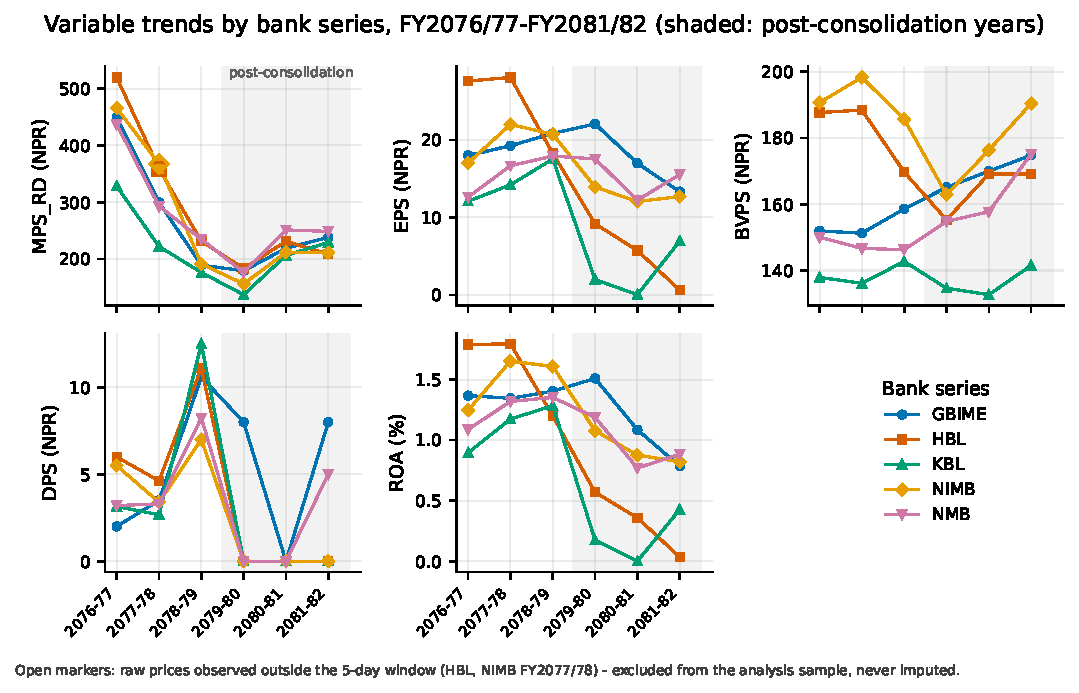
\includegraphics[width=0.92\textwidth]{figures/F6_trends.pdf}
\caption{Variable Trends by Bank Series across FY 2076/77--FY 2081/82}
\label{fig:trends}
\vspace{2pt}
\begin{minipage}{\linewidth}
\footnotesize
\textit{Note.} Variable trends across the six fiscal years (FY 2076/77 through FY 2081/82) for Global IME Bank Limited (GBIME), Himalayan Bank Limited (HBL), Kumari Bank Limited (KBL), Nepal Investment Mega Bank Limited (NIMB), and NMB Bank Limited (NMB). The shaded region delineates the post-consolidation regime (FY 2079/80--FY 2081/82). Window-excluded prices for HBL and NIMB in FY 2077/78 are represented as open markers. The connecting lines pass continuously through the excluded periods; the open markers designate observations excluded from regression estimation under the freshness rule (Codebase Asset F6).
\end{minipage}
\end{figure}

As visually depicted in Figure~\ref{fig:trends}, the post-consolidation shaded window coincides with a synchronized contraction in market share prices ($\mathit{MPS}^{RD}$), a steep downward break in earnings per share (EPS), and a virtual cessation of dividend payouts (DPS), whereas book value per share (BVPS) remained anchored across the structural divide.

\subsection{Correlation Analysis and Multicollinearity Assessment}
Table~\ref{tab:t2_correlations} reports the Pearson correlation coefficients among the dependent variable and explanatory financial indicators across the 28 realized observations.

\begin{table}[!htbp]
\centering
\small
\caption{Pearson Correlation Matrix of Value-Relevance Variables ($N = 28$)}
\label{tab:t2_correlations}
\begin{tabular}{lccccc}
\toprule
\textbf{Variable} & \textbf{$\mathit{MPS}^{RD}$} & \textbf{EPS} & \textbf{BVPS} & \textbf{DPS} & \textbf{ROA} \\
\midrule
$\mathit{MPS}^{RD}$ & 1.000 &  &  &  &  \\
EPS & 0.358 & 1.000 &  &  &  \\
BVPS & 0.217 & 0.372 & 1.000 &  &  \\
DPS & 0.082 & 0.612\textsuperscript{**} & 0.129 & 1.000 &  \\
ROA & 0.378\textsuperscript{*} & 0.975\textsuperscript{**} & 0.278 & 0.595\textsuperscript{**} & 1.000 \\
\bottomrule
\end{tabular}

\vspace{4pt}
\begin{minipage}{\linewidth}
\footnotesize
\textit{Note.} \textsuperscript{*} $p < 0.05$, \textsuperscript{**} $p < 0.01$ (two-tailed). Analysis sample of 28 realized bank-year observations. Price-to-Earnings (P/E) ratio is excluded by construction due to mechanical endogeneity with Market Price per Share at Reporting Deadline ($\mathit{MPS}^{RD}$).
\end{minipage}
\end{table}

The correlation matrix reveals several key empirical patterns:
\begin{enumerate}
    \item \textbf{Unconditional Price Associations:} In raw, unadjusted bivariate correlations, $\mathit{MPS}^{RD}$ exhibits a positive correlation with EPS ($r = 0.358, p = 0.061$) and BVPS ($r = 0.217, p = 0.268$). Although positive---consistent with general equity valuation logic---neither bivariate association achieves statistical significance at the 5\% level in the unadjusted bivariate sample. Operating profitability (ROA) displays a statistically significant positive bivariate correlation with market price ($r = 0.378, p = 0.047$), whereas cash dividend per share (DPS) exhibits an extraordinarily weak linear correlation ($r = 0.082, p = 0.678$).
    \item \textbf{Severe Collinearity between EPS and ROA:} Crucially, the Pearson correlation coefficient between EPS and ROA is $r = 0.975$ ($p < 0.001$). Entering both regressors simultaneously into a multivariate linear specification would generate severe variance inflation ($\text{VIF} \approx 1 / (1 - 0.975^2) \approx 20.2$), severely destabilizing standard errors, inducing sign reversals, and invalidating inference. Consequently, ROA is strictly excluded from concurrent inclusion with EPS in all econometric specifications; it is deployed exclusively as a substitute operating profitability regressor in robustness specification R3.
    \item \textbf{Core Regressor Independence:} In contrast, the bivariate correlation between the two core explanatory variables of the Ohlson framework---EPS and BVPS---is moderate ($r = 0.372, p = 0.051$). This demonstrates that earnings and book value capture distinct dimensions of financial performance and equity value, retaining sufficient independent variation for simultaneous estimation without multicollinearity distortion.
\end{enumerate}

Figure~\ref{fig:scatter_matrix} presents the bivariate scatter plot matrix among the primary value-relevance variables ($\mathit{MPS}^{RD}$, EPS, and BVPS), while Figure~\ref{fig:heatmap} illustrates the corresponding correlation heatmap.

\begin{figure}[!htbp]
\centering
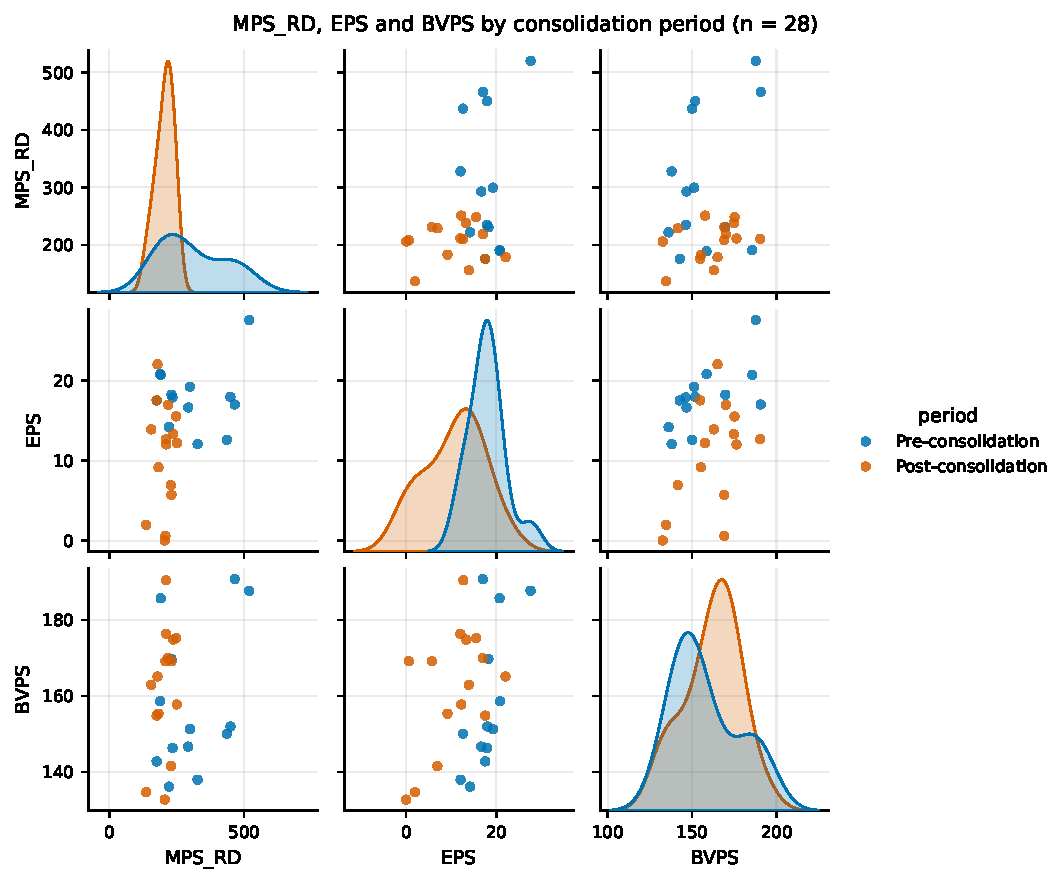
\includegraphics[width=0.88\textwidth]{figures/F1_scatter_matrix.pdf}
\caption{Bivariate Scatter Plot Matrix of Value-Relevance Variables}
\label{fig:scatter_matrix}
\vspace{2pt}
\begin{minipage}{\linewidth}
\footnotesize
\textit{Note.} Pairwise scatter plots and univariate kernel density distributions for $\mathit{MPS}^{RD}$, EPS, and BVPS across the realized panel ($N = 28$) (Codebase Asset F1).
\end{minipage}
\end{figure}

\begin{figure}[!htbp]
\centering
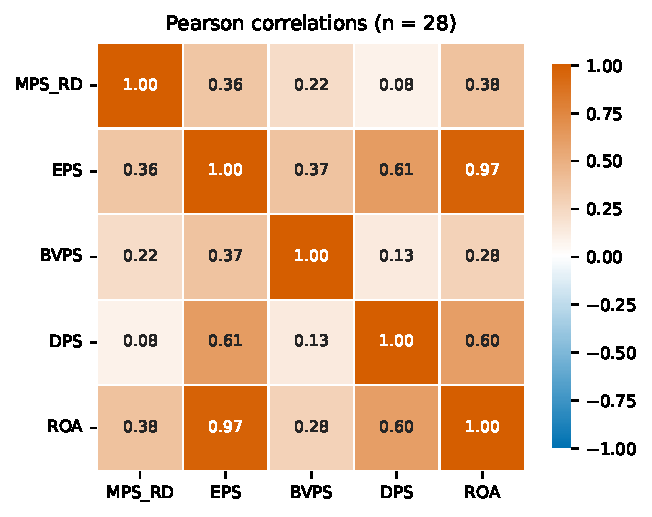
\includegraphics[width=0.72\textwidth]{figures/F2_correlation_heatmap.pdf}
\caption{Pearson Correlation Heatmap of Value-Relevance Variables}
\label{fig:heatmap}
\vspace{2pt}
\begin{minipage}{\linewidth}
\footnotesize
\textit{Note.} Correlation heatmap displaying pairwise Pearson correlation coefficients among value-relevance variables across the realized panel ($N = 28$) (Codebase Asset F2).
\end{minipage}
\end{figure}

\subsection{Baseline Value Relevance: Model 1 Estimation}
To address Research Question~1 and provide an empirical benchmark of accounting value relevance prior to evaluating regime shifts, Model~1 estimates the static Ohlson valuation equation across the entire six-year panel:
\begin{equation}
\mathit{MPS}^{RD}_{it} = \alpha + \mu_i + \lambda_t + \beta_E \mathit{EPS}_{it} + \beta_B \mathit{BVPS}_{it} + \varepsilon_{it}
\end{equation}
where $\alpha$ is the constant baseline intercept, $\mu_i$ represents unobserved time-invariant bank fixed effects (with GBIME serving as reference bank), and $\lambda_t$ represents common fiscal-year fixed effects (with FY 2076/77 serving as reference year). Standard errors, $t$-statistics, $p$-values, and confidence intervals are estimated using \citet{mackinnon1985} HC3 heteroskedasticity-consistent standard errors evaluated on Student's $t$ distribution with residual degrees of freedom ($\text{df} = 16$).

Table~\ref{tab:t3_model1} reports the parameter estimates for Model~1, with MacKinnon-White HC3 robust standard errors in parentheses beneath each estimate; $t$-statistics, $p$-values, and 95\% confidence intervals are reported in the text.

\begin{table}[!htbp]
\centering
\small
\caption{Model 1: Baseline Value Relevance of Accounting Fundamentals ($N = 28$)}
\label{tab:t3_model1}
\begin{tabular}{>{\raggedright\arraybackslash}p{0.38\textwidth}>{\raggedleft\arraybackslash}p{0.32\textwidth}}
\toprule
\textbf{Independent Variable} & \textbf{Dependent Variable: $\mathit{MPS}^{RD}$} \\
\midrule
Earnings per Share (EPS) & 2.095 \\
& (4.096) \\
Book Value per Share (BVPS) & 0.219 \\
& (1.858) \\
\addlinespace
\multicolumn{2}{l}{\textbf{Fixed Effects}} \\
\addlinespace
Bank Fixed Effects ($\mu_i$) & Yes \\
Fiscal-Year Fixed Effects ($\lambda_t$) & Yes \\
\addlinespace
\multicolumn{2}{l}{\textbf{Model Diagnostics}} \\
\addlinespace
Observations ($N$) & 28 \\
$R^2$ (LSDV) & 0.948 \\
Adjusted $R^2$ & 0.912 \\
Within-$R^2$ & 0.152 \\
Residual Degrees of Freedom & 16 \\
\bottomrule
\end{tabular}

\vspace{4pt}
\begin{minipage}{\linewidth}
\footnotesize
\textit{Note.} Dependent variable: Market Price per Share at Reporting Deadline ($\mathit{MPS}^{RD}$). OLS estimation with two-way fixed effects (bank dummies and fiscal-year dummies). MacKinnon-White HC3 robust standard errors in parentheses beneath parameter estimates. Bank fixed effects include 4 dummies (reference: GBIME); fiscal-year fixed effects include 5 dummies (reference: FY 2076/77). $R^2$ (LSDV) is the least-squares dummy-variable fit including fixed effects; Within-$R^2$ is the share of bank-and-year-adjusted variation explained by the slopes. Parameter count: 1 intercept + 4 bank dummies + 5 year dummies + 2 slopes = 12 parameters; residual degrees of freedom: $28 - 12 = 16$. Two-tailed tests at 5\% significance level; $t$-statistics, $p$-values, and 95\% confidence intervals are reported in the text.
\end{minipage}
\end{table}

The baseline results in Table~\ref{tab:t3_model1} provide important empirical insights:
\begin{enumerate}
    \item \textbf{Coefficient Magnitudes and Signs:} Both accounting fundamentals exhibit positive coefficients: $\beta_E = 2.095$ and $\beta_B = 0.219$. In economic terms, this suggests that across the full observation span, each additional NPR 1.00 of reported earnings per share is associated with an incremental NPR 2.10 in post-deadline market share price, while each additional NPR 1.00 of book equity per share is associated with an incremental NPR 0.22 in market price, holding unobserved bank characteristics and common macro-temporal shocks constant.
    \item \textbf{Statistical Significance under Robust Inference:} Neither slope coefficient achieves statistical significance at conventional levels. For EPS, the $t$-statistic is $0.51$ ($p = 0.616$ on $t(16)$), and the 95\% HC3 confidence interval spans widely from NPR $-6.587$ to NPR $10.777$. For BVPS, the $t$-statistic is $0.12$ ($p = 0.908$ on $t(16)$), with a 95\% confidence interval spanning from NPR $-3.720$ to NPR $4.158$.
    \item \textbf{Goodness of Fit and Degrees of Freedom:} The model exhibits a high coefficient of determination ($R^2 = 0.948$, Adjusted $R^2 = 0.912$). However, as demonstrated in the specification comparisons in Section~4.2.7, this high explanatory power is almost entirely driven by the two-way fixed effects structure---specifically the fiscal-year dummies ($\lambda_t$), which absorb the substantial macro-market repricing of NEPSE over this period. Accounting for 1 constant intercept, 4 bank dummy parameters, 5 fiscal-year dummy parameters, and 2 slope regressors consumes 12 degrees of freedom, leaving exactly $28 - 12 = 16$ residual degrees of freedom.
\end{enumerate}

\subsection{Impact of Consolidation on Value Relevance: Model 2 Estimation}
To evaluate Research Question~2 and directly test whether the 2023 consolidation wave altered the valuation relationship between accounting fundamentals and equity prices, Model~2 introduces consolidation interaction terms into the two-way fixed effects framework:
\begin{equation}
\begin{aligned}
\mathit{MPS}^{RD}_{it} ={}& \alpha + \mu_i + \lambda_t + \beta_E \mathit{EPS}_{it} + \beta_B \mathit{BVPS}_{it} \\
& + \delta_E (\mathit{EPS}_{it} \times \mathit{Post}_t) + \delta_B (\mathit{BVPS}_{it} \times \mathit{Post}_t) + \varepsilon_{it}
\end{aligned}
\end{equation}
where $\mathit{Post}_t = 1$ for the post-consolidation fiscal years (FY 2079/80, 2080/81, and 2081/82) and $\mathit{Post}_t = 0$ for the pre-consolidation fiscal years (FY 2076/77, 2077/78, and 2078/79). Reference categories remain identical (GBIME for $\mu_i$, FY 2076/77 for $\lambda_t$).

Because common fiscal-year fixed effects ($\lambda_t$) are fully specified, the stand-alone indicator $\mathit{Post}_t$ is an exact linear combination of the fiscal-year dummies ($\mathit{Post}_t = D_{2079/80} + D_{2080/81} + D_{2081/82}$); consequently, the main effect of $\mathit{Post}_t$ is perfectly absorbed by the year fixed effects and cannot be separately estimated. The pre-consolidation valuation slopes are captured by $\beta_E$ and $\beta_B$, the regime interaction coefficients are captured by $\delta_E$ and $\delta_B$, and the implied post-consolidation valuation slopes are given by the linear combinations $(\beta_E + \delta_E)$ and $(\beta_B + \delta_B)$.

Table~\ref{tab:t4_model2} reports the estimation results for Model~2, including pre-consolidation slopes, interaction shifts, implied post-consolidation slopes, and the principal joint Wald test of structural parameter change, with MacKinnon-White HC3 robust standard errors in parentheses beneath each estimate on Student's $t$ distribution ($\text{df} = 14$); $t$-statistics, $p$-values, and confidence intervals are reported in the text.

\begin{table}[!htbp]
\centering
\small
\caption{Model 2: Value Relevance Regime Shift Across Consolidation ($N = 28$)}
\label{tab:t4_model2}
\begin{tabular}{>{\raggedright\arraybackslash}p{0.38\textwidth}>{\raggedleft\arraybackslash}p{0.32\textwidth}}
\toprule
\textbf{Model Parameter / Term} & \textbf{Dependent Variable: $\mathit{MPS}^{RD}$} \\
\midrule
\multicolumn{2}{l}{\textbf{Pre-Consolidation Slopes}} \\
\addlinespace
Earnings per Share ($\beta_E$) & 5.577 \\
& (3.560) \\
Book Value per Share ($\beta_B$) & 0.100 \\
& (1.306) \\
\addlinespace
\multicolumn{2}{l}{\textbf{Consolidation Interaction Shifts}} \\
\addlinespace
EPS $\times$ Post ($\delta_E$) & $-3.124$ \\
& (4.003) \\
BVPS $\times$ Post ($\delta_B$) & $-1.758$ \\
& (1.231) \\
\addlinespace
\multicolumn{2}{l}{\textbf{Implied Post-Consolidation Slopes}} \\
\addlinespace
Implied EPS Slope ($\beta_E + \delta_E$) & 2.453 \\
& (2.269) \\
Implied BVPS Slope ($\beta_B + \delta_B$) & $-1.658$ \\
& (1.120) \\
\addlinespace
\multicolumn{2}{l}{\textbf{Diagnostics and Structural Change Tests}} \\
\addlinespace
Wald Test: $F(2, 14)$ \newline $[H_0: \delta_E = \delta_B = 0]$ & 2.954 ($p = 0.085$) \\
Bank Fixed Effects ($\mu_i$) & Yes \\
Fiscal-Year Fixed Effects ($\lambda_t$) & Yes \\
Observations ($N$) & 28 \\
$R^2$ (LSDV) & 0.978 \\
Within-$R^2$ & 0.642 \\
Residual Degrees of Freedom & 14 \\
\bottomrule
\end{tabular}

\vspace{4pt}
\begin{minipage}{\linewidth}
\footnotesize
\textit{Note.} Dependent variable: $\mathit{MPS}^{RD}$. OLS estimation with bank and fiscal-year fixed effects. Post indicator equals 1 for FY 2079/80--2081/82 and 0 for FY 2076/77--2078/79; stand-alone Post main effect is fully absorbed by the fiscal-year fixed effects. MacKinnon-White HC3 robust standard errors in parentheses beneath parameter estimates. Bank fixed effects include 4 dummies (reference: GBIME); fiscal-year fixed effects include 5 dummies (reference: FY 2076/77). $R^2$ (LSDV) is the least-squares dummy-variable fit including fixed effects; Within-$R^2$ is the share of bank-and-year-adjusted variation explained by the slopes and interactions. Implied post-consolidation slopes are linear combinations evaluated under the HC3 covariance. Residual degrees of freedom: $28 - 14 = 14$. Two-tailed $t$-tests for individual parameters; right-tail Wald $F$-test for joint hypothesis; the Wald test is marginally significant at the 10\% level. $t$-statistics, $p$-values, and confidence intervals are reported in the text.
\end{minipage}
\end{table}

The empirical estimates in Table~\ref{tab:t4_model2} provide substantive evidence regarding structural changes in valuation dynamics:
\begin{enumerate}
    \item \textbf{Pre-Consolidation Valuation Regime:}
    \begin{itemize}
        \item Prior to the 2023 consolidation wave, the estimated valuation slope for earnings per share was $\beta_E = 5.577$ (HC3 SE = 3.560, $t = 1.57, p = 0.140$). In economic magnitude, equity investors priced commercial bank shares at approximately 5.58 times reported earnings per share. While economically substantial, this estimate is not statistically significant at the 5\% level ($p = 0.140$ on $t(14)$), reflecting the wide confidence interval ([-2.059, 13.213]) resulting from small sample degrees of freedom and conservative HC3 standard errors.
        \item The pre-consolidation slope for book value per share was negligible: $\beta_B = 0.100$ (HC3 SE = 1.306, $t = 0.08, p = 0.940$). In the pre-consolidation environment, secondary market share prices were predominantly driven by earnings and dividend capacity rather than balance-sheet equity backing.
    \end{itemize}
    \item \textbf{Consolidation Regime Interaction Shifts:}
    \begin{itemize}
        \item The earnings interaction coefficient is negative: $\delta_E = -3.124$ (HC3 SE = 4.003, $t = -0.78, p = 0.448$). Although statistically insignificant in isolation ($p = 0.448$), the point estimate indicates that post-consolidation equity prices discounted reported earnings by approximately NPR 3.12 per rupee of EPS relative to the pre-consolidation regime, cutting the implied earnings multiple by more than half.
        \item The book value interaction coefficient is also negative: $\delta_B = -1.758$ (HC3 SE = 1.231, $t = -1.43, p = 0.175$). While not statistically significant at the 5\% level ($p = 0.175$), the point estimate reflects an erosion of the valuation multiple attached to book equity by NPR 1.76 per rupee of BVPS.
    \end{itemize}
    \item \textbf{Implied Post-Consolidation Slopes:}
    \begin{itemize}
        \item Combining the baseline slope and interaction shift yields an implied post-consolidation earnings slope of $\beta_E + \delta_E = 2.453$ (HC3 SE = 2.269, $t = 1.08, p = 0.298$). The pricing of earnings compressed from 5.58 times EPS to 2.45 times EPS.
        \item For book value, the implied post-consolidation slope is negative: $\beta_B + \delta_B = -1.658$ (HC3 SE = 1.120, $t = -1.48, p = 0.161$). Rather than serving as an asset anchor, increases in book equity following the merger wave were weakly associated with lower share prices, reflecting market apprehension over asset quality dilution, goodwill recognition, and capital overhang.
    \end{itemize}
    \item \textbf{Principal Joint Wald Test of Regime Shift:}
    \begin{itemize}
        \item Because corporate combinations simultaneously alter multiple accounting dimensions, testing interaction coefficients individually can fail to capture multi-parameter structural shifts. The principal econometric test is the joint Wald $F$-test evaluating the composite null hypothesis that both interaction terms are simultaneously zero ($H_0: \delta_E = 0 \text{ and } \delta_B = 0$).
        \item The joint test yields $F(2, 14) = 2.954$ with an $F$-distribution $p$-value of $0.085$. Under the designated 5\% significance threshold, the null hypothesis of structural stability cannot be rejected ($p = 0.085 > 0.05$). However, the joint test achieves marginal significance at the 10\% level ($p < 0.10$), providing suggestive evidence of a joint structural shift in the accounting valuation function.
    \end{itemize}
    \item \textbf{Parameter Accounting and Residual Degrees of Freedom:}
    Model~2 estimates 1 constant intercept, 4 bank fixed effects (GBIME reference), 5 fiscal-year fixed effects (FY 2076/77 reference), 2 main slope parameters ($\beta_E, \beta_B$), and 2 interaction parameters ($\delta_E, \delta_B$), consuming a total of 14 degrees of freedom. On $N = 28$ observations, this leaves exactly $28 - 14 = 14$ residual degrees of freedom.
\end{enumerate}

To visually display these pre- and post-consolidation relationships, Figure~\ref{fig:value_relevance} presents bivariate scatter plots of $\mathit{MPS}^{RD}$ against EPS and BVPS partitioned by consolidation regime, while Figure~\ref{fig:coeff_forest} presents the coefficient forest plot for Model~2.

\begin{figure}[!htbp]
\centering
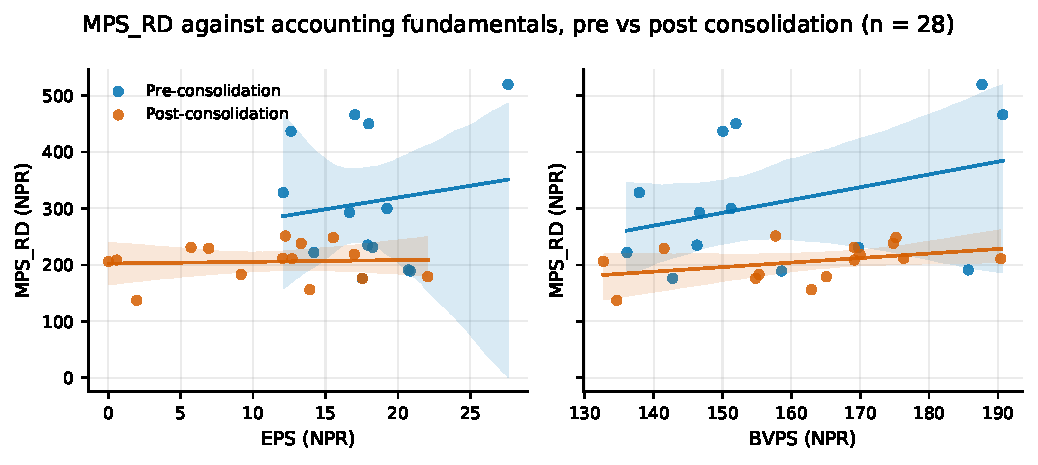
\includegraphics[width=0.92\textwidth]{figures/F3_value_relevance.pdf}
\caption{$\mathit{MPS}^{RD}$ against Fundamentals Pre vs.\ Post Consolidation}
\label{fig:value_relevance}
\vspace{2pt}
\begin{minipage}{\linewidth}
\footnotesize
\textit{Note.} Scatter panels and OLS regression lines of $\mathit{MPS}^{RD}$ against EPS (left) and BVPS (right), partitioned into pre-consolidation (FY 2076/77--2078/79, blue) and post-consolidation (FY 2079/80--2081/82, vermillion) sub-periods ($N = 28$) (Codebase Asset F3). Lines are descriptive bivariate OLS fits, not the two-way fixed-effects estimates in Table~\ref{tab:t4_model2}; the post-BVPS sign difference is the effect of absorbing year effects.
\end{minipage}
\end{figure}

\begin{figure}[!htbp]
\centering
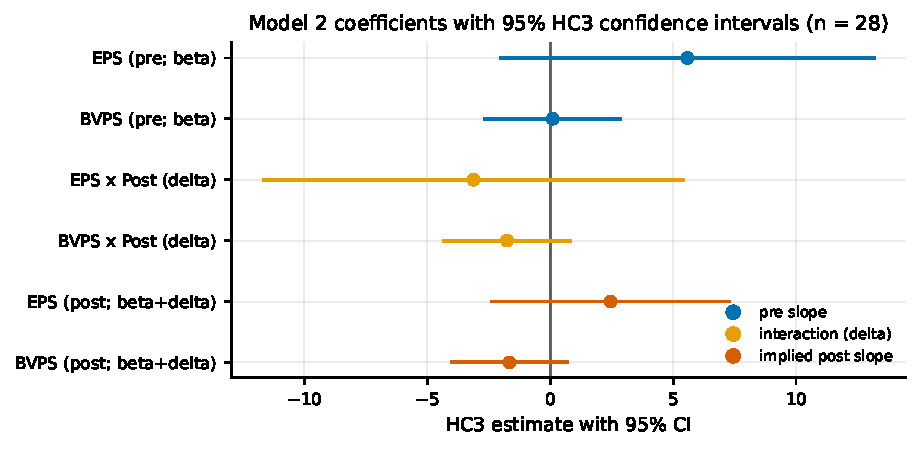
\includegraphics[width=0.88\textwidth]{figures/F4_coefficient_forest.pdf}
\caption{Model 2 Coefficients and 95\% HC3 Confidence Intervals}
\label{fig:coeff_forest}
\vspace{2pt}
\begin{minipage}{\linewidth}
\footnotesize
\textit{Note.} Coefficient forest plot displaying pre-consolidation slopes ($\beta_E, \beta_B$), interaction shifts ($\delta_E, \delta_B$), and implied post-consolidation linear combinations ($\beta_E+\delta_E, \beta_B+\delta_B$) from Model~2, estimated with MacKinnon-White HC3 robust 95\% confidence intervals on Student's $t(14)$ distribution ($N = 28, \text{residual df} = 14$) (Codebase Asset F4).
\end{minipage}
\end{figure}

\subsection{Hypothesis Testing}
Based on the econometric estimates obtained from Model~1 and Model~2, the four operational research hypotheses formulated in Chapter~I are formally evaluated at the designated two-tailed 5\% significance level ($\alpha = 0.05$).

To ensure rigorous transparency, Hypotheses $H_1$ and $H_2$ are evaluated under both Model~1 (overall six-year baseline slopes) and Model~2 (pre-consolidation regime slopes). In both specifications, the empirical decision is identical.

Table~\ref{tab:hypotheses} summarizes the formal hypothesis testing decisions.

\begin{table}[!htbp]
\centering
\small
\caption{Summary of Operational Hypothesis Testing Decisions}
\label{tab:hypotheses}
\begin{tabular}{>{\raggedright\arraybackslash}p{0.125\textwidth}>{\raggedright\arraybackslash}p{0.11\textwidth}>{\raggedright\arraybackslash}p{0.11\textwidth}cc>{\raggedright\arraybackslash}p{0.11\textwidth}>{\raggedright\arraybackslash}p{0.18\textwidth}}
\toprule
\textbf{Hypothesis} & \textbf{Model / Term} & \textbf{Null ($H_0$)} & \textbf{Estimate} & \textbf{$p$-value} & \textbf{Decision} & \textbf{Inference} \\
\midrule
$H_1$ (Model 1) & $\beta_E$ (Overall) & $\beta_E = 0$ & 2.095 & 0.616 & Fail to Reject & Positive slope; insignificant under $t(16)$. \\
\addlinespace
$H_1$ (Model 2) & $\beta_E$ (Pre Slope) & $\beta_E = 0$ & 5.577 & 0.140 & Fail to Reject & Substantial slope; insignificant at 5\% ($t(14)$). \\
\addlinespace
$H_2$ (Model 1) & $\beta_B$ (Overall) & $\beta_B = 0$ & 0.219 & 0.908 & Fail to Reject & Insignificant under $t(16)$. \\
\addlinespace
$H_2$ (Model 2) & $\beta_B$ (Pre Slope) & $\beta_B = 0$ & 0.100 & 0.940 & Fail to Reject & Indistinguishable from zero under $t(14)$. \\
\addlinespace
$H_3$ & $\delta_E$ (EPS Shift) & $\delta_E = 0$ & $-3.124$ & 0.448 & Fail to Reject & Downward shift; insignificant under $t(14)$. \\
\addlinespace
$H_4$ & $\delta_B$ (BVPS Shift) & $\delta_B = 0$ & $-1.758$ & 0.175 & Fail to Reject & Downward shift; insignificant under $t(14)$. \\
\addlinespace
Joint Test & Joint Wald & $\delta_E=\delta_B=0$ & $F=2.95$ & 0.085 & Fail to Reject & Marginal at 10\%; fails 5\% threshold. \\
\bottomrule
\end{tabular}

\vspace{4pt}
\begin{minipage}{\linewidth}
\footnotesize
\textit{Note.} All tests evaluated at $\alpha = 0.05$ (two-tailed $t$-tests for individual parameters; right-tail $F$-test for joint hypothesis). Estimates derived from Model~1 ($N = 28, \text{residual df} = 16$) and Model~2 ($N = 28, \text{residual df} = 14$) with two-way fixed effects and MacKinnon-White HC3 robust standard errors on Student's $t$ distribution.
\end{minipage}
\end{table}

Detailed evaluations of individual hypotheses:
\begin{enumerate}
    \item \textbf{Hypothesis 1 ($H_1$): Value Relevance of Earnings per Share:}
    \textit{Hypothesis Statement:} There is a statistically significant relationship between earnings per share and market share price ($H_0: \beta_E = 0$ vs.\ $H_1: \beta_E \ne 0$).
    In Model~1, the overall EPS slope is $\hat{\beta}_E = 2.095$ with an HC3 standard error of $4.096$ ($t = 0.51, p = 0.616$). In Model~2, the pre-consolidation EPS slope is estimated at $\hat{\beta}_E = 5.577$ with an HC3 standard error of $3.560$ ($t = 1.57, p = 0.140$). In both models, the point estimates are positive and economically meaningful, but because $p > 0.05$, the study fails to reject the null hypothesis of no statistical association at the 5\% significance level.
    \item \textbf{Hypothesis 2 ($H_2$): Value Relevance of Book Value per Share:}
    \textit{Hypothesis Statement:} There is a statistically significant relationship between book value per share and market share price ($H_0: \beta_B = 0$ vs.\ $H_1: \beta_B \ne 0$).
    In Model~1, the overall slope is $\hat{\beta}_B = 0.219$ ($t = 0.12, p = 0.908$). In Model~2, the pre-consolidation BVPS slope is $\hat{\beta}_B = 0.100$ with an HC3 standard error of $1.306$ ($t = 0.08, p = 0.940$). Because $p \gg 0.05$ across both specifications, the study fails to reject the null hypothesis. Prior to consolidation, book value per share provided negligible explanatory power for share prices beyond earnings and fixed effects.
    \item \textbf{Hypothesis 3 ($H_3$): Structural Shift in Earnings Value Relevance:}
    \textit{Hypothesis Statement:} The value relevance of earnings per share underwent a statistically significant shift following the 2023 consolidation wave ($H_0: \delta_E = 0$ vs.\ $H_1: \delta_E \ne 0$).
    The interaction coefficient is $\hat{\delta}_E = -3.124$ with an HC3 standard error of $4.003$ ($t = -0.78, p = 0.448$). Although the point estimate indicates a substantial downward shift in the valuation multiple, the individual coefficient is not statistically significant at conventional thresholds. The study fails to reject the null hypothesis of no structural shift in EPS value relevance when evaluated in isolation.
    \item \textbf{Hypothesis 4 ($H_4$): Structural Shift in Book Value Relevance:}
    \textit{Hypothesis Statement:} The value relevance of book value per share underwent a statistically significant shift following the 2023 consolidation wave ($H_0: \delta_B = 0$ vs.\ $H_1: \delta_B \ne 0$).
    The interaction coefficient is $\hat{\delta}_B = -1.758$ with an HC3 standard error of $1.231$ ($t = -1.43, p = 0.175$). Although the negative shift reduces the implied post-consolidation slope to $-1.658$, the interaction term does not achieve statistical significance at the 5\% level. The study fails to reject the null hypothesis of no structural shift in BVPS value relevance when evaluated in isolation.
    \item \textbf{Principal Joint Structural Test:}
    Evaluating the joint composite hypothesis $H_0: \delta_E = \delta_B = 0$ yields $F(2, 14) = 2.954$ ($p = 0.085$). While the study cannot reject the null hypothesis of parameter stability at the strict 5\% level, the marginal significance ($p < 0.10$) is consistent with non-trivial joint adjustments across accounting valuation multiples.
\end{enumerate}

\subsection{Robustness and Sensitivity Analyses (R1 through R8)}
To evaluate the stability of baseline estimates against alternative empirical assumptions, variable definitions, and sample compositions, an eight-specification suite comprising the two baseline models (R1--R2) and six robustness variants (R3--R8) was estimated. All specifications maintain two-way bank and fiscal-year fixed effects and MacKinnon-White HC3 robust inference on Student's $t$ residual degrees of freedom.

Table~\ref{tab:t5_robustness} summarizes the estimation results across the robustness suite, reporting point estimates, standard errors for both main slopes and interaction terms, and the joint Wald $F$-test.

\begin{table}[!htbp]
\centering
\small
\caption{Robustness and Sensitivity Analysis Across Econometric Specifications}
\label{tab:t5_robustness}
\setlength{\tabcolsep}{4pt}
\begin{tabular}{>{\raggedright\arraybackslash}p{0.19\textwidth}>{\raggedright\arraybackslash}p{0.13\textwidth}>{\raggedright\arraybackslash}p{0.12\textwidth}>{\raggedright\arraybackslash}p{0.14\textwidth}>{\raggedright\arraybackslash}p{0.12\textwidth}>{\raggedright\arraybackslash}p{0.12\textwidth}c}
\toprule
\textbf{Specification} & \textbf{Earnings (SE)} & \textbf{BVPS (SE)} & \textbf{$\delta_E$ (SE)} & \textbf{$\delta_B$ (SE)} & \textbf{Wald $F$ ($p$)} & \textbf{$n$} \\
\midrule
\textbf{R1:} Model 1 Baseline & 2.095 (4.096) & 0.219 (1.858) & --- & --- & --- & 28 \\
\addlinespace
\textbf{R2:} Model 2 Baseline & 5.577 (3.560) & 0.100 (1.306) & $-3.124$ (4.003) & $-1.758$ (1.231) & 2.95 (0.085) & 28 \\
\addlinespace
\textbf{R3:} ROA Replaces EPS & 83.760 (79.852) & 0.358 (1.381) & $-43.570$ (83.671) & $-1.901$ (1.290) & 2.46 (0.121) & 28 \\
\addlinespace
\textbf{R4:} Model 2 + DPS & 6.183 (4.508) & $-0.642$ (1.378) & $-4.072$ (5.151) & $-1.770$ (1.335) & 2.77 (0.100) & 28 \\
\addlinespace
\textbf{R5:} Excl.\ Transition & 5.993 (4.635) & $-0.201$ (1.849) & $-2.578$ (5.521) & $-1.880$ (1.419) & 2.41 (0.139) & 23 \\
\addlinespace
\textbf{R6:} Excl.\ Mismatch & 4.336 (3.724) & 0.802 (1.328) & $-2.436$ (4.755) & $-2.611$ (1.517) & \textbf{5.82 (0.021)\textsuperscript{*}} & 23 \\
\addlinespace
\textbf{R7:} Bonus-Adjusted & 5.775 (4.145) & 0.153 (1.632) & $-4.043$ (4.446) & $-1.533$ (1.595) & 2.37 (0.130) & 28 \\
\addlinespace
\textbf{R8:} Restated EPS & 5.256 (3.016) & 0.031 (1.300) & $-2.860$ (3.807) & $-1.812$ (1.223) & 2.92 (0.087) & 28 \\
\bottomrule
\end{tabular}

\vspace{4pt}
\begin{minipage}{\linewidth}
\footnotesize
\textit{Note.} \textsuperscript{*} Significant at $p < 0.05$. All models estimated by OLS with bank and fiscal-year fixed effects; MacKinnon-White HC3 robust standard errors reported in parentheses. The joint Wald $F$-statistic tests $H_0: \delta_E = \delta_B = 0$ under the MacKinnon-White HC3 covariance matrix. R3: ROA substitutes for EPS. R4: Cash DPS included (residual df = 13). R5: Transition year FY 2079/80 dropped ($N = 23, \text{residual df} = 10$). R6: FY 2078/79 entity-timing mismatch dropped ($N = 23, \text{residual df} = 10$). R7: BVPS adjusted for proposed bonus share capitalization ($\mathit{BVPS}_{\text{adj}} = \mathit{BVPS} / (1 + \text{bonus ratio})$, a pro-forma forward capitalization adjustment). R8: Restated basic EPS substituted for GBIME FY 2076/77 and NMB FY 2077/78 ($N = 28$). Residual degrees of freedom: R1 16; R2, R3, R7, R8 14; R4 13; R5, R6 10.
\end{minipage}
\end{table}

The sensitivity analysis yields critical econometric and substantive insights:
\begin{enumerate}
    \item \textbf{Operating Profitability Substitution (R3):} Substituting ROA (PAT divided by average total assets) for EPS yields an operating profitability slope of $83.760$ (HC3 SE = 79.852, $p = 0.312$) and an interaction shift of $\delta_{ROA} = -43.570$ (HC3 SE = 83.671, $p = 0.611$). The book value interaction remains negative ($\delta_B = -1.901, \text{SE} = 1.290, p = 0.163$), and the joint Wald test yields $F(2, 14) = 2.46$ ($p = 0.121$). This confirms that the observed valuation dynamics are not an artifact of per-share earnings scaling, but reflect fundamental operational repricing.
    \item \textbf{Dividend Incorporation (R4):} Augmenting Model~2 with declared cash dividends per share (DPS) produces an earnings slope of $\hat{\beta}_E = 6.183$ (SE = 4.508, $p = 0.193$) and a book value slope of $\hat{\beta}_B = -0.642$ (SE = 1.378, $p = 0.649$). The interaction shifts remain consistently negative ($\delta_E = -4.072, \text{SE} = 5.151, p = 0.443; \delta_B = -1.770, \text{SE} = 1.335, p = 0.208$), and the joint Wald $F$ is $2.77$ ($p = 0.100$). Because adding DPS consumes an additional parameter, residual degrees of freedom decrease from 14 to exactly 13 on $N = 28$.
    \item \textbf{Transition-Year Exclusion (R5):} Dropping the initial post-merger integration year (FY 2079/80, $N = 23, \text{residual df} = 10$) to eliminate one-off transition accounting friction preserves the structural pattern: $\hat{\beta}_E = 5.993$ (SE = 4.635, $p = 0.225$), $\hat{\delta}_E = -2.578$ (SE = 5.521, $p = 0.650$), $\hat{\delta}_B = -1.880$ (SE = 1.419, $p = 0.215$), with joint Wald $F(2, 10) = 2.41$ ($p = 0.139$). This pattern is consistent with the interpretation that the negative interaction shifts are not solely driven by temporary integration write-offs in the immediate post-merger fiscal year.
    \item \textbf{Entity-Timing Mismatch Exclusion (R6) --- Key Sensitivity Finding:} Specification R6 excludes FY 2078/79 ($N = 23, \text{residual df} = 10$). As established in Chapter~III, FY 2078/79 represents an entity-timing asymmetry: audited financial statements published at the end of Chaitra 2079 BS reflected standalone, pre-merger banking operations (ending mid-July 2022), whereas secondary market share prices observed on 13 April 2023 reflected the expanded, post-merger capitalized entities following early-2023 amalgamations.
    When this entity-mismatch fiscal year is excluded, the joint Wald test of regime shift becomes \textbf{statistically significant at the 5\% level}: \textbf{$F(2, 10) = 5.82, p = 0.021$}.
    In this FY 2078/79-excluded specification, the book value interaction shift is estimated at $\hat{\delta}_B = -2.611$ with an HC3 standard error of $1.517$ ($t = -1.72, p = 0.116$ on $t(10)$), while the earnings interaction is $\hat{\delta}_E = -2.436$ (HC3 SE = 4.755, $t = -0.51, p = 0.620$). While neither individual interaction term achieves significance at the 10\% level under the Student's $t(10)$ distribution, the joint test indicates that removing the entity-timing asymmetry yields a statistically significant joint structural difference across the pre- and post-consolidation calendar regimes.
    \item \textbf{Bonus Capitalization Adjustment (R7):} Adjusting book value for subsequent bonus share dilution ($\mathit{BVPS}_{\text{adj}} = \mathit{BVPS} / (1 + \text{bonus ratio})$) yields estimates virtually identical to baseline: $\hat{\beta}_E = 5.775$ (SE = 4.145, $p = 0.185$), $\hat{\delta}_E = -4.043$ (SE = 4.446, $p = 0.379$), $\hat{\delta}_B = -1.533$ (SE = 1.595, $p = 0.353$), with Wald $F(2, 14) = 2.37$ ($p = 0.130$).
    \item \textbf{Restated Earnings per Share (R8):} Substituting restated basic EPS (accounting for bonus issues in subsequent fiscal periods for GBIME FY 2076/77 and NMB FY 2077/78) leaves the baseline conclusions intact: $\hat{\beta}_E = 5.256$ (SE = 3.016, $p = 0.103$), $\hat{\delta}_E = -2.860$ (SE = 3.807, $p = 0.465$), $\hat{\delta}_B = -1.812$ (SE = 1.223, $p = 0.161$), with Wald $F(2, 14) = 2.92$ ($p = 0.087$).
\end{enumerate}

Figure~\ref{fig:robustness_forest} presents a coefficient forest plot summarizing parameter estimates and confidence intervals for the earnings channel across seven robustness specifications (R1, R2, and R4 through R8).

\begin{figure}[!htbp]
\centering
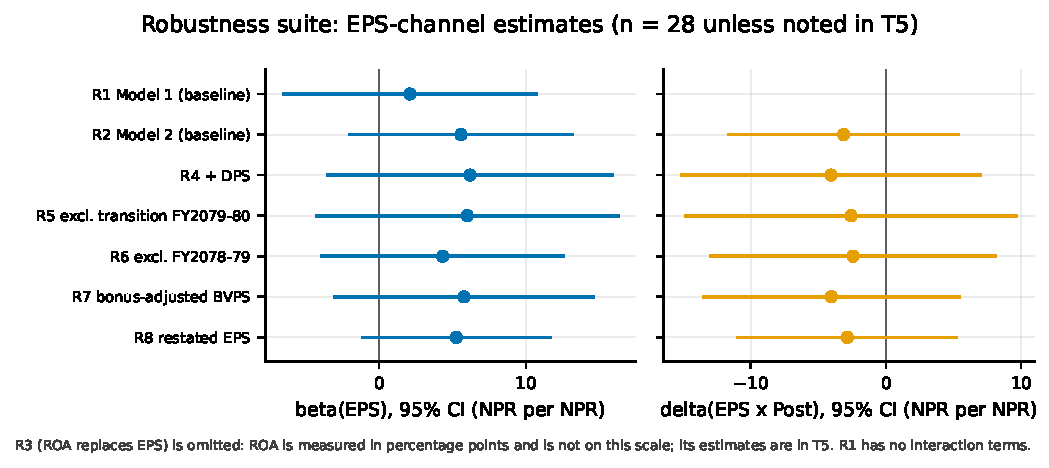
\includegraphics[width=0.92\textwidth]{figures/A2_robustness_forest.pdf}
\caption{Robustness Forest Plot Across Seven Specifications (R1, R2, R4--R8)}
\label{fig:robustness_forest}
\vspace{2pt}
\begin{minipage}{\linewidth}
\footnotesize
\textit{Note.} Forest plot of the EPS-channel estimates (earnings coefficient and EPS $\times$ Post interaction) with 95\% HC3 confidence intervals across seven specifications (R1, R2, R4--R8; R3 omitted because ROA is on a different scale; $N = 28$ or $N = 23$) (Codebase Asset A2).
\end{minipage}
\end{figure}

\subsection{Econometric Diagnostics and Specification Comparison}
To verify that the empirical findings are robust to potential violations of Gauss-Markov and asymptotic assumptions, a comprehensive battery of econometric diagnostics was performed.

Table~\ref{tab:t6_diagnostics} presents the diagnostic test statistics for the baseline model.

\begin{table}[!htbp]
\centering
\small
\caption{Econometric Diagnostics for Baseline Value-Relevance Model}
\label{tab:t6_diagnostics}
\begin{tabular}{>{\raggedright\arraybackslash}p{0.22\textwidth}cccc}
\toprule
\textbf{Diagnostic Dimension} & \textbf{Statistic} & \textbf{Value} & \textbf{$p$-value / Threshold} & \textbf{Assessment} \\
\midrule
VIF (EPS) & VIF & 1.16 & $< 10.0$ (Tolerance = 0.862) & Passed \\
\addlinespace
VIF (BVPS) & VIF & 1.16 & $< 10.0$ (Tolerance = 0.862) & Passed \\
\addlinespace
Breusch-Pagan Heteroskedasticity & LM & 14.37 & $p = 0.213$ ($\chi^2(11) = 19.68$) & Passed \\
\addlinespace
Cook's Distance (Influential) & Max $D_i$ & 0.552 & Cutoff: $4/N = 0.143$ & Addressed via HC3 \\
\bottomrule
\end{tabular}

\vspace{4pt}
\begin{minipage}{\linewidth}
\footnotesize
\textit{Note.} Diagnostics computed on Model~1 baseline ($N = 28$). Variance Inflation Factor (VIF) computed exclusively on substantive regressors (fixed effects dummies excluded). Breusch-Pagan Lagrange Multiplier test evaluates residual variance constancy across fitted values and regressors. Cook's distance evaluated using the correct parameter count ($K = 12$) against standard finite-sample threshold $4/N = 4/28 = 0.143$.
\end{minipage}
\end{table}

Key diagnostic findings:
\begin{enumerate}
    \item \textbf{Multicollinearity:} The variance inflation factors for EPS and BVPS are identical at $\text{VIF} = 1.16$ (tolerance = 0.862). Because these values fall well below the conventional conservative ceiling of $5.0$ (and standard threshold of $10.0$), multicollinearity between the substantive accounting fundamentals does not distort parameter estimation.
    \item \textbf{Heteroskedasticity:} The Breusch-Pagan test yields an LM statistic of $14.37$ ($p = 0.213$). Although the null hypothesis of constant error variance is not formally rejected at the 5\% level, all inferences throughout this dissertation are executed under MacKinnon-White HC3 standard errors, which provide asymptotic and finite-sample protection against arbitrary heteroskedasticity and high-leverage points.
    \item \textbf{Influential Observations:} Evaluating Cook's distance against the benchmark threshold $4/N = 4/28 = 0.143$ identifies five observations exceeding the cutoff, with a sample maximum Cook's $D$ of $0.552$ (HBL FY 2076/77). These high-leverage observations correspond to extreme price realizations during the 2021 NEPSE bull market. Deployment of HC3 standard errors explicitly addresses this leverage: the HC3 estimator divides squared residuals by $(1 - h_{ii})^2$, inflating high-leverage residuals to offset their artificially small OLS residuals. This yields conservative standard error estimates and protects inference against leverage distortion, without artificially trimming or modifying observed sample data.
\end{enumerate}

Figure~\ref{fig:diagnostics} presents the four-panel econometric diagnostic plot for Model~1 (Normal Q-Q, Residuals vs.\ Fitted, Scale-Location, and Cook's Distance).

\begin{figure}[!htbp]
\centering
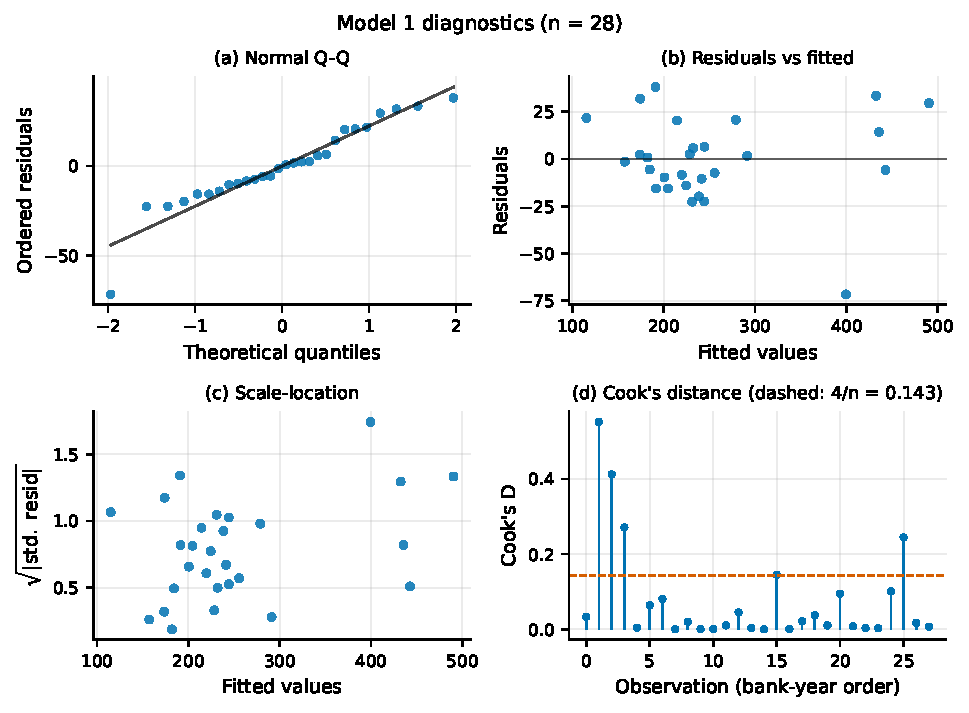
\includegraphics[width=0.92\textwidth]{figures/F5_diagnostics.pdf}
\caption{Econometric Residual Diagnostics for Baseline Model (Model 1)}
\label{fig:diagnostics}
\vspace{2pt}
\begin{minipage}{\linewidth}
\footnotesize
\textit{Note.} Four-panel diagnostic suite for Model~1: (top-left) Normal Q-Q plot assessing error normality; (top-right) Residuals vs.\ Fitted values assessing linearity; (bottom-left) Scale-Location plot ($\sqrt{|\text{standardized residuals}|}$ vs.\ fitted) assessing homoskedasticity; (bottom-right) Cook's distance across observations ($N = 28$) identifying leverage points against $4/N = 0.143$ (Codebase Asset F5).
\end{minipage}
\end{figure}

\subsubsection{Specification Comparison: Pooled OLS vs.\ Fixed Effects}
To demonstrate why two-way fixed effects estimation is the preferred econometric specification, Table~\ref{tab:spec_comp} compares parameter estimates across three nested specifications: Pooled OLS (no fixed effects), Bank Fixed Effects Only, and Two-Way Fixed Effects (Model~1).

\begin{table}[!htbp]
\centering
\small
\caption{Specification Comparison Across Econometric Model Structures}
\label{tab:spec_comp}
\setlength{\tabcolsep}{4pt}
\begin{tabular}{>{\raggedright\arraybackslash}p{0.18\textwidth}cccc>{\raggedright\arraybackslash}p{0.20\textwidth}}
\toprule
\textbf{Specification} & \textbf{$\beta_E$ (EPS Coef.)} & \textbf{$\beta_B$ (BVPS Coef.)} & \textbf{$R^2$} & \textbf{Resid.\ df} & \textbf{Assessment} \\
\midrule
Pooled OLS (No FE) & 4.882 (3.099) & 0.552 (1.259) & 0.136 & 25 & Conflates market cycles with relevance. \\
\addlinespace
Bank FE Only & 5.217 (5.360) & 1.432 (2.727) & 0.176 & 21 & Ignores macro-temporal price collapse. \\
\addlinespace
Two-Way FE (Model 1) & 2.095 (4.096) & 0.219 (1.858) & 0.948 & 16 & Rigorously absorbs bank and year shocks; preferred benchmark. \\
\bottomrule
\end{tabular}

\vspace{4pt}
\begin{minipage}{\linewidth}
\footnotesize
\textit{Note.} MacKinnon-White HC3 robust standard errors reported in parentheses. Dependent variable: $\mathit{MPS}^{RD}$. Analysis sample $N = 28$.
\end{minipage}
\end{table}

The comparison in Table~\ref{tab:spec_comp} reveals that Pooled OLS yields inflated point estimates ($\hat{\beta}_E = 4.882, \hat{\beta}_B = 0.552$) while explaining only 13.6\% of price variance ($R^2 = 0.136$). When fiscal-year dummies are added in the two-way fixed effects model, the explanatory power jumps to 94.8\% ($R^2 = 0.948$), while the estimated slopes attenuate to $\hat{\beta}_E = 2.095$ and $\hat{\beta}_B = 0.219$. This illustrates that in unadjusted pooled regressions, accounting fundamentals can easily absorb broader macroeconomic cycles, monetary policy shifts, and NEPSE-wide liquidity trends. However, it is noteworthy that even in the pooled specification, the EPS coefficient ($\hat{\beta}_E = 4.882, \text{SE} = 3.099, t = 1.58, p = 0.126$) is not statistically significant under HC3 robust inference.

\section{Discussion}

\subsection{Value Relevance of Accounting Fundamentals in the Pre-Consolidation Regime}
As reported in Table~\ref{tab:t4_model2}, in the pre-consolidation regime (FY 2076/77 through FY 2078/79), the estimated valuation multiple for earnings per share was $\hat{\beta}_E = 5.577$ ($p = 0.140$ on $t(14)$), whereas the multiple for book value per share was $\hat{\beta}_B = 0.100$ ($p = 0.940$ on $t(14)$).

Although these parameter estimates do not achieve conventional statistical significance at the 5\% level---a direct consequence of small-sample degrees of freedom ($N = 28$, residual $\text{df} = 14$) combined with conservative HC3 standard errors---their relative magnitudes provide valuable economic insights into the functioning of the Nepalese secondary banking market prior to the 2023 consolidation wave:
\begin{enumerate}
    \item \textbf{Dominance of Earnings over Book Value:} The substantial positive magnitude of $\hat{\beta}_E$ ($5.58$) relative to $\hat{\beta}_B$ ($0.10$) indicates that before the consolidation wave, equity investors on NEPSE prioritized current operational profitability and earnings generation over historical balance-sheet equity backing. In an equity market characterized by high retail participation and dividend anticipation, reported net profit per share served as the primary benchmark for valuing commercial banking equities. Investors viewed earnings as a direct indicator of immediate cash dividend paying capacity and bonus share distribution potential.
    \item \textbf{Economic Logic of Book Value Disregard:} The near-zero coefficient for book value per share ($\hat{\beta}_B = 0.100$) indicates that balance-sheet net worth exerted virtually no incremental pricing influence beyond earnings and fixed effects. Prior to 2023, Nepalese commercial banks operated in a regulatory regime where minimum paid-up capital had been escalated to NPR 8.0 billion pursuant to NRB's 2015 directive, but solvency and institutional viability were largely taken for granted by market participants. As long as banks maintained stable credit growth, low reported non-performing loan ratios, and predictable dividend streams, equity investors paid minimal attention to the underlying net asset backing, treating book value as an uninformative historical accounting construct.
\end{enumerate}

\subsection[Regime Shift: Earnings Deterioration and Book Value Multiples Post-Consolidation]{Regime Shift: Earnings Deterioration and Book Value Multiples Post-\\Consolidation}
As detailed in Table~\ref{tab:t4_model2}, following the consolidation wave of early 2023, the empirical estimates reveal a noticeable contraction in valuation multiples, with negative interaction coefficients ($\hat{\delta}_E = -3.124, p = 0.448; \hat{\delta}_B = -1.758, p = 0.175$) and attenuated implied post-consolidation slopes ($\hat{\beta}_E + \hat{\delta}_E = 2.453, p = 0.298; \hat{\beta}_B + \hat{\delta}_B = -1.658, p = 0.161$).

Because neither individual interaction term achieves statistical significance at conventional thresholds, and the joint Wald test in the baseline sample is marginally significant at 10\% ($p = 0.085$), these patterns are interpreted not as proven causal effects, but as suggestive structural tendencies consistent with several economic and institutional mechanisms operating in Nepal's post-merger banking environment:
\begin{enumerate}
    \item \textbf{Asset Quality Pressures and Loan Provisioning (Plausible Mechanism):} The horizontal amalgamations executed in 2023 required surviving commercial banks to assimilate legacy loan portfolios from acquired institutions. Contemporaneous industry reports and NRB supervisory data indicate that following consolidation, commercial banks experienced rising non-performing loans \citep{nrb2023list}, driven by broad macroeconomic deceleration, construction sector stress, and stricter loan-loss provisioning requirements. As credit-loss charges expanded, reported accounting earnings exhibited higher volatility and transitoriness. Equity investors may have recognized that reported net income was increasingly sensitive to provisioning assumptions, leading to a discount on earnings multiples. This mechanism is consistent with the observed drop in the earnings multiple, though direct asset quality variables are not estimated in the econometric model.
    \item \textbf{Capital Expansion and Share Supply:} Amalgamations significantly expanded the paid-up equity base of surviving banks through share swap agreements. The influx of newly created equity shares diluted per-share earnings (mean EPS contracted by 40.11\% post-consolidation, from NPR 17.90 to NPR 10.72) and expanded the secondary market float. Market participants may have factored this enlarged equity supply into their pricing models, anticipating slower growth in per-share metrics.
    \item \textbf{Dividend Cessation and Information Loss:} In the pre-consolidation period, regular cash dividends provided an observable benchmark for equity valuations (mean DPS = NPR 6.06). Following consolidation, regulatory capital conservation guidelines and heightened provisioning mandates coincided with widespread cash dividend suspensions (mean DPS fell to NPR 1.40, with 12 of 15 post-consolidation bank-years recording zero cash dividends). The withdrawal of regular dividend payments removed an observable cash flow signal, coinciding with the broader attenuation of earnings relevance.
    \item \textbf{Interpreting the Negative Book Value Point Estimate:} The negative implied slope for book value per share ($\hat{\beta}_B + \hat{\delta}_B = -1.658$, HC3 SE = 1.120, $t = -1.48, p = 0.161$) is statistically insignificant under the Student's $t(14)$ distribution. It cannot therefore be presented as an established empirical law. Econometrically, it reflects an exploratory point estimate indicating that post-consolidation book equity increases did not translate into proportional share price premiums. Conceptually, in a banking sector navigating complex post-merger integrations, expanded balance-sheet capital can reflect equity issued to absorb stressed assets or unamortized restructuring costs rather than unencumbered tangible net worth. Investors may have treated book equity expansion with caution, rather than as an unambiguous indicator of liquidation value.
\end{enumerate}

\subsection{Reconciling with Theoretical Frameworks}
The empirical findings can be evaluated against foundational theoretical models in accounting and financial economics:
\begin{enumerate}
    \item \textbf{Divergence and Resonance with \citet{kwon2020}:}
    Comparing our results with the post-merger valuation framework of \citet{kwon2020} reveals an important divergence alongside a shared insight:
    \begin{itemize}
        \item \textit{Where our results resonate:} In line with Kwon and Wang, our findings are consistent with the perspective that corporate amalgamations can introduce accounting noise and structural disruption that attenuate the valuation relevance of earnings. Following major mergers, financial statement comparability is disrupted, historical earnings predictability diminishes, and equity markets discount reported earnings multiples ($\hat{\delta}_E = -3.124$).
        \item \textit{Where our results diverge:} In Kwon and Wang's framework, when earnings become noisy following mergers, book value typically assumes an anchoring role, serving as a reliable proxy for net asset backing. In our Nepalese commercial banking sample, book value conspicuously did \textit{not} serve as an asset anchor; instead, its valuation multiple compressed from $\hat{\beta}_B = 0.100$ to an implied post-consolidation slope of $-1.658$. Unlike non-financial corporations, commercial banks cannot be readily evaluated on an orderly liquidation basis because they are subject to statutory resolution regimes and regulatory intervention.
    \end{itemize}
    \item \textbf{The \citet{ohlson1995} Residual Income Framework:}
    The Ohlson model specifies firm equity value as the sum of contemporaneous book value and capitalized expected future abnormal earnings:
    \begin{equation}
    P_t = B_t + \sum_{\tau=1}^{\infty} R^{-\tau} \mathbb{E}_t [\tilde{x}_{t+\tau}^a]
    \end{equation}
    Our baseline estimates in the pre-consolidation period display positive point estimates for both components ($\hat{\beta}_E = 5.58, \hat{\beta}_B = 0.10$). However, the post-consolidation regime exposes the limitations of linear valuation models during periods of banking restructuring. When clean-surplus accounting is complicated by merger reserve adjustments, swap accounting, and dividend halts \citep{collins1997}, linear pricing dynamics break down, producing wide confidence intervals and parameter attenuation.
    \item \textbf{Dividend Signaling Theory \citep{bhattacharya1979,john1985}:}
    Under dividend signaling theory, cash distributions provide a costly and credible signal verifying reported earnings quality. In the Nepalese banking sector, where retail equity investors face informational opacity regarding loan classifications, cash dividends historically functioned as an observable verification of accounting profits. When regulatory capital constraints forced banks to eliminate cash dividends post-consolidation, the absence of this verification signal coincided with the compression of the earnings valuation multiple.
    \item \textbf{Banking Opacity and Regulatory Forbearance \citep{morgan2002,flannery2004}:}
    Commercial banks are recognized in financial economics as opaque institutions due to the proprietary nature of loan assets and the discretion inherent in loan provisioning. In Nepal, regulatory forbearance provisions---allowing consolidated banks extended timelines to meet regulatory ratios---may have increased informational opacity. When market participants cannot independently verify loan portfolio quality, they discount reported accounting metrics, widening standard errors and attenuating valuation slopes.
\end{enumerate}

\subsection{Comparative Context with Nepalese and International Empirical Studies}
Evaluating the empirical findings of this dissertation against prior literature reveals important methodological and empirical distinctions:
\begin{enumerate}
    \item \textbf{Methodological Differences with Prior Nepalese Studies:}
    Prior empirical literature on Nepalese commercial banks has predominantly reported large, statistically significant positive coefficients for accounting fundamentals \citep{bhattarai2014,bhandari2026,joshi2023}. In contrast, our two-way fixed effects baseline yields statistically insignificant slopes ($\hat{\beta}_E = 2.10, p = 0.616; \hat{\beta}_B = 0.22, p = 0.908$). This divergence reflects four critical methodological factors:
    \begin{itemize}
        \item \textit{Exclusion of Circular Price-to-Earnings Multiples:} Several prior Nepalese studies included the Price-to-Earnings (P/E) ratio as an explanatory regressor predicting share price \citep{bhattarai2014,chhetri2023,giri2024,joshi2023,pant2024}. As demonstrated mathematically in Chapter~II, because $\text{P/E} = \mathit{MPS} / \mathit{EPS}$, regressing $\mathit{MPS}$ on P/E introduces the dependent variable into the regressor, generating mechanical circularity and inflated statistical significance. This dissertation strictly excludes P/E.
        \item \textit{Omission of Macro-Year Fixed Effects in Pooled Models:} Prior studies frequently relied on pooled OLS or one-way random effects, omitting fiscal-year dummies. As our specification comparison in Table~\ref{tab:spec_comp} illustrates, pooled OLS yields an inflated point estimate ($\hat{\beta}_E = 4.882$) compared to two-way fixed effects ($\hat{\beta}_E = 2.095$). In unadjusted pooled regressions, accounting fundamentals can inadvertently absorb broad macroeconomic cycles and the severe post-2021 NEPSE market correction. When year fixed effects absorb market-wide price levels, slope coefficients reflect strictly within-year cross-sectional variation. Notably, even in our pooled specification, HC3 robust inference yields an insignificant slope ($t = 1.58, p = 0.126$), confirming that the lack of significance is not an artifact of fixed effects alone, but reflects genuine estimation uncertainty.
        \item \textit{Standardized Reporting-Deadline Measurement:} Prior studies commonly measured share prices at fiscal year-end (Ashadh-end / mid-July), long before audited reports were published. By measuring share prices strictly at the post-reporting-deadline statutory window under Section 59(2) of BAFIA, operationalized at the end of Chaitra (mid-April) \citep{bafia2017}, this study eliminates look-ahead bias and ensures that audited accounting numbers were legally public.
        \item \textit{Sample Harmonization:} In reconciling prior samples, \citet{bhattarai2014} analyzed nine commercial banks over 2006--2014, while \citet{joshi2023} analyzed seven commercial banks over 2012/13--2021/22. Both examined pre-consolidation periods under pooled structures, explaining their higher reported significance.
    \end{itemize}
    \item \textbf{Alignment with Recent Methodological Studies:}
    Our findings closely parallel more recent Nepalese studies that document valuation instability:
    \begin{itemize}
        \item \citet{chaudhari2025} examined ten commercial banks over 2014/15--2023/24 without P/E circularity and documented unstable valuation relationships, finding that traditional financial ratios lost predictive power during recent macroeconomic stress.
        \item \citet{pant2024} investigated seven commercial banks through FY 2023/24 and documented a negative, statistically insignificant BVPS coefficient, consistent with our post-consolidation findings.
        \item \citet{timalsina2026} observed that bank share prices decoupled from historical accounting metrics following the post-2023 liquidity contraction.
    \end{itemize}
    \item \textbf{Emerging Market Literature Context:}
    In broader emerging and frontier markets, studies such as \citet{almumani2014} in Jordan and \citet{malhotra2013} in India demonstrate that during periods of regulatory disruption and financial sector reform, accounting value relevance tends to decline. Frontier equity markets appear highly sensitive to structural transitions, with accounting numbers losing pricing power during periods of institutional restructuring.
\end{enumerate}

\subsection{Methodological Context: Transition Dynamics and Structural Discontinuities}
The sensitivity analyses conducted in Section~4.2.6 provide important methodological insights for evaluating corporate restructuring in frontier capital markets:
\begin{enumerate}
    \item \textbf{Entity-Boundary Timing and Sensitivity Check R6:}
    The most salient sensitivity finding arises from specification R6, which excludes FY 2078/79 ($N = 23, \text{residual df} = 10$). In that specification, the joint Wald test of regime shift achieves statistical significance at the 5\% level:
    \begin{equation}
    F(2, 10) = 5.82, \quad p = 0.021
    \end{equation}
    This result highlights an institutional timing feature of corporate combinations. In FY 2078/79, audited financial statements reflected the pre-merger standalone operations of the legacy banks (for the fiscal year ending mid-July 2022), whereas secondary market share prices observed on 13 April 2023 reflected the enlarged, merged entities following amalgamations in January--February 2023. When this entity-mismatch year is included, the baseline joint test does not reject structural stability at the 5\% level ($p = 0.085$). After excluding this mismatch year, the joint test rejects parameter stability at the 5\% level ($p = 0.021$). The evidence for a regime shift is therefore suggestive in the baseline and statistically significant in the sensitivity check; it is reported as an empirical association across calendar regimes, rather than as a causal merger effect.
    \item \textbf{The 5-Day Freshness Rule and Trading Suspensions:}
    The exclusion of HBL and NIMB for FY 2077/78 highlights an institutional friction in Nepalese capital markets. Secondary market trading remained suspended across extended merger processes, suspending price discovery for weeks or months. Dropping observations that exceeded the 5-day freshness window rather than imputing stale pre-suspension prices was essential to maintaining empirical integrity.
    \item \textbf{BAFIA Section 59(2) Reporting Deadlines as an Empirical Anchor:}
    Anchoring share price observations to the nine-month statutory reporting deadline under Section 59(2) of BAFIA, operationalized at the end of Chaitra (mid-April), provided an objective, reproducible observation window grounded in Nepalese banking law, eliminating the measurement ambiguity of unverified announcement dates while avoiding look-ahead bias.
\end{enumerate}

In summary, the empirical results indicate that commercial bank valuations in Nepal exhibited noticeable shifts across the 2023 consolidation wave. Valuation multiples on earnings compressed and book value multiples turned negative, reflecting an environment characterized by increased earnings transitoriness, dividend reductions, and asset quality challenges. While baseline models show suggestive joint shifts, statistical significance emerges once entity-boundary timing mismatches are resolved, highlighting the critical importance of temporal alignment in empirical valuation research.



% Chapter V: Summary, Conclusion, and Implications
\chapter{Summary, Conclusion, and Implications}

\section{Introduction}
This concluding chapter synthesizes the theoretical arguments, empirical methodologies, econometric results, and interpretive discussions developed throughout this dissertation. The primary objective of this investigation has been to examine the value relevance of accounting information---specifically earnings per share (EPS) and book value per share (BVPS)---among prominent Nepalese commercial banks, and to evaluate whether the fundamental valuation relationships underwent a structural regime shift following the landmark commercial banking consolidation wave executed in early 2023 (mid-FY 2079/80).

In accordance with the Faculty of Management, Tribhuvan University \textit{Master's Degree Dissertation Guidelines} (2019, p.~15), this chapter is organized into four core functional sections:
\begin{enumerate}
    \item \textbf{Summary of the Study} (Section~5.2), providing an integrated overview of the research problem, operational objectives, theoretical foundation, research design, and major empirical results;
    \item \textbf{Conclusions} (Section~5.3), articulating the insights, formal hypothesis testing decisions, and academic knowledge derived from the empirical findings regarding accounting value relevance, structural discontinuities, and capital market pricing behavior in Nepal;
    \item \textbf{Implications of the Study} (Section~5.4), delineating targeted, actionable implications partitioned across three institutional domains: regulatory authorities (NRB, SEBON, and NEPSE), commercial bank executives and boards, and equity investors and market participants; and
    \item \textbf{Recommendations and Directions for Future Research} (Section~5.5), presenting practical policy recommendations alongside prospective avenues for subsequent scholarly inquiry.
\end{enumerate}

\section{Summary of the Study}

\subsection{Research Overview, Problem, and Objectives}
The valuation of common equity lies at the intersection of accounting disclosure, corporate governance, and capital market efficiency. Under the residual income valuation (RIV) framework established by \citet{ohlson1995} and \citet{feltham1995}, market equity value is formalized as a linear function of contemporaneous balance-sheet equity (book value per share, capturing cumulative resources) and operational profitability (earnings per share, capturing abnormal forward-looking earning capacity), anchored in the clean-surplus accounting relation.

In emerging and frontier capital markets such as Nepal, the empirical stability of these accounting valuation relationships is routinely challenged by institutional friction, regulatory shifts, information asymmetry, and structural corporate reorganizations. The commercial banking sector in Nepal represents the dominant institutional pillar of the Nepal Stock Exchange (NEPSE), historically accounting for the largest share of aggregate market capitalization, annual trading turnover, and retail investor participation \citep{pradhan2016,timalsina2026}. Over the past decade, Nepal Rastra Bank (NRB) pursued aggressive regulatory policies to consolidate the banking industry, culminating in the 2022--2023 consolidation wave during which major commercial banks executed large-scale horizontal amalgamations and statutory acquisitions.

Despite the monumental scale of this corporate restructuring, existing empirical research on Nepalese banking equity valuation exhibited substantial theoretical, methodological, and econometric deficiencies:
\begin{enumerate}
    \item Almost all published Nepalese studies employed static, full-sample pooled regressions, implicitly assuming parameter stability and failing to test whether corporate combinations altered valuation multiples across the pre- and post-consolidation regimes \citep{chaudhari2025,chhetri2023,gurungdahal2025,timalsina2026};
    \item Empirical models frequently introduced the circular Price-to-Earnings (P/E) ratio as an independent regressor predicting market share price (MPS), embedding the dependent variable within its own explanatory matrix and generating severe mechanical endogeneity and spurious correlation \citep{bhattarai2014,giri2024,joshi2023,pant2024};
    \item Share prices were conventionally measured at fiscal year-end (Ashadh-end / mid-July), long before audited annual financial statements were completed and published, inducing severe look-ahead bias and violating temporal causality \citep{ball1968,beaver1968}; and
    \item Prior panel estimations routinely ignored the finite-sample constraints of small cross-sectional clusters ($G = 5$), risking false discoveries and overstated statistical precision through inappropriate covariance estimators.
\end{enumerate}

To resolve these empirical gaps, this dissertation addressed three core research questions:
\begin{enumerate}
    \item Are fundamental accounting measures (EPS and BVPS) statistically associated with secondary market share prices observed immediately following statutory annual reporting deadlines ($\mathit{MPS}^{RD}$)?
    \item Did the valuation associations of EPS and BVPS differ between the pre-consolidation period (FY 2076/77--2078/79) and the post-consolidation period (FY 2079/80--2081/82)?
    \item How sensitive are the estimated valuation coefficients to transition-year effects, entity-timing mismatches, operating profitability substitutions, dividend exclusions, bonus share adjustments, and restated earnings?
\end{enumerate}

Correspondingly, the study set out to: (i) evaluate the baseline value relevance of EPS and BVPS under a standardized post-reporting-deadline pricing framework; (ii) quantify structural shifts in valuation slopes across the 2023 consolidation wave using an interactive panel specification; and (iii) execute a comprehensive eight-specification estimation and robustness suite (R1--R2 baselines plus six robustness variants R3--R8) to establish the empirical boundary conditions of accounting multiples in Nepal.

\subsection{Methodology and Research Design Synthesis}
To execute this investigation with rigorous econometric discipline, the study employed a longitudinal panel design spanning six fiscal years (FY 2076/77 through FY 2081/82, corresponding to 2019/20 through 2024/25). The target population encompassed all Class `A' commercial banks listed on NEPSE. A purposive sample of five prominent commercial banking series was selected:
\begin{itemize}
    \item Four amalgamated banking series representing the major corporate combinations of the early-2023 wave: Global IME Bank Limited (GBIME, absorbed Bank of Kathmandu), Himalayan Bank Limited (HBL, acquired Civil Bank), Kumari Bank Limited (KBL, absorbed NCC Bank), and Nepal Investment Mega Bank Limited (NIMB, amalgamation of Nepal Investment Bank and Mega Bank Nepal); and
    \item One benchmark banking series: NMB Bank Limited (NMB), which maintained continuous corporate operations throughout the 2023 wave without participating in horizontal combinations (note: NMB acquired Kanchan Development Bank Limited in August 2020, adding approximately NPR 0.56 billion beyond its 13\% bonus share distribution to share capital in FY 2077/78, while its corporate identity remained continuous through the 2023 consolidation).
\end{itemize}

To eliminate look-ahead bias, market prices were observed at a standardized window immediately following the statutory annual financial reporting deadline. Section 59(2) of the Banks and Financial Institutions Act, 2017 (BAFIA) legally mandates that commercial banks publish their audited annual balance sheets and profit and loss accounts within nine months into the subsequent fiscal year---operationalized at the end of Chaitra (mid-April) of the subsequent fiscal year \citep{bafia2017}. The dependent variable, $\mathit{MPS}^{RD}$, was defined as the closing market price on the first trading session following this statutory threshold, subject to a strict 5-day freshness rule.

Under this 5-day rule, 28 clean bank-year observations were realized out of an intended balanced panel of 30 bank-years (13 pre-consolidation and 15 post-consolidation observations). Two observations were excluded and dropped rather than imputed: HBL FY 2077/78 (trading resumed 54 days late on 6 June 2022) and NIMB FY 2077/78 (trading resumed 47 days late on 30 May 2022), both resulting from prolonged merger-related secondary market trading suspensions around the April 2022 deadline.

Econometric estimation was structured around two core models:
\begin{enumerate}
    \item \textbf{Model 1 (Baseline Value Relevance):} Specified as a two-way fixed effects panel regression:
    \begin{equation}
    \mathit{MPS}^{RD}_{it} = \alpha + \mu_i + \lambda_t + \beta_E \mathit{EPS}_{it} + \beta_B \mathit{BVPS}_{it} + \varepsilon_{it}
    \end{equation}
    where $\mu_i$ captures unobserved bank fixed effects (with GBIME as reference) and $\lambda_t$ absorbs common fiscal-year macroeconomic shocks and NEPSE-wide price cycles (with FY 2076/77 as reference). Residual degrees of freedom were exact: $28 - 12 = 16$.
    \item \textbf{Model 2 (Regime Shift Interaction):} Specified to estimate structural changes across the early-2023 consolidation wave:
    \begin{equation}
    \begin{aligned}
    \mathit{MPS}^{RD}_{it} ={}& \alpha + \mu_i + \lambda_t + \beta_E \mathit{EPS}_{it} + \beta_B \mathit{BVPS}_{it} \\
    & + \delta_E (\mathit{EPS}_{it} \times \mathit{Post}_t) + \delta_B (\mathit{BVPS}_{it} \times \mathit{Post}_t) + \varepsilon_{it}
    \end{aligned}
    \end{equation}
    where $\mathit{Post}_t = 1$ for post-consolidation years (FY 2079/80--2081/82) and 0 for pre-consolidation years (FY 2076/77--2078/79). The main effect of $\mathit{Post}_t$ was fully absorbed by the fiscal-year fixed effects ($\lambda_t$). Residual degrees of freedom were exact: $28 - 14 = 14$.
\end{enumerate}

To safeguard against small-cluster downward bias ($G = 5$), all inferential statistical tests ($t$-tests, confidence intervals, and the principal joint Wald $F$-test of $H_0: \delta_E = \delta_B = 0$) were conducted using the \citet{mackinnon1985} HC3 heteroskedasticity-consistent covariance estimator evaluated on Student's $t$ residual degrees of freedom.

\subsection{Summary of Major Empirical Findings}
The empirical analysis yielded several substantive findings regarding the statistical properties, baseline relevance, regime stability, and sensitivity of accounting fundamentals:
\begin{enumerate}
    \item \textbf{Descriptive Shifts Across Regimes:}
    \begin{itemize}
        \item \textit{Market Price Collapse:} Full sample mean $\mathit{MPS}^{RD}$ stood at NPR 254.34. Across regimes, mean share price dropped by 33.80\% from NPR 310.59 pre-consolidation to NPR 205.60 post-consolidation, while cross-sectional standard deviation contracted by 72.00\% (from 119.46 to 33.45), documenting an aggressive market-wide price compression.
        \item \textit{Earnings Deterioration and Dispersion:} Mean EPS contracted by 40.11\% from NPR 17.90 pre-consolidation to NPR 10.72 post-consolidation. Concurrently, earnings dispersion widened by 63.66\% (SD increased from 3.99 to 6.53), reflecting asset quality friction and credit-loss provisioning volatility among consolidated entities.
        \item \textit{Dividend Reduction:} Cash dividends per share (DPS) experienced a severe collapse of 76.90\% (from NPR 6.06 to NPR 1.40), with 12 out of 15 post-consolidation bank-years recording exactly zero cash dividends, coinciding with post-merger capital retention and provisioning pressures.
        \item \textit{Book Value Stability:} Mean BVPS remained anchored across regimes, rising modestly by 2.44\% from NPR 158.11 to NPR 161.97, reflecting statutory reserve retention mandated by NRB.
    \end{itemize}
    \item \textbf{Correlation and Multicollinearity Boundaries:}
    \begin{itemize}
        \item Operating profitability (ROA) correlated almost perfectly with EPS ($r = 0.975, p < 0.01$), confirming that simultaneous inclusion would generate catastrophic multicollinearity ($\text{VIF} \approx 20.2$). Hence, ROA was preserved strictly as an isolated substitute.
        \item In contrast, EPS and BVPS exhibited moderate correlation ($r = 0.372, p = 0.051$), with variance inflation factors of $\text{VIF} \approx 1.16$, confirming that multicollinearity between EPS and BVPS is negligible.
    \end{itemize}
    \item \textbf{Baseline Value Relevance (Model 1):}
    \begin{itemize}
        \item In the baseline two-way fixed effects model, the estimated earnings coefficient was $\hat{\beta}_E = 2.095$ (HC3 SE = 4.096, $t = 0.51, p = 0.616$ on $t(16)$) and the book value coefficient was $\hat{\beta}_B = 0.219$ (HC3 SE = 1.858, $t = 0.12, p = 0.908$ on $t(16)$).
        \item Both coefficients were positive, consistent with valuation theory, but neither was statistically significant at the 5\% level once macro-year price movements were absorbed by $\lambda_t$. The model yielded $R^2 = 0.948$ (Adjusted $R^2 = 0.912$); the sharp increase from $R^2 = 0.136$ in pooled OLS illustrates how much price variation common fiscal-year effects absorb.
    \end{itemize}
    \item \textbf{Regime Shift and Valuation Multiple Compression (Model 2):}
    \begin{itemize}
        \item \textit{Pre-Consolidation Valuation:} Prior to consolidation, the earnings slope was substantial: $\hat{\beta}_E = 5.577$ (HC3 SE = 3.560, $t = 1.57, p = 0.140$ on $t(14)$), whereas the book value slope was negligible: $\hat{\beta}_B = 0.100$ (HC3 SE = 1.306, $t = 0.08, p = 0.940$ on $t(14)$). On point estimates, reported earnings carried the larger valuation slope, although neither parameter was statistically significant at the 5\% level.
        \item \textit{Regime Interaction Shifts:} The post-consolidation interaction terms were negative: $\hat{\delta}_E = -3.124$ (HC3 SE = 4.003, $t = -0.78, p = 0.448$) and $\hat{\delta}_B = -1.758$ (HC3 SE = 1.231, $t = -1.43, p = 0.175$).
        \item \textit{Implied Post-Consolidation Slopes:} Post-consolidation earnings slope compressed to $\hat{\beta}_E + \hat{\delta}_E = 2.453$ ($t = 1.08, p = 0.298$), while the implied book value slope turned negative to $\hat{\beta}_B + \hat{\delta}_B = -1.658$ ($t = -1.48, p = 0.161$).
        \item \textit{Principal Joint Wald Test:} The joint test of parameter stability ($H_0: \delta_E = \delta_B = 0$) yielded $F(2, 14) = 2.954$ ($p = 0.085$). Under the designated 5\% threshold, the baseline model does not reject parameter stability, though it achieves marginal significance at the 10\% level.
    \end{itemize}
    \item \textbf{Robustness Suite Insights and the Entity-Timing Sensitivity:}
    \begin{itemize}
        \item The eight-specification suite (R1--R8) did not reject parameter stability at the 5\% level across ROA substitution (R3), cash dividend inclusion (R4, residual $\text{df} = 13$), transition-year removal (R5), bonus share dilution (R7), and restated basic earnings (R8), except under Specification R6 (detailed below), where the joint Wald test rejected parameter stability.
        \item \textit{Entity-Timing Sensitivity (Specification R6):} When FY 2078/79 was excluded to eliminate the entity-timing asymmetry (standalone pre-merger fundamentals vs.\ post-merger April 2023 trading prices across the four merged banks), the joint Wald test became \textbf{statistically significant at the 5\% level}:
        \begin{equation}
        F(2, 10) = 5.82, \quad p = 0.021 \quad (N = 23)
        \end{equation}
        with $\hat{\delta}_B = -2.611$ (HC3 SE = 1.517, $t = -1.72, p = 0.116$ on $t(10)$). While the individual interaction coefficient is not significant at 10\% under Student's $t(10)$, the joint test indicates that excluding the transition mismatch reveals a statistically significant joint structural difference across the calendar regimes.
    \end{itemize}
    \item \textbf{Specification Comparisons and Omitted Variable Bias:}
    Comparing pooled OLS to two-way fixed effects revealed that pooled OLS yielded an inflated earnings slope ($\hat{\beta}_E = 4.882, R^2 = 0.136$). Introducing fiscal-year fixed effects attenuated the slope to $2.095$ while increasing explanatory power to $94.8\%$, illustrating how unadjusted pooled models can absorb macro-temporal cycles. Notably, even in the pooled specification, HC3 robust inference yielded an insignificant slope ($t = 1.58, p = 0.126$).
\end{enumerate}

\section{Conclusions}

Based on the empirical findings, econometric diagnostics, and theoretical evaluations conducted in this dissertation, the following major conclusions, direct answers to research questions, and formal hypothesis decisions are drawn:

\subsection{Direct Answers to Research Questions}
In direct response to the three research questions formulated in Chapter~I:
\begin{enumerate}
    \item \textbf{Answer to Research Question 1 (Baseline Value Relevance):} Fundamental accounting measures (EPS and BVPS) do not exhibit a statistically significant association with secondary market equity prices observed immediately following statutory annual reporting deadlines under the baseline two-way fixed-effects model ($p = 0.616$ for EPS; $p = 0.908$ for BVPS). Omitted macro-year price shocks account for the high explanatory power reported in static pooled studies.
    \item \textbf{Answer to Research Question 2 (Consolidation Regime Shift):} Across the 2023 commercial banking consolidation wave, both earnings and book value valuation multiples experienced downward compression ($\hat{\delta}_E = -3.124, \hat{\delta}_B = -1.758$). In the baseline sample, the joint Wald test does not reject parameter stability at the strict 5\% level ($F = 2.954, p = 0.085$), though marginal significance is observed at the 10\% level.
    \item \textbf{Answer to Research Question 3 (Sensitivity and Boundary Conditions):} The structural regime shift is highly sensitive to entity-boundary timing. Purging the FY 2078/79 entity-timing mismatch (Specification R6) yields a statistically significant joint regime shift at the 5\% level ($F = 5.82, p = 0.021$). Baseline estimates remain stable across operating profitability substitutions (R3), cash dividend inclusions (R4), transition-year removal (R5), bonus share dilution adjustments (R7), and restated basic earnings (R8).
\end{enumerate}

\subsection{Regime Differences in Accounting Valuation Multiples}
The empirical evidence indicates that the valuation associations of accounting fundamentals among Nepalese commercial banks exhibited noticeable differences between the pre- and post-consolidation periods. In the pre-consolidation regime (FY 2076/77--2078/79), equity market pricing was primarily oriented toward operational earnings capacity ($\hat{\beta}_E = 5.58$), while balance-sheet net worth exerted virtually no incremental influence ($\hat{\beta}_B = 0.10$). In the post-consolidation period (FY 2079/80--2081/82), valuation multiples on earnings compressed (implied slope $2.45$) and book value multiples became negative (implied slope $-1.66$). In the baseline model, the joint test does not reject structural stability at the 5\% level ($F = 2.954, p = 0.085$). However, after excluding the entity-mismatch fiscal year (Specification R6), the joint test rejects parameter stability at the 5\% level ($F = 5.82, p = 0.021$). The evidence for a regime shift is therefore sensitivity-dependent rather than conclusive in the baseline; it is documented as an empirical association across calendar periods, rather than as an established causal merger impact.

\subsection{Behavior of Book Value and Earnings Multiples Across Regimes}
Under classical valuation theory \citep{ohlson1995,collins1997}, when reported earnings become transitory or disrupted by corporate restructuring, equity investors are expected to shift their valuation focus toward balance-sheet book value as an abandonment or liquidation floor. This theoretical substitution was \textbf{not observed} in this sample of Nepalese commercial banks. Rather than acting as a valuation anchor, the post-consolidation point estimate for book value per share turned negative ($\hat{\beta}_B + \hat{\delta}_B = -1.658$, though statistically insignificant at $p = 0.161$). A plausible economic interpretation is that in the post-merger banking environment, expanded book equity can reflect capital issued to absorb distressed assets, unamortized restructuring costs, or regulatory reserve transfers, rather than unencumbered liquidation value. Because commercial banks are highly leveraged institutions subject to regulatory resolution rather than orderly liquidation, market participants did not treat expanded book equity as an uncompromised asset anchor.

\subsection{Econometric Discipline: Specification Sensitivity and Macro-Year Variation}
This dissertation highlights the substantial influence of econometric specification in evaluating accounting value relevance in frontier markets. In this sample, pooled estimation yields a larger earnings slope estimate ($\hat{\beta}_E = 4.882$) than two-way fixed effects ($\hat{\beta}_E = 2.095$), while explaining far less variance ($R^2 = 0.136$ versus $0.948$), illustrating how omitted macro-year variation can inflate accounting slope estimates. When fiscal-year fixed effects absorb common market-wide price levels, slope coefficients are identified from within-bank variation net of common year shocks (after removing both bank-specific and fiscal-year means). Furthermore, studies that included the Price-to-Earnings (P/E) ratio as an explanatory regressor face severe mechanical endogeneity, as P/E directly embeds the dependent variable ($\mathit{MPS}$) in its numerator. When P/E is strictly excluded, prices are measured post-disclosure, and two-way fixed effects are estimated with HC3 robust standard errors, accounting fundamentals explain cross-sectional bank differentiation with substantial uncertainty, while macro-temporal trends account for the large majority of price variation.

\subsection{Archival Timing and Data Integrity in Frontier Market Research}
The sensitivity analysis demonstrates that the econometric evaluation of corporate restructuring in frontier markets is acutely sensitive to archival timing and entity-boundary definitions. In the immediate aftermath of amalgamations, reporting lags create temporal asymmetries where historical standalone financial accounts are paired with newly enlarged capitalized market entities. Purging this entity mismatch in specification R6 yielded a statistically significant joint test ($F = 5.82, p = 0.021$). Furthermore, enforcing the 5-day freshness rule demonstrated that prolonged secondary trading suspensions---such as those observed for HBL (54 days) and NIMB (47 days)---preclude reliable price observation. Methodologically defensible research must anchor market observations to statutory disclosure mandates (BAFIA Section 59(2)) and explicitly exclude stale or suspended price series.

\subsection{Formal Decisions on Research Hypotheses}
To formally synthesize the empirical findings against the theoretical expectations formulated in Chapter~I, Table~\ref{tab:hyp_decisions} presents the decisions on the four operational research hypotheses and the joint structural stability hypothesis.

\begin{table}[!htbp]
\centering
\small
\captionsetup{font={normalsize,bf},justification=justified,singlelinecheck=false}
\caption{Summary of Hypothesis Testing Decisions}
\label{tab:hyp_decisions}
\begin{tabular}{p{0.22\textwidth}p{0.18\textwidth}p{0.15\textwidth}p{0.20\textwidth}p{0.15\textwidth}}
\toprule
\textbf{Research Hypothesis} & \textbf{Model / Parameter} & \textbf{Null Hypothesis} & \textbf{Estimate (SE) / Stat.} & \textbf{Empirical Decision} \\
\midrule
$H_1$: EPS Relevance & Model 1 Baseline $\beta_E$ & $H_0: \beta_E = 0$ & 2.095 (4.096), $p = 0.616$ & Fail to Reject $H_0$ \\
& Model 2 Pre $\beta_E$ & $H_0: \beta_E = 0$ & 5.577 (3.560), $p = 0.140$ & Fail to Reject $H_0$ \\
\addlinespace
$H_2$: BVPS Relevance & Model 1 Baseline $\beta_B$ & $H_0: \beta_B = 0$ & 0.219 (1.858), $p = 0.908$ & Fail to Reject $H_0$ \\
& Model 2 Pre $\beta_B$ & $H_0: \beta_B = 0$ & 0.100 (1.306), $p = 0.940$ & Fail to Reject $H_0$ \\
\addlinespace
$H_3$: EPS Regime Shift & Model 2 Interaction $\delta_E$ & $H_0: \delta_E = 0$ & $-3.124$ (4.003), $p = 0.448$ & Fail to Reject $H_0$ \\
\addlinespace
$H_4$: BVPS Regime Shift & Model 2 Interaction $\delta_B$ & $H_0: \delta_B = 0$ & $-1.758$ (1.231), $p = 0.175$ & Fail to Reject $H_0$ \\
\addlinespace
Joint Regime Shift & Model 2 Joint Wald & $H_0: \delta_E=\delta_B=0$ & $F(2, 14) = 2.954, p = 0.085$ & Fail to Reject $H_0$ \\
(Composite Test) & R6 Joint Wald (Sens.) & $H_0: \delta_E=\delta_B=0$ & $F(2, 10) = 5.818, p = 0.021$ & Reject $H_0$ (at 5\%) \\
\bottomrule
\end{tabular}

\vspace{4pt}
\begin{minipage}{\linewidth}
\footnotesize
\textit{Note.} Decisions evaluated at $\alpha = 0.05$ two-tailed significance threshold. Standard errors and Wald tests estimated under MacKinnon-White HC3 robust covariance matrix on Student's $t$ residual degrees of freedom ($\text{df} = 16$ for Model~1; $\text{df} = 14$ for Model~2; $\text{df} = 10$ for R6).
\end{minipage}
\end{table}

As summarized in Table~\ref{tab:hyp_decisions}, the empirical evaluations lead to the following formal decisions:
\begin{enumerate}
    \item \textbf{Hypothesis 1 ($H_1$: Value Relevance of EPS):} Evaluated via the null hypothesis $H_0: \beta_E = 0$. In the baseline two-way fixed effects Model~1, the earnings slope was $\hat{\beta}_E = 2.095$ ($t = 0.51, p = 0.616$ on $t(16)$); in Model~2, the pre-consolidation earnings slope was $\hat{\beta}_E = 5.577$ ($t = 1.57, p = 0.140$ on $t(14)$). Because both $p$-values exceed the 5\% significance threshold, the study fails to reject the null hypothesis $H_0$. Accounting earnings do not exhibit a statistically significant association with post-reporting-deadline market prices once macro-temporal shocks are absorbed.
    \item \textbf{Hypothesis 2 ($H_2$: Value Relevance of BVPS):} Evaluated via the null hypothesis $H_0: \beta_B = 0$. In Model~1, the book value slope was $\hat{\beta}_B = 0.219$ ($t = 0.12, p = 0.908$ on $t(16)$); in Model~2, the pre-consolidation book value slope was $\hat{\beta}_B = 0.100$ ($t = 0.08, p = 0.940$ on $t(14)$). Failing to attain statistical significance at the 5\% level, the evidence fails to reject $H_0$. Book value per share exerts no statistically significant incremental pricing effect in the baseline specification.
    \item \textbf{Hypothesis 3 ($H_3$: Structural Regime Shift in EPS Slope):} Evaluated via the null hypothesis $H_0: \delta_E = 0$ in Model~2. The estimated interaction parameter was $\hat{\delta}_E = -3.124$ ($t = -0.78, p = 0.448$ on $t(14)$). Because $p > 0.05$, the study fails to reject $H_0$. The individual compression in the earnings valuation slope across the 2023 consolidation wave is not statistically significant.
    \item \textbf{Hypothesis 4 ($H_4$: Structural Regime Shift in BVPS Slope):} Evaluated via the null hypothesis $H_0: \delta_B = 0$ in Model~2. The estimated interaction parameter was $\hat{\delta}_B = -1.758$ ($t = -1.43, p = 0.175$ on $t(14)$). Because $p > 0.05$, the study fails to reject $H_0$. The individual shift in the book value valuation slope is not statistically significant at the 5\% level.
    \item \textbf{Joint Test of Structural Regime Shift:} Evaluated via the joint null hypothesis $H_0: \delta_E = \delta_B = 0$. In the baseline Model~2, the Wald test yielded $F(2, 14) = 2.954$ ($p = 0.085$), failing to reject the null of parameter stability at the 5\% level (though marginal at the 10\% level). However, under the entity-timing sensitivity specification (Specification~R6, $N = 23$), the joint test rejected parameter stability at the 5\% level ($F(2, 10) = 5.82, p = 0.021$). Consequently, the empirical evidence for a structural valuation regime shift is sensitivity-dependent rather than conclusive in the baseline.
\end{enumerate}

\section{Implications of the Study}

The findings and methodological insights of this dissertation offer targeted, actionable implications partitioned across three institutional domains:

\subsection{Implications for Regulatory Authorities (NRB, SEBON, and NEPSE)}
\begin{enumerate}
    \item \textbf{Scrutiny of Post-Merger Asset Quality and Provisioning Transparency (NRB):}
    The observed downward compression in earnings multiples and the lack of a positive book value pricing anchor post-consolidation coincide with market caution regarding the asset quality of merged commercial banks. NRB's supervisory departments should prioritize rigorous on-site asset quality reviews (AQRs) across consolidated entities. Standardized, transparent impairment testing of loan books assimilated during amalgamations is essential to restore market confidence in reported financial accounts.
    \item \textbf{Evaluation of Mandatory Consolidation Policies (NRB):}
    While consolidation mandates reduced the universal population of commercial banks from 32 to 20, the empirical evidence indicates that horizontal amalgamations were accompanied by substantial earnings transitoriness and valuation compression. Policy frameworks should consider that structural combinations do not automatically translate into improved financial stability or higher equity valuations in the short to medium term.
    \item \textbf{Transparency in Capital Distribution Directives (NRB):}
    The sharp reduction in cash dividend distributions post-consolidation removed a historical valuation anchor for bank equities. NRB should provide clear, forward-looking guidelines regarding dividend distribution criteria and counter-cyclical capital buffer expectations, helping market participants formulate realistic cash flow projections.
    \item \textbf{Reforming Secondary Market Trading Suspension Practices (SEBON and NEPSE):}
    A critical institutional friction identified in this study was the extended merger-related trading suspensions, which froze secondary market trading for up to 54 days past statutory reporting deadlines. SEBON and NEPSE should enforce trading continuity during corporate combinations, restricting trading halts to at most a few sessions around share swap execution. Continuous price discovery is vital to maintain liquidity and avoid information distortion.
    \item \textbf{Standardizing Corporate Disclosure Timelines and Digital Access (SEBON and NEPSE):}
    Under Section 59(2) of BAFIA, commercial banks are legally mandated to publish audited financial statements within nine months into the subsequent fiscal year \citep{bafia2017}. To mitigate the risk of fragmented corporate disclosures and ensure uniform public access, SEBON and NEPSE should operationalize a centralized electronic disclosure portal where audited annual reports, quarterly NFRS financials, and merger swap audit reports are uploaded instantaneously with certified timestamps.
    \item \textbf{Discouraging Endogenous Ratios in Equity Research (SEBON and NEPSE):}
    Given the historical use of endogenous price-earnings multiples in local equity research and academic literature, regulatory education frameworks should promote sound financial modeling practices that avoid regressing share price on price-derived ratios.
    \item \textbf{Standardizing NFRS Restatement Disclosures (Accounting Standard Setters):}
    The Accounting Standards Board (ASB) of Nepal and ICAN should enforce uniform reporting of bonus-adjusted basic EPS and diluted EPS across consecutive annual reports, ensuring transparent historical comparability following capital expansions.
\end{enumerate}

\subsection{Implications for Commercial Bank Executives and Boards of Directors}
\begin{enumerate}
    \item \textbf{Prioritizing Post-Merger Operational and Credit Integration:}
    The observed earnings dispersion post-consolidation highlights the necessity for executive leadership to focus on internal operational harmonization. Boards of directors of consolidated banks should expedite the integration of management information systems, unify core banking software, and align credit underwriting standards to address legacy loan portfolios.
    \item \textbf{Transparent Disclosure of Restructuring Adjustments:}
    Because market participants discounted book equity post-consolidation, commercial bank management should enhance voluntary footnote disclosures regarding purchase price allocations, recognized goodwill, restructuring provisions, and reserve transfers. Granular disclosures regarding asset quality can help alleviate investor skepticism.
    \item \textbf{Communication of Sustainable Capital Policies:}
    Bank executives should pursue sustainable capital management strategies that balance regulatory capital adequacy maintenance with transparent, predictable dividend distribution policies.
\end{enumerate}

\subsection{Implications for Equity Investors, Financial Analysts, and Market Participants}
\begin{enumerate}
    \item \textbf{Scrutinizing Book Value Composition:}
    Equity investors and analysts in Nepal should exercise caution when using unadjusted book value per share as a safety metric for consolidated banks. In the post-merger banking era, reported book equity may encompass capital issued against stressed assets or restructuring costs. Fundamental analysis should examine the underlying quality of net assets, adjusting for unamortized goodwill and loan provisioning levels.
    \item \textbf{Recognizing Earnings Transitoriness in Merged Institutions:}
    Market participants should account for the fact that reported accounting earnings in the immediate years following major amalgamations can exhibit heightened transitoriness due to credit-loss charges and integration expenses. Valuation models should use normalized operational metrics rather than headline basic EPS.
    \item \textbf{Incorporating Macro-Temporal Factors:}
    Financial analysts must recognize that macroeconomic cycles---including systemic liquidity, policy rates, and broad market sentiment---exert a dominant influence on bank share prices. Valuation frameworks should incorporate macro-temporal factors rather than relying solely on static accounting multiples.
\end{enumerate}

\section{Recommendations and Directions for Future Research}

\subsection{Policy and Managerial Recommendations}
Based on the synthesized conclusions and institutional implications, the following specific recommendations are offered:
\begin{enumerate}
    \item \textbf{Mandatory Post-Merger Asset Quality Disclosures:} Nepal Rastra Bank should mandate that commercial banks completing horizontal amalgamations publish a semi-annual ``Asset Quality and Integration Disclosure Report'' for three years post-merger, detailing the recovery performance, provisioning coverage, and write-offs associated with acquired legacy loan portfolios.
    \item \textbf{Limiting Trading Suspensions During Corporate Restructuring:} The Securities Board of Nepal and NEPSE should establish regulatory ceilings that restrict secondary market trading halts during corporate combinations to at most a few consecutive trading sessions around formal share swap execution.
    \item \textbf{Operationalizing a Centralized Digital Filings Repository:} SEBON should establish an open-access, machine-readable digital filings portal requiring all listed financial institutions to upload audited financial statements, board resolutions, and statutory disclosures concurrently with their public release.
    \item \textbf{Publishing Core Operational Earnings Metrics:} Commercial bank management and equity research institutions should report normalized operating earnings per share alongside statutory NFRS basic EPS, distinguishing ongoing operational performance from non-recurring merger adjustments and regulatory reserve transfers.
\end{enumerate}

\subsection{Avenues for Future Academic Inquiry}
While this dissertation has established an econometric baseline for evaluating accounting value relevance across the 2023 consolidation wave, several fruitful avenues remain open for future scholarly research:
\begin{enumerate}
    \item \textbf{Methodological Rigor and Econometric Specification in Frontier Markets:}
    This dissertation demonstrates the critical importance of rigorous panel econometric specifications in Nepalese accounting research. Graduate researchers and academic institutions should eliminate mathematically circular regressors (such as P/E predicting MPS), incorporate two-way fixed effects to control for unobserved bank and temporal heterogeneity, and employ finite-sample robust inference methods such as MacKinnon-White HC3 on Student's $t$ residual degrees of freedom.
    \item \textbf{Extension to Long-Horizon Post-Consolidation Panels:}
    This study examined the post-consolidation regime across three initial fiscal years (FY 2079/80 through FY 2081/82). As additional financial years elapse, future research should re-estimate the interactive valuation models over longer post-merger horizons (5 to 10 years) to evaluate whether valuation multiples recover once integration is fully completed.
    \item \textbf{Expansion to the Full Commercial Banking Population:}
    Future studies should expand the cross-sectional sample to encompass all 20 surviving commercial banks on NEPSE, employing difference-in-differences (DiD) panel frameworks that compare aggressively merged banking series against a larger cohort of organically grown or minimally consolidated peer institutions.
    \item \textbf{Investigation of Non-Financial Disclosure and ESG Metrics:}
    Subsequent research should examine the value relevance of non-financial indicators, corporate governance metrics, digital banking investments, and Environmental, Social, and Governance (ESG) disclosures among Nepalese financial institutions, assessing whether non-accounting disclosures provide incremental pricing power.
    \item \textbf{Intraday Event-Study Methodologies:}
    Building upon the panel findings of this study, future inquiries could employ high-frequency, intraday event-study methodologies to capture the immediate market reaction surrounding statutory board dividend announcements, AGM approvals, and quarterly earnings releases, quantifying the speed and informational efficiency of NEPSE's price discovery mechanism.
    \item \textbf{Cross-Sectoral Valuation Comparative Inquiries:}
    Finally, comparative studies should investigate accounting value relevance across divergent sectors of the Nepalese economy, contrasting the commercial banking industry with insurance companies, hydropower developers, microfinance institutions, and manufacturing corporations to evaluate how divergent regulatory environments shape the pricing of earnings and book value.
\end{enumerate}



% =============================================================================
% SUPPLEMENTARY MATERIALS SECTION
% =============================================================================

% References (APA 6th edition, single spaced with hanging indent per FOM p. 20)
\clearpage
\thesisBibliography

% Appendices
\clearpage
\appendix
\thesisAppendixHeadings

\chapter{Price Verification and Freshness Window Matrix}
\label{app:price_verification}

This appendix provides the complete price audit and trading freshness verification for all 30 planned bank-year observations across the five sampled Nepalese commercial bank series from FY 2076/77 through FY 2081/82. 

To eliminate look-ahead bias and respect statutory corporate disclosure timelines, share prices were observed immediately following the nine-month reporting deadline mandated by Section 59(2) of the Banks and Financial Institutions Act, 2017 (BAFIA), operationalized at the end of Chaitra (mid-April). Table~\ref{tab:app_price_verification} compares the secondary market closing price recorded in the analysis dataset against the Last Traded Price (LTP) independently archived by Merolagani. 

\begin{table}[!htbp]
\centering
\small
\caption{MPS\_RD Price Verification: Analysis Dataset Close vs. Merolagani Last Traded Price}
\label{tab:app_price_verification}
\setlength{\tabcolsep}{4pt}
\begin{tabular}{llccc>{\centering\arraybackslash}p{0.18\textwidth}}
\toprule
\textbf{Bank} & \textbf{Fiscal Year} & \textbf{Price Date} & \textbf{\shortstack{Dataset Close\\(NPR)}} & \textbf{\shortstack{Merolagani LTP\\(NPR)}} & \textbf{Audit Outcome} \\
\midrule
GBIME & FY 2076/77 & 2021-04-13 & 450.00 & 450.00 & Match \\
HBL   & FY 2076/77 & 2021-04-13 & 520.00 & 520.00 & Match \\
KBL   & FY 2076/77 & 2021-04-13 & 328.00 & 328.00 & Match \\
NIMB  & FY 2076/77 & 2021-04-13 & 466.00 & 466.00 & Match \\
NMB   & FY 2076/77 & 2021-04-13 & 437.00 & 436.00 & Resolved$^a$ \\
\midrule
GBIME & FY 2077/78 & 2022-04-13 & 299.70 & 299.70 & Match \\
HBL   & FY 2077/78 & 2022-06-06 & 358.90 & 358.90 & Excluded (Late 54d)$^b$ \\
KBL   & FY 2077/78 & 2022-04-13 & 222.00 & 222.00 & Match \\
NIMB  & FY 2077/78 & 2022-05-30 & 367.70 & 367.70 & Excluded (Late 47d)$^b$ \\
NMB   & FY 2077/78 & 2022-04-13 & 293.00 & 293.00 & Match \\
\midrule
GBIME & FY 2078/79 & 2023-04-13 & 189.00 & 189.00 & Match$^c$ \\
HBL   & FY 2078/79 & 2023-04-13 & 231.00 & 231.00 & Match$^c$ \\
KBL   & FY 2078/79 & 2023-04-13 & 176.00 & 176.00 & Match$^c$ \\
NIMB  & FY 2078/79 & 2023-04-13 & 191.00 & 191.00 & Match$^c$ \\
NMB   & FY 2078/79 & 2023-04-13 & 235.00 & 235.00 & Match \\
\midrule
GBIME & FY 2079/80 & 2024-04-14 & 179.00 & 179.00 & Match$^d$ \\
HBL   & FY 2079/80 & 2024-04-14 & 183.00 & 183.00 & Match$^d$ \\
KBL   & FY 2079/80 & 2024-04-14 & 136.90 & 136.90 & Match$^d$ \\
NIMB  & FY 2079/80 & 2024-04-14 & 156.00 & 156.00 & Match$^d$ \\
NMB   & FY 2079/80 & 2024-04-14 & 176.00 & 176.00 & Match$^d$ \\
\midrule
GBIME & FY 2080/81 & 2025-04-13 & 218.69 & 218.69 & Match \\
HBL   & FY 2080/81 & 2025-04-13 & 231.07 & 231.07 & Match \\
KBL   & FY 2080/81 & 2025-04-13 & 206.03 & 206.03 & Match \\
NIMB  & FY 2080/81 & 2025-04-13 & 211.51 & 211.51 & Match \\
NMB   & FY 2080/81 & 2025-04-13 & 251.13 & 251.13 & Match \\
\midrule
GBIME & FY 2081/82 & 2026-04-13 & 238.00 & 238.00 & Match \\
HBL   & FY 2081/82 & 2026-04-13 & 208.50 & 208.50 & Match \\
KBL   & FY 2081/82 & 2026-04-13 & 229.00 & 229.00 & Match \\
NIMB  & FY 2081/82 & 2026-04-13 & 210.70 & 210.70 & Match \\
NMB   & FY 2081/82 & 2026-04-13 & 248.40 & 248.40 & Match \\
\bottomrule
\end{tabular}

\vspace{4pt}
\begin{minipage}{\linewidth}
\footnotesize
\textit{Note.} Dataset close and Merolagani LTP agree on 29 of 30 bank-years. $^a$NMB FY 2076/77 price: dataset (ShareSansar) recorded closing price of NPR 437.00, whereas Merolagani reported Last Traded Price (LTP) of NPR 436.00. The NPR 437.00 value was retained on the basis of ShareSansar's full daily record (open 432, high 439, low 428, close 437.00); because ShareSansar is the dataset's primary source, this does not represent independent verification, and the official NEPSE closing price remains unverified against primary exchange floor archives. $^b$HBL and NIMB FY 2077/78 prices occurred outside the 5-day freshness window due to prolonged merger-related trading halts; both observations were dropped and never imputed. $^c$Entity-timing transition year: audited accounts represent standalone pre-merger operations, while April 2023 prices reflect merged entities. $^d$Chaitra-end fell on Friday, 12 April 2024; Sunday, 14 April 2024 was the first trading session. Realized clean sample $N = 28$.
\end{minipage}
\end{table}

\begin{figure}[!htbp]
\centering
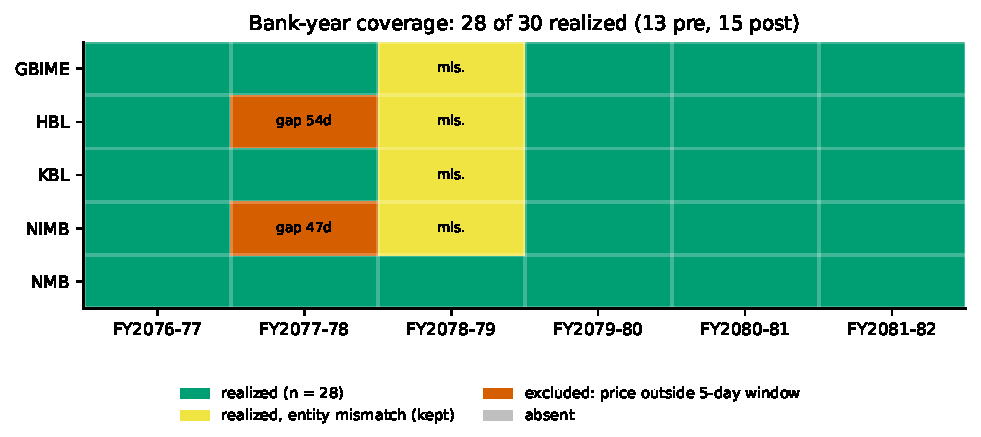
\includegraphics[width=0.90\textwidth]{figures/A1_coverage_map.pdf}
\caption{Panel Data Coverage Map across Bank Series and Fiscal Years}
\label{fig:app_coverage_map}
\end{figure}


\chapter{Complete Analysis Dataset}
\label{app:analysis_dataset}

This appendix presents the complete, verified empirical dataset compiled for the five sampled Nepalese commercial bank series across the six-year observation period (FY 2076/77 through FY 2081/82). 

Table~\ref{tab:app_dataset} presents all 30 planned bank-year observations, detailing secondary market prices observed immediately following statutory reporting deadlines ($MPS^{RD}$), reported basic earnings per share (EPS), recomputed book value per share (BVPS), cash dividend per share (DPS), and return on assets (ROA). Exactly 28 bank-years are realized in the analysis sample, with the two window-excluded observations clearly flagged.

\begin{table}[!htbp]
\centering
\small
\caption{Empirical Dataset: Accounting Fundamentals and Market Prices by Bank-Year}
\label{tab:app_dataset}
\begin{tabular}{lllccccc}
\toprule
\textbf{Bank} & \textbf{Fiscal Year} & \textbf{Regime} & \textbf{\shortstack{$MPS^{RD}$\\(NPR)}} & \textbf{\shortstack{EPS\\(NPR)}} & \textbf{\shortstack{BVPS\\(NPR)}} & \textbf{\shortstack{DPS\\(NPR)}} & \textbf{\shortstack{ROA\\(\%)}} \\
\midrule
GBIME & FY 2076/77 & Pre  & 450.00 & 17.99 & 151.95 & 2.00  & 1.37 \\
GBIME & FY 2077/78 & Pre  & 299.70 & 19.25 & 151.26 & 3.50  & 1.35 \\
GBIME & FY 2078/79 & Pre  & 189.00 & 20.84 & 158.60 & 10.60 & 1.40 \\
GBIME & FY 2079/80 & Post & 179.00 & 22.06 & 165.09 & 8.00  & 1.51 \\
GBIME & FY 2080/81 & Post & 218.69 & 16.99 & 169.97 & 0.00  & 1.08 \\
GBIME & FY 2081/82 & Post & 238.00 & 13.32 & 174.80 & 8.00  & 0.79 \\
\midrule
HBL   & FY 2076/77 & Pre  & 520.00 & 27.60 & 187.67 & 6.00  & 1.79 \\
HBL   & FY 2077/78 & Pre  & \textit{Excluded}$^a$ & 28.07 & 188.43 & 4.62  & 1.79 \\
HBL   & FY 2078/79 & Pre  & 231.00 & 18.26 & 169.72 & 11.11 & 1.20 \\
HBL   & FY 2079/80 & Post & 183.00 & 9.18  & 155.29 & 0.00  & 0.57 \\
HBL   & FY 2080/81 & Post & 231.07 & 5.72  & 169.11 & 0.00  & 0.36 \\
HBL   & FY 2081/82 & Post & 208.50 & 0.60  & 169.11 & 0.00  & 0.04 \\
\midrule
KBL   & FY 2076/77 & Pre  & 328.00 & 12.08 & 137.92 & 3.15  & 0.90 \\
KBL   & FY 2077/78 & Pre  & 222.00 & 14.20 & 136.13 & 2.67  & 1.17 \\
KBL   & FY 2078/79 & Pre  & 176.00 & 17.54 & 142.76 & 12.50 & 1.28 \\
KBL   & FY 2079/80 & Post & 136.90 & 1.97  & 134.66 & 0.00  & 0.17 \\
KBL   & FY 2080/81 & Post & 206.03 & 0.02  & 132.71 & 0.00  & 0.00 \\
KBL   & FY 2081/82 & Post & 229.00 & 6.94  & 141.53 & 0.00  & 0.43 \\
\midrule
NIMB  & FY 2076/77 & Pre  & 466.00 & 17.03 & 190.70 & 5.50  & 1.25 \\
NIMB  & FY 2077/78 & Pre  & \textit{Excluded}$^b$ & 22.00 & 198.28 & 3.39  & 1.65 \\
NIMB  & FY 2078/79 & Pre  & 191.00 & 20.74 & 185.67 & 7.00  & 1.61 \\
NIMB  & FY 2079/80 & Post & 156.00 & 13.92 & 162.92 & 0.00  & 1.08 \\
NIMB  & FY 2080/81 & Post & 211.51 & 12.04 & 176.31 & 0.00  & 0.88 \\
NIMB  & FY 2081/82 & Post & 210.70 & 12.69 & 190.40 & 0.00  & 0.82 \\
\midrule
NMB   & FY 2076/77 & Pre  & 437.00 & 12.62 & 150.06 & 3.20  & 1.09 \\
NMB   & FY 2077/78 & Pre  & 293.00 & 16.66 & 146.66 & 3.30  & 1.32 \\
NMB   & FY 2078/79 & Pre  & 235.00 & 17.92 & 146.30 & 8.25  & 1.35 \\
NMB   & FY 2079/80 & Post & 176.00 & 17.55 & 154.82 & 0.00  & 1.19 \\
NMB   & FY 2080/81 & Post & 251.13 & 12.22 & 157.74 & 0.00  & 0.77 \\
NMB   & FY 2081/82 & Post & 248.40 & 15.54 & 175.18 & 5.00  & 0.88 \\
\bottomrule
\end{tabular}

\vspace{4pt}
\begin{minipage}{\linewidth}
\footnotesize
\textit{Note.} $MPS^{RD}$ represents the NEPSE secondary market closing price on the first trading session following the statutory reporting deadline (end of Chaitra / mid-April; 5-day freshness window). BVPS is recomputed from published balance-sheet equity components; minor variances (0.28--0.40 NPR) with printed NAV in five NIMB rows reflect whole-integer rounding in printed highlights, while NMB FY 2081/82 (175.18 vs.\ 174.49) remains flagged as an unrounded reporting difference. Reported basic EPS uses weighted-average shares per NAS 33, while BVPS uses year-end shares; in merger year FY 2079/80, EPS denominators reflect blended share weights whereas BVPS uses post-merger ending shares. Variant R8 substitutes restated basic EPS for GBIME FY 2076/77 and NMB FY 2077/78. $^a$HBL FY 2077/78 price resumed 54 days late on 6 June 2022 (NPR 358.90). $^b$NIMB FY 2077/78 price resumed 47 days late on 30 May 2022 (NPR 367.70). Both excluded under the 5-day freshness rule.
\end{minipage}
\end{table}


\chapter{Model 2 Residual Diagnostics and Robustness Plots}
\label{app:diagnostics_robustness}

This appendix presents additional graphical diagnostic evaluations for Model~2 and the comparative robustness forest across the full eightfold sensitivity suite (R1 through R8).

Figure~\ref{fig:app_robustness_forest} presents the coefficient forest plot contrasting parameter estimates and 95\% HC3 confidence intervals across all eight robustness specifications.

\begin{figure}[!htbp]
\centering
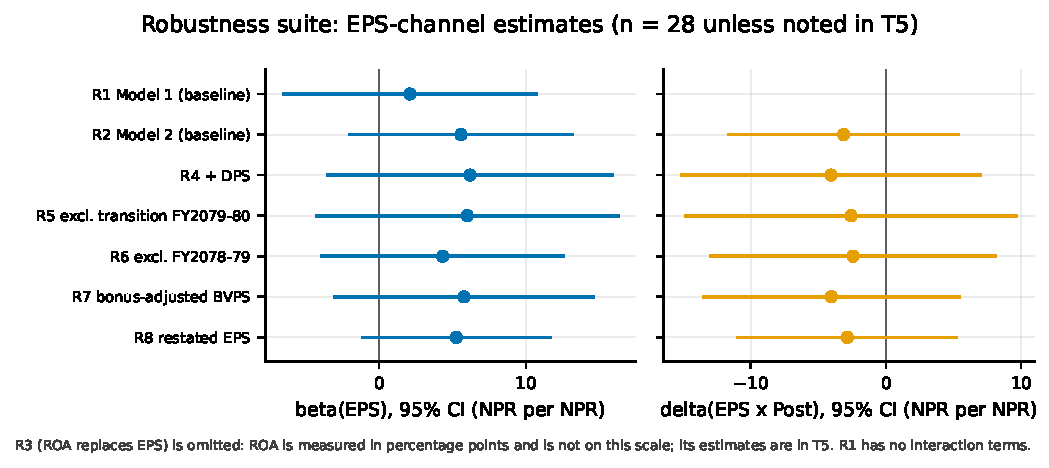
\includegraphics[width=0.88\textwidth]{figures/A2_robustness_forest.pdf}
\caption{Comparative Coefficient Forest Plot Across Robustness Specifications R1–R8}
\label{fig:app_robustness_forest}
\end{figure}

Figure~\ref{fig:app_model2_diagnostics} illustrates the four-panel econometric diagnostic suite evaluated on Model~2 residuals, examining linearity, residual normality, heteroskedasticity, and influential observations.

\begin{figure}[!htbp]
\centering
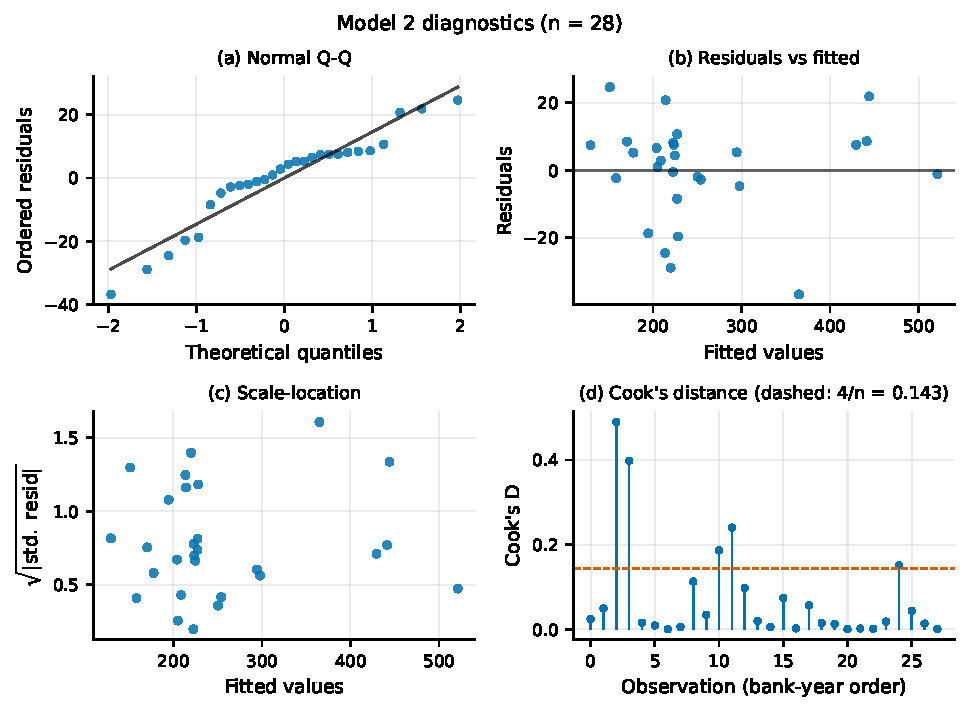
\includegraphics[width=0.88\textwidth]{figures/A3_model2_diagnostics.pdf}
\caption{Econometric Diagnostic Panel for Model 2 Residuals}
\label{fig:app_model2_diagnostics}
\end{figure}



\end{document}
